\documentclass[a4paper, 12pt]{report}
\usepackage[bottom,flushmargin,hang,multiple]{footmisc}
\listfiles
\usepackage[autostyle]{csquotes}
%% Title Definition Packages & Commands %%
\usepackage{titlesec}
\titleformat
{\chapter}
	[display]
	{\bfseries\LARGE}
	{Chapter \thechapter}
	{0pt}
	{
		\rule{\textwidth}{1pt}
		\centering
	}
	[
		\rule{\textwidth}{0.3pt}
	]
\titlespacing{\chapter}{0pt}{10pt}{10pt}

\renewcommand{\paragraph}[1]{\paragraph{#1}\mbox{}\\}
%%%%



\usepackage{enumitem}

\usepackage{fontawesome}

%% Geometry Packages & Commands %%
\usepackage[a4paper]{geometry}
\pdfoutput=1
%%%%

%% ICLR Conference Packages & Commands %%
%% \usepackage{preiclr,times}
\usepackage{iclr2017_conference,times}
\iclrfinalcopy
\setlength{\bibsep}{2pt}
%%%%

%% Bibliography Package %%
\usepackage[english]{babel}
\addto{\captionsenglish}{\renewcommand{\abstractname}{Executive Summary}}
%%%%

%% Packages from the American Mathematical Society %%
\usepackage{amssymb}
\usepackage{amsfonts}
\usepackage{amsmath}
\usepackage{physics}
%%%%

%% Graphics Packages & Commands %%
\usepackage{graphicx}
\graphicspath{{../graphics/}}
%%%%

%% Font Packages %%
\usepackage[default]{sourcesanspro}
\usepackage[T1]{fontenc}
%%%%

%% Color Package & Command %%
\usepackage{xcolor}
\definecolor{red-secondary-dark}{RGB}{205,32,38}
\definecolor{blue-primary-alt}{RGB}{2,191,231}
\definecolor{red-secondary}{RGB}{227,28,61}
%%%%

%% Reference Packages & Commands %%
\usepackage{url}
\usepackage{hyperref}
\usepackage{cleveref}
\usepackage{amsthm}
\newtheorem{conjecture}{Conjecture}
\newtheorem{theorem}{Theorem}
\newtheorem{lemma}{Lemma}
\crefname{lemma}{Lemma}{Lemmas}
%%%%

%% Space Packages & Commands %%
\usepackage{setspace}
\newcommand\tab[1][1cm]{\hspace*{#1}}
%%%%

%% Caption Packages & Commands %%
\usepackage[rightcaption]{sidecap}
\usepackage[font={color=red-secondary-dark,small},figurename=Fig.,labelfont={it}]{caption}
\captionsetup[algorithm]{labelsep=colon}
%%%%

%% Box Packages & Commands %%
\usepackage{lmodern}
\usepackage[most]{tcolorbox}
\usepackage{tabularx}
\usepackage{colortbl} 
\newcolumntype{Y}{>{\centering\arraybackslash}X}
\newtcolorbox[blend into=tables]{colortable}[2][]{
	colback=white,
	tabularx*={\renewcommand{\arraystretch}{1.0}}{Y|Y|Y|Y|Y|Y},title={#2},boxrule=0.8pt, center title
	}
\newtcolorbox[blend into=figures]{blockfigure}[2][]
	{
		colback=white,
		float=!htbp,
		boxsep=1pt,
		left=1pt,
		right=1pt,
		top=1pt,
		bottom=1pt,
		center title,
		%%lifted shadow={1mm}{-2mm}{3mm}{0.1mm}{black!50!white},
		title={#2},
		every float=\centering,
		#1
	}
\newtcolorbox[blend into=figures]{inlinefigure}[2][]
	{
		colback=white,
		boxsep=0.5pt,
		left=1pt,right=1pt,
		top=1pt,
		bottom=1pt,
		center title,
		%%lifted shadow={1mm}{-2mm}{3mm}{0.1mm}{black!50!white},
		title={#2},
		every float=\centering,
		#1
	}
%%%%

%% Code Packages %%
\usepackage{listings}
\usepackage{algorithm}
\usepackage{algorithmicx}
\usepackage{algpseudocode}
%%%%
\usepackage{textcomp}
		
\newtheorem{definition}{Definition}
\newtheorem{hypothesis}{Hypothesis}
\newtheorem{suggestedproof}{Suggested Proof}
\newtheorem{numericalanalysis}{Numerical Analysis}

\newcounter{examplecounter}
\newcommand{\example}[1]{\protect\stepcounter{examplecounter}\textbf{Example~\theexamplecounter:}~#1}

\newenvironment{nscenter}
{\parskip=0.2cm\par\nopagebreak\centering}
{\parskip=0pt\par\noindent\ignorespacesafterend}

\newenvironment{nsleft}
{\parskip=0pt\par\nopagebreak\raggedright}
{\parskip=0pt\par\noindent\ignorespacesafterend}



\begin{document}
\begin{titlepage}
	\begin{center}
		
\includegraphics[width=0.6\textwidth]{UnivAQ-logo}\\[1cm]
		{\LARGE University of L'Aquila}\\[0.5cm]
		{\large Department of Information Engineering, Computer Science and Mathematics}\\[0.5cm]
		\rule{\linewidth}{0.5mm} \\[0.4cm]
		{\huge \bfseries Hyper Heuristic Cryptography\\
			with\\
			Mixed Adversarial Nets \\[0.4cm] }
		\rule{\linewidth}{0.5mm} \\[0.1cm]
		\noindent
		{\large  \textsc{A Thesis conducted to acquire a Bachelor Degree In Computer Science}
			\vspace{-0.04cm} \\[0.01cm] }
		\rule{\linewidth}{0.5mm} \\[0.1cm]
		\noindent
			\begin{tcbraster}[raster columns=2,raster rows=1,
				enhanced,size=small,fit algorithm=hybrid* ]
					\begin{tcolorbox}[
						colback=white,
						sharp corners = northwest,
						title={Author}
						]
							\large
							\emph{Name :} \\[0.2cm]
							\tab Aly \textsc{Shmahell}\\[0.6cm]
							\emph{Signature :}\\[0.6cm]
							\rule{\linewidth}{0.5mm}
					\end{tcolorbox}
					\begin{tcolorbox}[
						colback=white,
						sharp corners = northwest,
						title = {Supervisor}
						]
							\large
							\emph{Name :} \\[0.2cm]
							\tab Prof.~Giovanni \textsc{De Gasperis}\\[0.6cm]
							\emph{Signature :}\\[0.6cm]
							\rule{\linewidth}{0.5mm}
					\end{tcolorbox}
			\end{tcbraster}
			\vspace{0.1cm}
		\today
	\end{center}
\end{titlepage}
\begin{titlepage}	
	\rule{\linewidth}{0.5mm} \\[0.1cm]
	\vspace{-0.1cm}
	\begin{minipage}{\textwidth}
		\Large{\textbf{Thesis Components}}
	\end{minipage}
	\rule{\linewidth}{0.2mm} \\[0.1cm]
	\noindent
		This thesis is comprised of the following parts:
		\begin{itemize}[nosep]
			\item A software project (codenamed "neurencoder") engineered to test the models presented in the thesis.
			\item This dissertation which serves as a documentation for the project, a presentation of its results, and a platform to explain the theories behind it.
		\end{itemize}	
		\vspace{-0.3cm}
	\rule{\linewidth}{0.2mm} \\[0.5cm]
	\noindent
	\rule{\linewidth}{0.5mm} \\[0.1cm]
	\begin{minipage}{0.5\textwidth}
		\Large{\textbf{Dissertation License}}
	\end{minipage}
	\begin{minipage}{0.5\textwidth}
		\begin{flushright}
			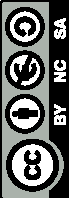
\includegraphics[angle=-90]{by-nc-sa}
		\end{flushright}
	\end{minipage}
	\\[0.1cm]
	\rule{\linewidth}{0.2mm}
	\vspace{-0.45cm}
	\begin{nscenter}
		This dissertation (in both source and compiled forms) is licensed under a\\
		\href{http://creativecommons.org/licenses/by-nc-sa/4.0/}{Creative Commons Attribution-NonCommercial-ShareAlike 4.0 International License.}
	\end{nscenter}	
	\rule{\linewidth}{0.2mm} \\[0.5cm]
	\noindent
	\rule{\linewidth}{0.5mm} \\[0.2cm]
	\begin{minipage}{0.5\textwidth}
		\Large{\textbf{Project License}}
	\end{minipage}
	\begin{minipage}{0.5\textwidth}
		\begin{flushright}
			\Huge{\textcopyright}
		\end{flushright}
	\end{minipage}
	\rule{\linewidth}{0.2mm}
	\noindent
	\vspace{-0.45cm}
	\begin{nscenter}
		The project presented in this dissertation, as well as its code (in both source and compiled forms) is copyrighted under the following terms:
	\end{nscenter}
	\vspace{-0.5cm}
	\begin{tcbraster}[raster columns=2,raster rows=1,
		enhanced,size=small,fit algorithm=hybrid* ]
		\begin{nscenter}
			\begin{tcolorbox}[colback=white]
				\begin{center}
					Copyright \textcopyright \space 2018, Aly Shmahell.\\
					All rights reserved.
				\end{center}
			\end{tcolorbox}
		\end{nscenter}
	\end{tcbraster}
	\rule{\linewidth}{0.2mm} \\[0.5cm]
	\noindent
	\rule{\linewidth}{0.5mm} \\[0.2cm]
	\begin{minipage}{\textwidth}
		\Large{\textbf{Project Repository \& Dissertation Publication}}
	\end{minipage}
	\rule{\linewidth}{0.2mm} \\[0.1cm]
	\noindent
	\vspace{-0.6cm}
		\begin{itemize}[nosep]
		\item A copy of this dissertation will be published on the author's Github account, on the day of discussion: 21-07-2018.
		\item The project's code resides on a private repository on the author's Gitlab account, to be available for review by academic researchers and industry professionals upon request.
		\end{itemize}	
		\vspace{-0.3cm}
	\rule{\linewidth}{0.5mm}\\[0.5cm]
	\noindent
		\rule{\linewidth}{0.5mm} \\[0.1cm]
		\begin{minipage}{0.5\textwidth}
			\Large{\textbf{Author's Contact Information}}
		\end{minipage}
		\vspace{-0.1cm}
		\\[0.1cm]
		\rule{\linewidth}{0.2mm} 
		\noindent
		\begin{nscenter}
			\begin{colortable}{}\faGithub & @AlyShmahell \\\hline
				\faGitlab & @AlyShmahell \\\hline
				\faTwitter & @AlyShmahell \\\hline
				\faLinkedinSquare &  www.linkedin.com/in/alyshmahell \\\hline
				\faInbox &  aly.shmahell@gmail.com \\\hline
			\end{colortable}
		\end{nscenter}
		\vspace{-0.5cm}
		\\[0.05cm]
		\rule{\linewidth}{0.2mm}
		\noindent
\end{titlepage}
\newpage
\chapter*{Abstract}
\begin{center}
	\begin{minipage}{0.8\textwidth}
			\justify
			It has been established that neural networks can learn to use encryption keys to protect information from other neural networks.
			The next question is, whether they can do it to a degree of efficacy that guarantees integrity of information alongside confidentiality.
			In this thesis, the goal is to enhance the heuristic methods employed in a neural-net-based multi-agent system to maximize confidentiality, while keeping loss of information-integrity to a minimum.
			We ask whether such a system, consisting of neural networks named Alice and Bob, can hold against an unknown malicious adversary which is a neural network named Alan, while having been training against a known helpful adversary which is a neural network named Eve, with the fact that both adversaries have access to the information channel between Alice and Bob, and thus acting as eavesdroppers.
			This thesis finally tries to put what the system has learned in one setting (asymmetric cryptography) to use in another (symmetric cryptography), by employing transfer learning.
			This thesis explores the theoretical basics behind neural cryptography, and provides software-engineered research-based empirical evidence for its results.
	\end{minipage}
\end{center}
\newpage
\begin{spacing}{0.05}
\tableofcontents
\end{spacing}
\newpage
\chapter{Introduction}\label{sec:introduction}
\begin{definition}
	(Neural Cryptography): is an interdisciplinary field in Computer Science, combining both artificial intelligence and cryptography, towards the development of stochastic methods, based on artificial neural networks, for use in encryption and cryptanalysis.
\end{definition}
\section{\textbf{Thesis Objectives}}
The objective of this thesis is to explore the use of new developments in the field of neural networks, mainly adversarial neural networks and convolutional neural networks, as a generative model, to produce a new breed of crypto-systems.\\\\
The work being done here is based on a new paper released in 2016 from Google Brain ~\citep{DBLP:journals/corr/AbadiA16}, which promises to bridge the gap between research and application in the area of neural cryptography.\\\\
The goal of my research is to provide the following:
\begin{itemize}
	\item An addition to the variety of the underlying neural-building methods provided in the original paper.
	\item An improvement in performance of the models being built.
	\item An in-depth analysis of how the components work, the mathematical \&  algorithmic mechanisms behind them.
	\item A software documentation that provides a blueprint for a more software-engineering oriented prototype of a neural crypto-system.
\end{itemize}
With the research specter in this area being dominated by authors coming from a mathematical-background, my thesis aims to provide:
\begin{itemize}
	\item A Computer Science oriented approach to solving cryptography with neural networks and stochastic methods, explained using vocabulary and notions geared towards Computer Scientists.
\end{itemize}
This thesis finally adds the following:
\begin{itemize}
	\item The introduction of a hybrid neural crypto-system that utilizes transfer-learning.\citep{5288526}
	\item An exploration into adding hyper heuristics to neural cryptography.
\end{itemize}
\newpage
\section{\textbf{Thesis Motivation}}
The question of motivation behind an idea can be empirically divided into:
\begin{itemize}[nosep]
	\item How would the author justify the importance of the idea?
	\item How would the author justify the viability of the idea?
\end{itemize}
\subsection{\textbf{Justification for the importance of Neural Cryptography}}
The age of intelligent machines is comprised of multiple intricate components, but individually they function narrowly even for the simplest of tasks. However, the surge of incorporation of these multiple components into one backbone that is neural-nets, has put artificial intelligence on a fast track towards competence in multiple complex areas of problem solving, surpassing traditional methods by multitudes on many occasions.\\
It makes sense from an academic perspective that we want neural nets to incorporate an understanding of cryptography, this would propel them closer to achieving general intelligence status, which is a major drive behind research in the field.\\
It also makes sense from an economic and existential point that we want neural nets to parallel their success in surpassing traditional methods when it comes to cryptography, because cryptography from a traditional sense is static, it always requires mathematicians and computer scientists to come together to patch it and upgrade it, and it is also always under attack, its mathematical models are always being broken and bent with the advancement in computer-power and the incorporation of new mathematical models into software that can break it.
Having neural nets as a dynamic generative model is an opportunity to gain an upper hand on bad actors and put cryptography in a more reactive state to protect our sensitive infrastructure, it would still require research and development, but it would put the neural net on the front line by dynamically devising new ways to mitigate risk and reformulate a cryptographic solution on the fly.
\subsection{\textbf{Justification for the viability of Neural Cryptography}}
This boils down to multiple general factors:
\begin{itemize}[nosep]
	\item \textbf{Neural Nets are viable general function approximaters:} The incorporation of multiple heuristic methodologies into neural nets has made them tackle a rapidly growing heap of complex tasks, cryptography is just another human invention to be caught up with.
	\item \textbf{Neural Nets are becoming faster:} The increasing successful research into using these heuristics not just to compute a complex task, but to do it quickly without loss in accuracy.
	\item \textbf{Neural Nets are becoming available:} The introduction of tools, frameworks and libraries of industrial level to the public which propelled the field of neural networks and made it ever so easy to replicate experiments and improve upon them.
\end{itemize}
Which lead to these thesis-related factors:
\begin{itemize}[nosep]
	\item \textbf{Neural Cryptography is viable:} The introduction of convolutional networks provides a well tested and understood methodology in reducing problems where local spatial relations in the data matter, which is the case for cryptography.\textsuperscript{\ref{footnote:1}}
	\item \textbf{Neural Cryptanalysis is viable:} Having a mixed convolutional net with fully connected layers will teach the network to account for global spatial relations as well, which teaches the net to learn and counter cryptanalysis.\textsuperscript{\ref{footnote:1}}
	\item \textbf{Neural Cryptography can be fast:} A result of using convolutions is that the small-sized pattern-finding filter has shared weights (and biases) for all spatial locations which the convolution processes, and this reduces the compute-power required for the whole process compared to other network models.
	\item \textbf{Neural Cryptography is evolved opposite to being patched:} Adversarial computation has been proven to be effective for years in the form of Genetic Algorithms, and adding adversary as a non-supervised generative model provides a better and easier experiment on how to synthesize a new form of cryptography.
\end{itemize}
\footnotetext[1]{Spatial Relations in Cryptography and Cryptanalysis can be found in the Appendix on page~\pageref{appendix:1}.\label{footnote:1}}
\newpage
\section{\textbf{Previous Work}}
The work being done so far in neural cryptography can be divided to old (pre 2016), and new (post 2016). For the old section, this thesis will only list the works and attributions without delving into the details.
\subsection{\textbf{Previous Work - Pre 2016 Era}}
Up until 2010, Neural Nets were a dark alley in the citadel of artificial intelligence, mainly due to lack in advancement in back-propagation optimization which made training deep neural nets hard, and the fact that not many people saw the importance of incorporating other areas of artificial intelligence into neural nets.\\
From 2010 until 2016, things started changing for the better, but it was 6 years until the developments allowed for new viable research in neural cryptography.\\
Therefor the works in the Pre 2016 Era were merely academic curiosities which did not aim to make it into industry, but they provided a key stepping stone for those of us who came into the field at this better-equipped stage.\\\\
The most notable of these works are:
\begin{itemize}[nosep]
	\item The first definition of the Neuro-Cryptography (AI Neural-Cryptography) applied to DES cryptanalysis. ~\citep{s.dourlens.free.fr/AppliedNeuroCryptography}
	\item Permutation parity machines for neural synchronization ~\citep{1751-8121-42-19-195002}
	\item Permutation parity machines for neural cryptography ~\citep{PhysRevE.81.066117}
	\item Successful attack on permutation-parity-machine-based neural cryptography ~\citep{PhysRevE.85.025101}
\end{itemize}
\subsection{\textbf{Previous Work - Post 2016 Era}}
In the period 2010 - 2016, a surge of new ideas came into play in the field of neural nets, new methods of back-propagation optimization proved to be successful for deep-learning, advancement in initialization and activation solved multitudes of problems like the vanishing gradient (or at least mitigated its effect), ...etc, so it was only natural someone would attempt to take another look at neural cryptography, and the most notable works so far are:
\begin{itemize}[nosep]
	\item \textbf{Learning to Protect Communications with Adversarial Neural Cryptography} ~\citep{DBLP:journals/corr/AbadiA16}:\\
	This paper was the corner stone for my work, it was the first to realize the importance of using generative adversarial nets in cryptography and succeed in its efforts to build a viable neural crypto-system.
	\item \textbf{Tensorflow implementation of Adversarial Neural Cryptography} ~\citep{ankeshanand/neural-cryptography-tensorflow}:\\
	Ankesh Anand's Implementation of (Learning to Protect Communications with Adversarial Neural Cryptography) using Tensorflow and Python is a very informative open-source prototype which I studied before I set on implementing my project.
	\item \textbf{Adversarial Neural Cryptography in Theano} ~\citep{nlml/adversarial-neural-cryptography}:\\
	Liam Schoneveld made an implementation of (Learning to Protect Communications with Adversarial Neural Cryptography) in Theano and Python, his results mirror mine to some extent, and his illustrations and break-down of the process is something to consider going over when delving into neural cryptography.
\end{itemize}
\newpage
\chapter{Design}\label{sec:design}
This chapter deals with the inner-mechanics of how convolutional neural nets work, which are the building blocks for the adversarial crypto-system built for this thesis.\\
This chapter serves to provide a theoretical basis for much of the basics and the enhancements researched for the thesis.\\
As a way to illustrate how a convolutional neural network (ConvNet) should be constructed for the purposes of this thesis, a simplified dummy example is presented and dissected to explain how its components work.\\
\begin{blockfigure}{Graph Diagram for an Example Dummy ConvNet}\label{fig:SimpleNetDiagram}
	\begin{center}
		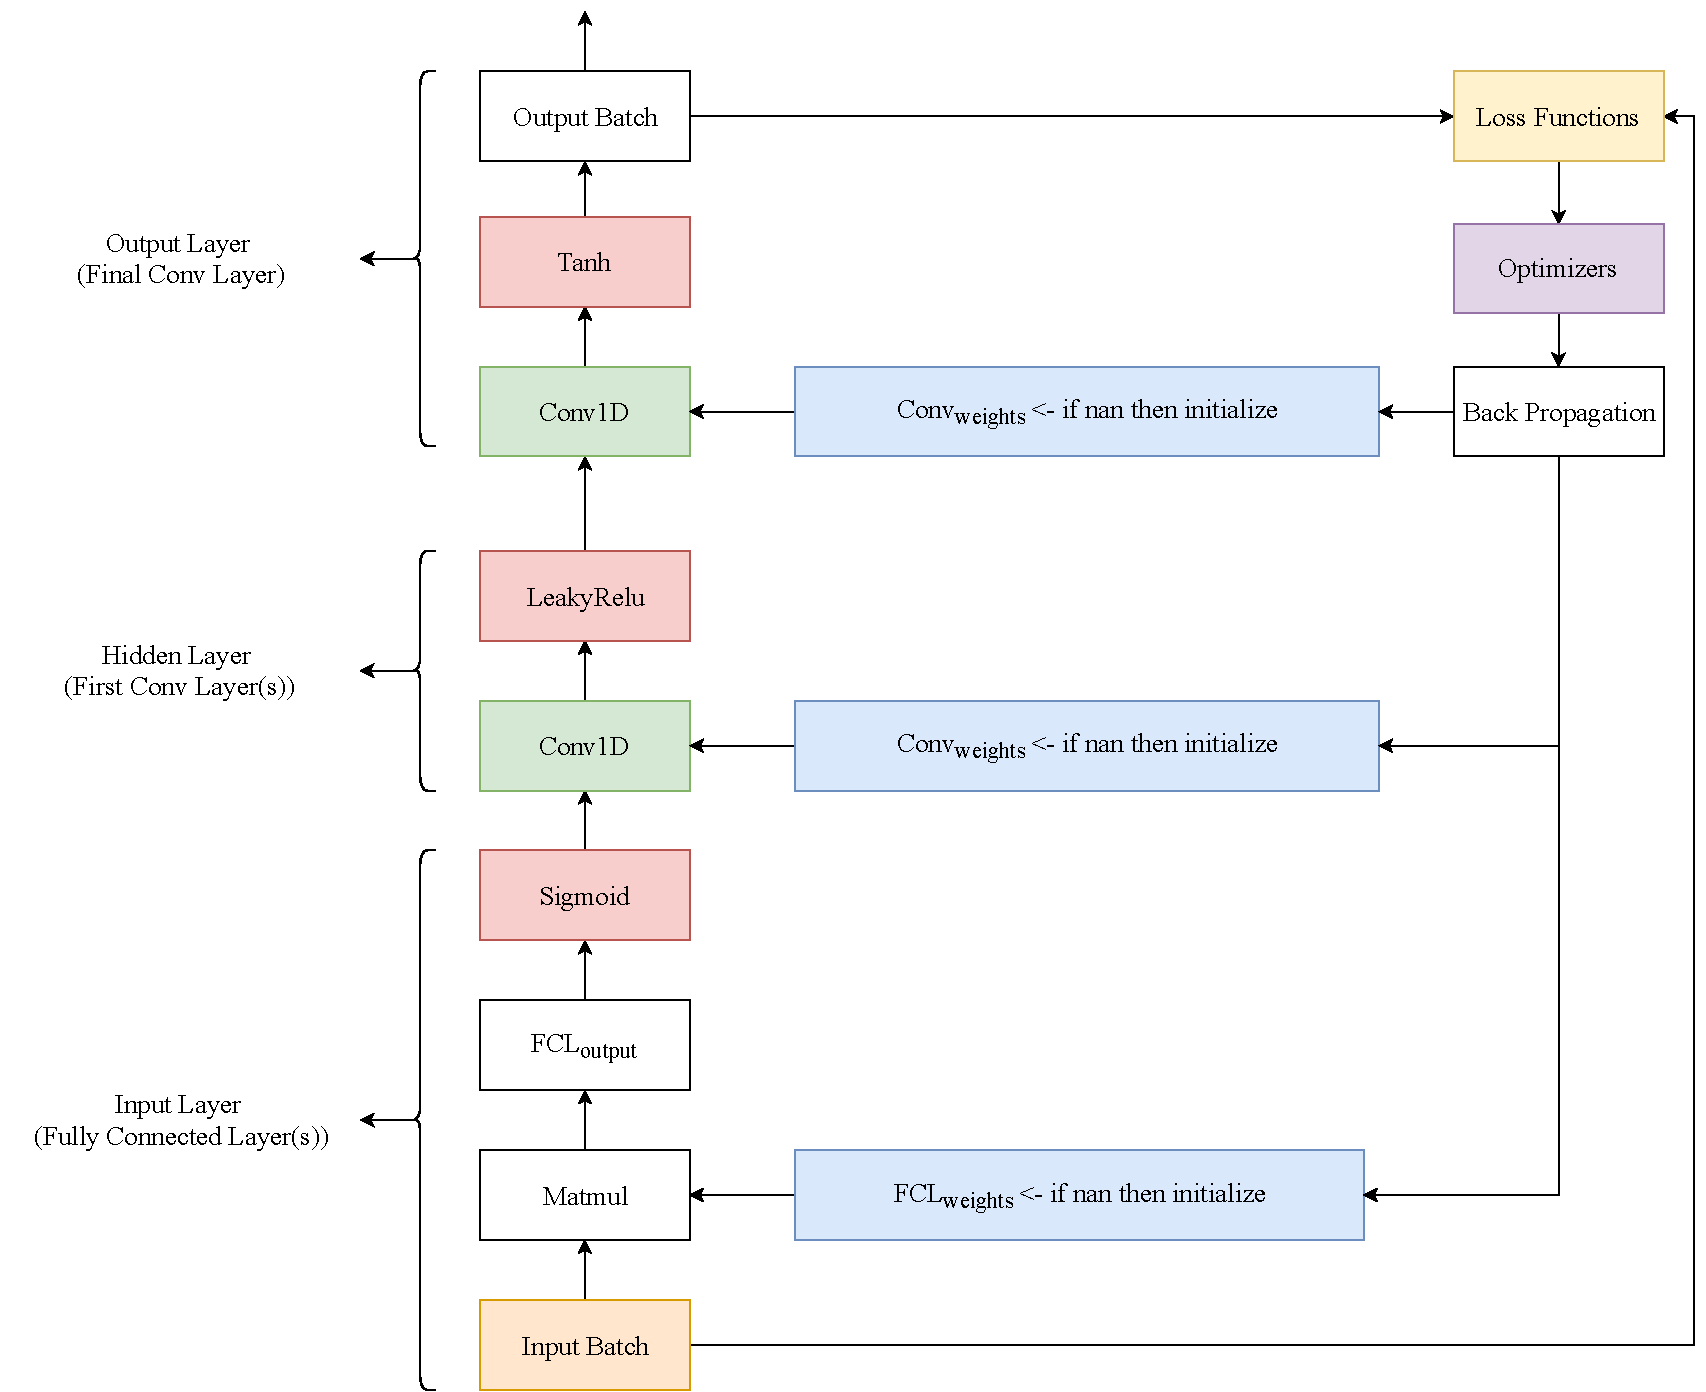
\includegraphics[height = 0.45\textheight]{SimpleNetDiagram}
	\end{center}
\end{blockfigure}\\
This ConvNet has 6 key components which we will go over as the following:
\begin{itemize}[nosep]
	\item Weight Initialization
	\item 1D Convolution
	\item Batches
	\item Activation Functions
	\item Loss Functions
	\item Optimization
\end{itemize}
\newpage
\section{\textbf{Weight Initialization}}
\begin{definition}
	(Weight Initialization): is the process in which we give some weight values to some neurons in some layer, the overall process, whether done properly or not means the difference between the network converging on a local/global minima versus never converging at all.
\end{definition}
\subsection{\textbf{Xavier Initialization} ~\citep{DBLP:journals/jmlr/GlorotB10}  }
\begin{lemma}\label{lemma1}
Suppose our net uses the hyperbolic tangent activation function for its neurons:\\
\begin{blockfigure}{Example Plot of the Hyperbolic Tangent}
	\[ 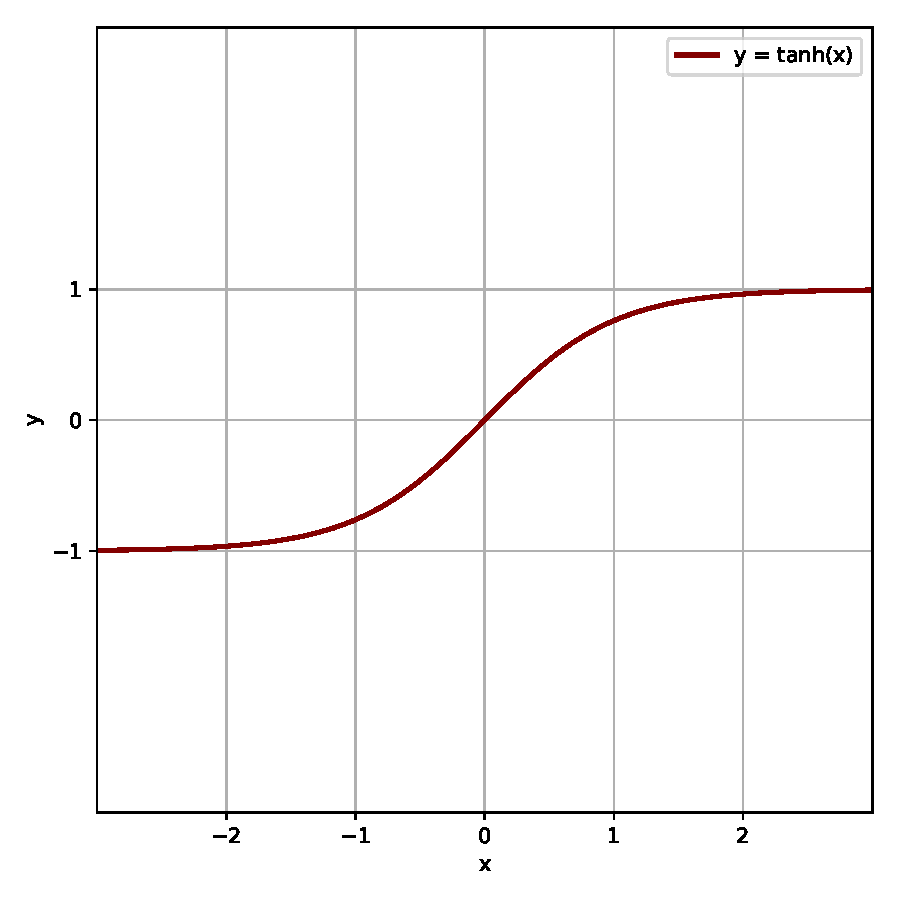
\includegraphics[width=0.7\textwidth]{tanh} \]
\end{blockfigure}
\begin{itemize}
	\item If the weights start too small, then the signal shrinks as it passes through each layer until it vanishes ~\citep{an-explanation-of-xavier-initialization}, then as it passes deeper in the network with its small values, the layers it enter will become linear, because the output of the hyperbolic tangent is linear with small input values, this means the deeper layers of the net will loose non-linearity.
	\item If the weights start too large, then the signal grows as it passes through each layer until it becomes too large ~\citep{an-explanation-of-xavier-initialization}, then as it passes deeper in the network with its large values, the layers it enter will become saturated, as the output of the hyperbolic tangent is large \& flat with large input values, and this flatness will cause the gradient to become zero, and we will get the vanishing gradient problem.
\end{itemize}
\end{lemma}
\begin{lemma}\label{lemma2}
Having a pre-defined net graph: for each neuron "$ n $" we know the number of inputs and the number of outputs, therefor we can calculate a reasonable weight for the neuron in question based on a normal distribution of a zero mean and a 1/n variance.
\end{lemma}
\begin{lemma}\label{lemma3}
To achieve initialization while avoiding the two obstacles in \cref{lemma1}, we want the variance to remain the same with each passing layer.	
\end{lemma}
\newpage
Suppose we have an input X from a previous layer with $ n_{in} $ components and a linear neuron $ n $ with random weights W in the current layer that spits out the same output Y to some neurons in the next layer.
\begin{blockfigure}{Xavier Initialization on neuron "n"}
		\[ 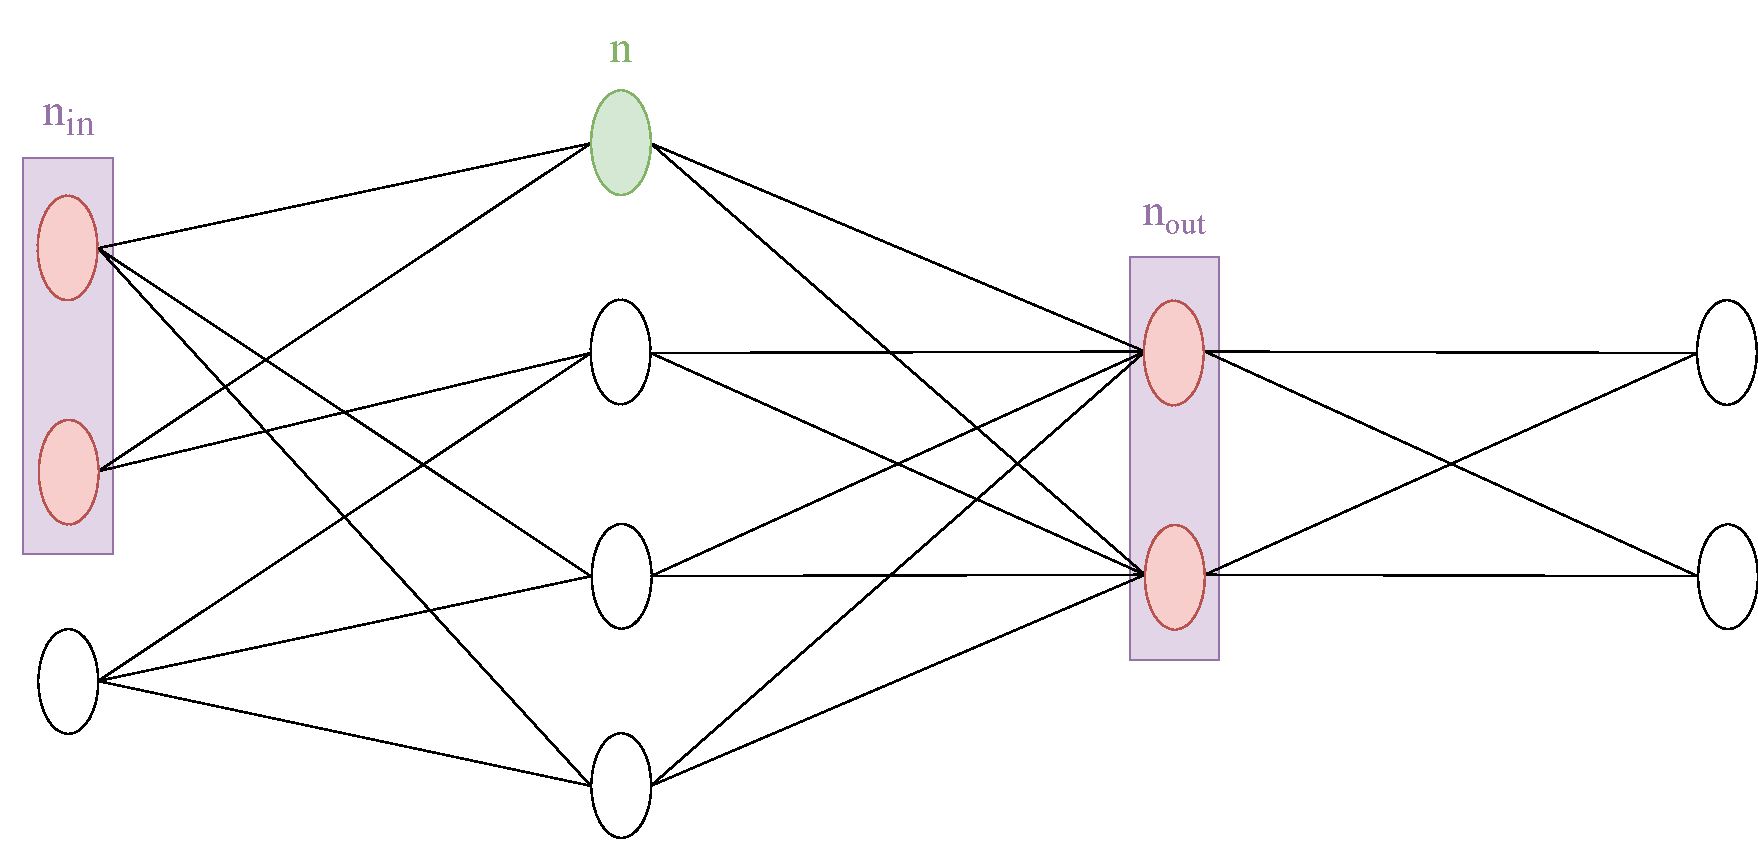
\includegraphics[width=0.6\textwidth]{xavier_illustration} \]
\end{blockfigure}\\
The output of the neuron will have the following equation:
\begin{center}
	\begin{equation}
		Y = W_1X_1 + W_2X_2 + ... + W_n X_n \label{eq:1}
	\end{equation}
\end{center}
To calculate the variance of each component:
\begin{center}
	\begin{equation}
		Var(W_iX_i) = E[X_i]^2 Var(W_i) + E[W_i]^2 Var(X_i) + Var(W_i)Var(X_i) \label{eq:2}
	\end{equation}
\end{center}
Since our inputs and weights come from a normal distribution of zero mean (from \cref{lemma2}):
\begin{center}
	\begin{equation}
		E[X_i]^2 Var(W_i) + E[W_i]^2 Var(X_i) = 0 \implies
		Var(W_iX_i) = Var(W_i)Var(X_i) \label{eq:3}
	\end{equation}
\end{center}
Since the neurons in the same previous layer are all independent, we assume that both $ X_i $ and $ W_i $  are independent and also identically distributed:
\begin{center}
	\begin{equation}
	 Var(Y) = Var(W_1X_1 + W_2X_2 + ... + W_n X_n) = nVar(W_i)Var(X_i) \label{eq:4}
	\end{equation}
\end{center}
In the last equation, we have the variance of the inputs, the variance of the output and the variance of the weights, now we can calculate the variance of the weights from ~\cref{lemma3}:
\begin{center}
	\begin{equation}
	 Var(Y) = Var(X_i) \implies Var(W_i) = \frac{1}{n_{in}} \implies Var(W_i) * n_{in} = 1  \label{eq:5}
	\end{equation}
\end{center}
Now if we go through the same derivation for back-propagation, we get:
\begin{center}
	\begin{equation}
	Var(W_i) = \frac{1}{n_{out}} \implies Var(W_i) * n_{out} = 1 \label{eq:6}
	\end{equation}
\end{center}
To keep the variance of the input gradient \& the output gradient the same, we combine
\eqref{eq:5} \& \eqref{eq:6} and we get:
\begin{center}
	\begin{equation}
	(n_{out} + n_{in}) * Var(W_i) = 2 \implies Var(W_i) = \frac{2}{n_{in} + n_{out}} \label{eq:7}
	\end{equation}
\end{center}
\newpage
\section{\textbf{1D Convolution}}\label{Conv1D}
\begin{definition}
	(1D Convolution): is the process of using a small window to determine local spatial relations over a 1D data sample, regardless of whether the sample is inside an n-D data batch.
\end{definition}
When looking for examples and literature on convolution, the vast majority of what is available is on 2D Convolution, and what might be found on 1D Convolution is usually done on 1D data with 1D filters~\citep{math-behind-1d-convolution-with-advanced-examples-in-tf}.
Therefor, for the purposes of this study, a more complex example of 1D Convolution will be presented.\\\\

\textbf{Note:} This section on 1D Convolution with its explanations, Pseudo-Code and examples, was reconstructed from practical experiments designed to understand 1D Convolution, implemented by the author in Tensorflow and Python.\\
The source code for the Tensorflow 1D Convolution operation (conv1d) was studied briefly, and it seems it is implemented by forcing 1D Convolution (conv2d) to perform convolution over just one axis in the batch, but in this thesis the focus will be on reconstructing 1D Convolution on its own.\\
\section{\textbf{1D Convolution on Batch 1D Data with (1,2)-D Filters}}
At this moment, the best tool available for representing data samples is \textbf{tensors}, and therefor determining local spatial relations amounts to matrix multiplications of the spatial locations inside the data sample tensor by the portion of the filter tensor that fits the location.\\
In order for the convolution to do these multiplications, it \textbf{slides} over one axis of the 1D data sample, the y-axis, the filter also \textbf{slides} itself to fit the location.\\
In order to perform 1D Convolution with a 2D filter (having an x-axis and a y-axis), we need to add another axis to both the data and the filter; done by injecting a z-axis into the y-axis, effectively expanding the y-axis over the z-axis. In this case, when the filter \textit{slides}~itself, it \textit{slides}~over its x-axis.\\
In this format, the window processing is done by multiplying the z-axis of the sample by the y-axis of the filter, over the x-axis of the filter.\\
Every \textit{slide} is done over a fixed length called a stride, and every \textit{slide} represents moving the filter window over to a new spatial location in the sample.\\
It is also important to note that since the stride determines how many steps to slide upon each time, it is synonymous to dividing the length of the z-axis of the final input over the stride length.\\
If instead of having one data sample, we have a batch of data samples, we perform convolution on the samples independently. This means the data batch has an extra axis, an x-axis.\\
This way, each time a convolution over a sample is done, the filter resets its \textbf{slided} position to its default, and the convolution \textbf{steps} onto the next sample over the x-axis of the batch.\\
Finally, we end up with a 3D tensor for the data batch, and another 3D tensor for the filter.\\
After the filter is done processing all the samples in the batch, the result tensor will be a 3D tensor with the following dimension lengths:
\begin{itemize}[nosep]
	\item $ result.xAxis.length = batch.xAxis.length $
	\item $ result.yAxis.length = filter.xAxis.length $
	\item $ result.zAxis.length = filter.zAxis.length $
\end{itemize}
Each entry over the x-axis of the result represent a processed sample, and if the z-axis of the result has $ length > 1 $, then each entry over the y-axis represents a feature map of the sample, each feature map has different derived information from the spatial location that was processed.\\
To illustrate how this works, I've chosen a flat representation of the 3D tensors (representing 3D with 2D), mainly because this is how it's done with Numpy, and this is more practical for Computer Scientists.
\begin{blockfigure}{Flat 2D Representation of 3D Tensors - Numpy Style}
		\begin{center}
			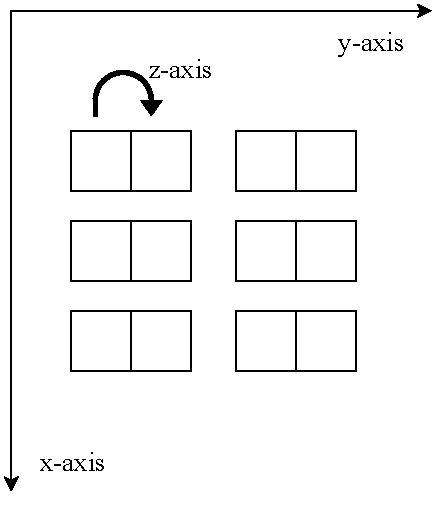
\includegraphics[height=0.21\textheight]{numpy-3Dtensor-axis}
		\end{center}
\end{blockfigure}
\newpage
\subsection{\textbf{1D Convolution Algorithm}}
\begin{lemma}\label{lemma4}
	The relation between the dimension lengths of the batch and the filter can be described as the following:
	\begin{itemize}[nosep]
		\item $ filter.xAxis.length >= 1 $
		\item $ filter.yAxis.length = batch.zAxis.length $
		\item $ filter.zAxis.length >= 1 $
	\end{itemize}
\end{lemma}
\begin{lemma}\label{lemma5}
	if $ filter.xAxis.length > batch.yAxis.length $, the filter is offset by an amount of $ filter\_offset =  filter\_x\_axis\_length - batch\_y\_axis\_length $ throughout the convolution process.
\end{lemma}
\begin{algorithm}
	\caption[]{1D Convolution Pseudo-Code}
	\begin{algorithmic}
		\State $ step = 0 $
		\If{$ filter.xAxis.length >  batch.yAxis.length$}
			\State $ filter.offset =  filter.xAxis.length - batch.yAxis.length $
		\Else
			\State $ filter.offset =  0 $
		\EndIf
		\While {$ step < batch.xAxis.length $}
			\State $ slide = 0 $
				\While {$ slide < batch.yAxis.length $}
					\State $ y = slide $
					\While {$ y <  batch.yAxis.length $}
						\State $ z = 0 $
						\While {$ z < filter.zAxis.length $}
							\begin{align*}
							\tab result[step][y][z]=
							\sum_{x=0}^{x<=filter.xAaxis.length}\biggl\{
							batch[step][x+slide][y] *\\ filter[x-slide+filter.offset][y][z]
							\biggr\} 
							\end{align*}
							\State $ z = z + 1 $
						\EndWhile
						\State $ y = y + 1 $
					\EndWhile
					\State $ slide = slide + 1 $
				\EndWhile
			\State $ step = step + 1 $
		\EndWhile
	\end{algorithmic}
\end{algorithm}
\newpage
\subsection{\textbf{Simple ConvNet Example with 2 Conv Layers}}
This example illustrates how stacked convolutions work, by feeding one Conv Layer output to the next one.\\\\
It also illustrates how 1D Convolution works on batch 1D data with 2D (expanded to 3D) filters in each Conv Layer.\\\\
For the sake of simplicity, in this example:
\begin{itemize}
	\item We will forsake the use of activation functions between layers.
	\item We will also use weights that are initialized manually and chosen arbitrarily.
	\item We will use a stride length of 1.
\end{itemize}
\begin{blockfigure}{Simple ConvNet with 2 Conv Layers}
	\begin{center}
		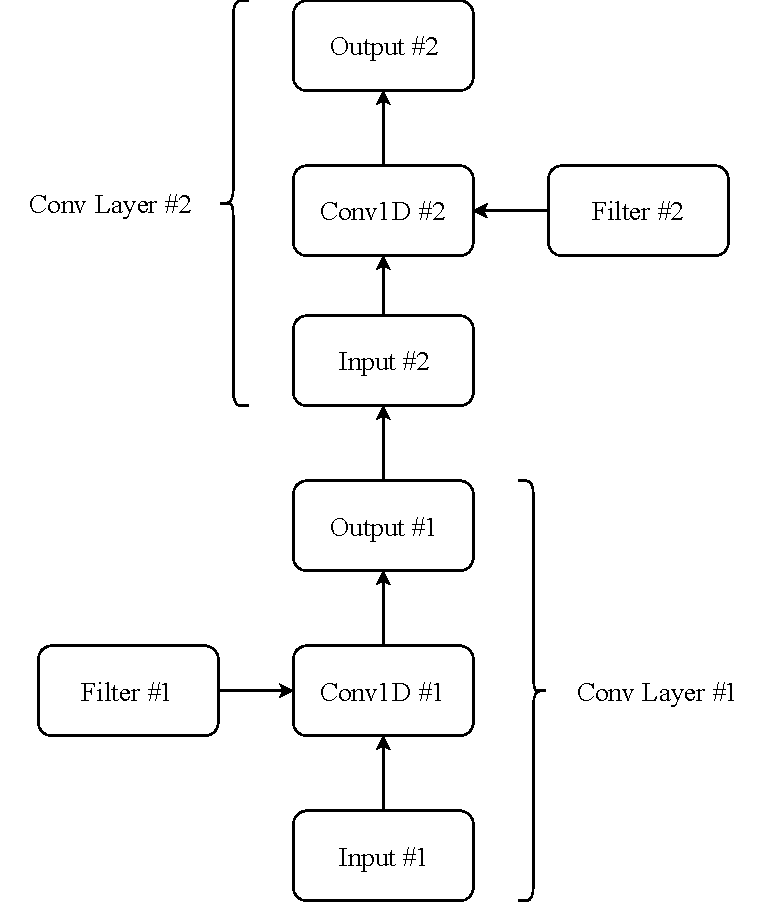
\includegraphics[width=0.9\textwidth]{convLayerExample}
	\end{center}
\end{blockfigure}
\newpage
	{
		
		\color{blue-primary-alt} 
		\rule{2.1cm}{0.4mm}\\[0.2cm]
		\textbf{Conv Layer \#1}\\
		\rule{2.1cm}{0.4mm}
	}\\\\
\tab The example starts off by generating 1D input strings.\\
\begin{tcbraster}[raster columns=3,raster rows=1,
	enhanced,size=small,fit algorithm=hybrid* ]
	\begin{inlinefigure}{First Input String}
		\begin{center}
			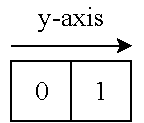
\includegraphics[width=0.5\textwidth]{input1}
		\end{center}
	\end{inlinefigure}
	\begin{inlinefigure}{Second Input String}
		\begin{center}
			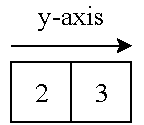
\includegraphics[width=0.5\textwidth]{input2}
		\end{center}
	\end{inlinefigure}
	\begin{inlinefigure}{Third Input String}
		\begin{center}
			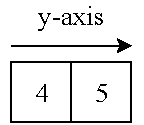
\includegraphics[width=0.5\textwidth]{input3}
		\end{center}
	\end{inlinefigure}
\end{tcbraster}
\begin{tcbraster}[raster columns=2,raster rows=1,
	enhanced,size=small,fit algorithm=hybrid* ]
	\begin{tcolorbox}[frame hidden,colback=white]
		\tab Input strings are then stacked up \tab along the x-axis to form a 2D batch.
	\end{tcolorbox}
	\begin{inlinefigure}{Input Batch}
		\begin{center}
			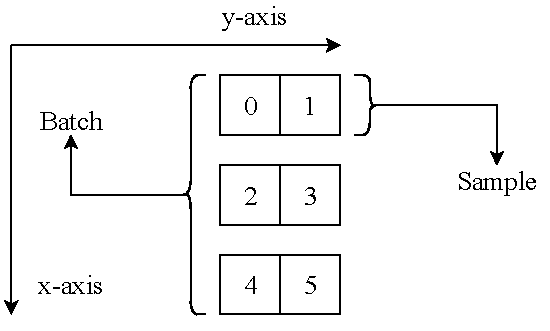
\includegraphics[width=\textwidth]{input_final}
		\end{center}
	\end{inlinefigure}
\end{tcbraster}

\begin{tcbraster}[raster columns=2,raster rows=1,
	enhanced,size=small,fit algorithm=hybrid* ]
	\begin{tcolorbox}[frame hidden,colback=white]
		\tab Then the batch gets expanded from \tab 2D to 3D along the y-axis (injecting z-\tab axis into y-axis), which means the\\\tab final batch shape becomes (3, 2, 1).
	\end{tcolorbox}
	\begin{inlinefigure}{Reshaped Input Batch}
		\begin{center}
			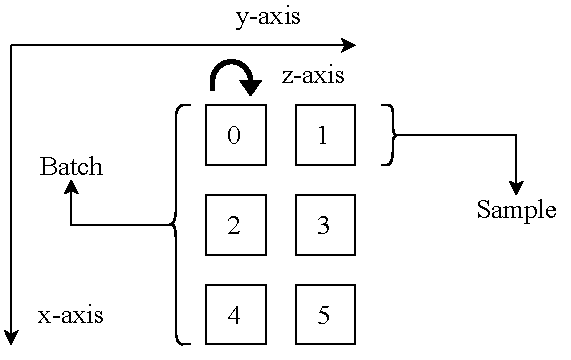
\includegraphics[width=\textwidth]{input_reshaped}
		\end{center}
	\end{inlinefigure}
\end{tcbraster}
\begin{tcbraster}[raster columns=2,raster rows=1,
	enhanced,size=small,fit algorithm=hybrid* ]
	\begin{tcolorbox}[frame hidden,colback=white]
		\tab Then finally, a filter of shape (2, 1, 2) is \tab provided for the convolution.
	\end{tcolorbox}
	\begin{inlinefigure}{Filter \#1 with Arbitrary Weights}
		\begin{center}
			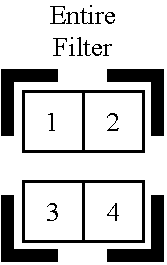
\includegraphics[width=0.34\textwidth]{filter1}
		\end{center}
	\end{inlinefigure}
\end{tcbraster}
\newpage
After the input batch tensor and the filter tensor have been generated, the convolution process can begin.\\
\begin{blockfigure}{ Applying the filter to the first sample in the input batch - generating the first value in the first feature map.}
	\begin{center}
		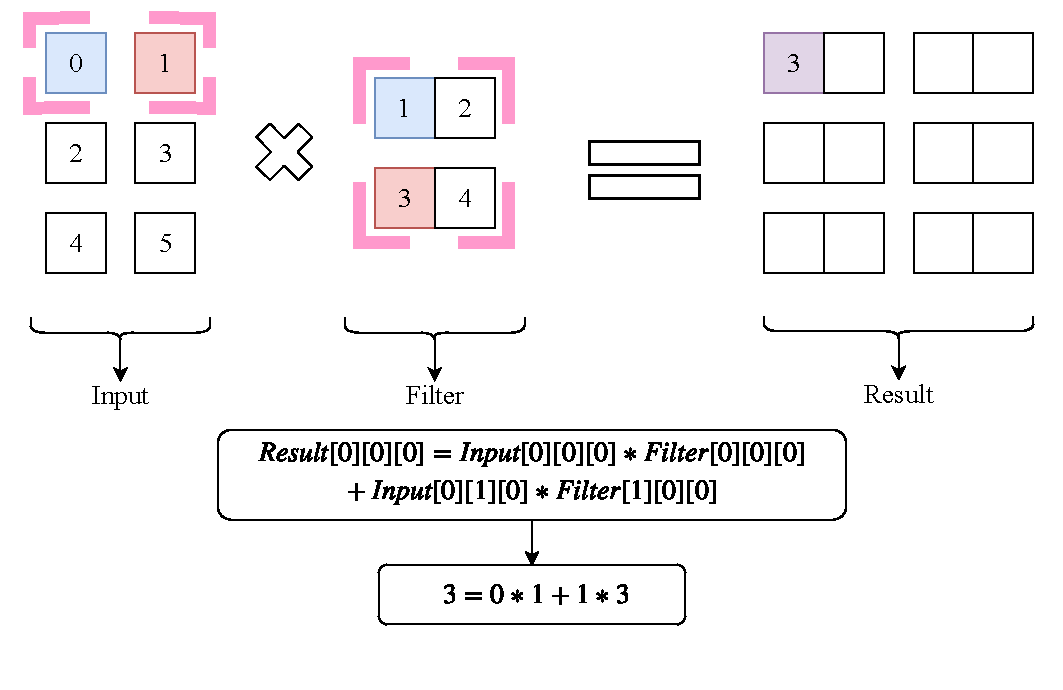
\includegraphics[width=\textwidth]{firstConvSample_step1}
	\end{center}
\end{blockfigure}
\begin{blockfigure}{ Applying the filter to the first sample in the input batch - generating the second value in the first feature map.}
	\begin{center}
		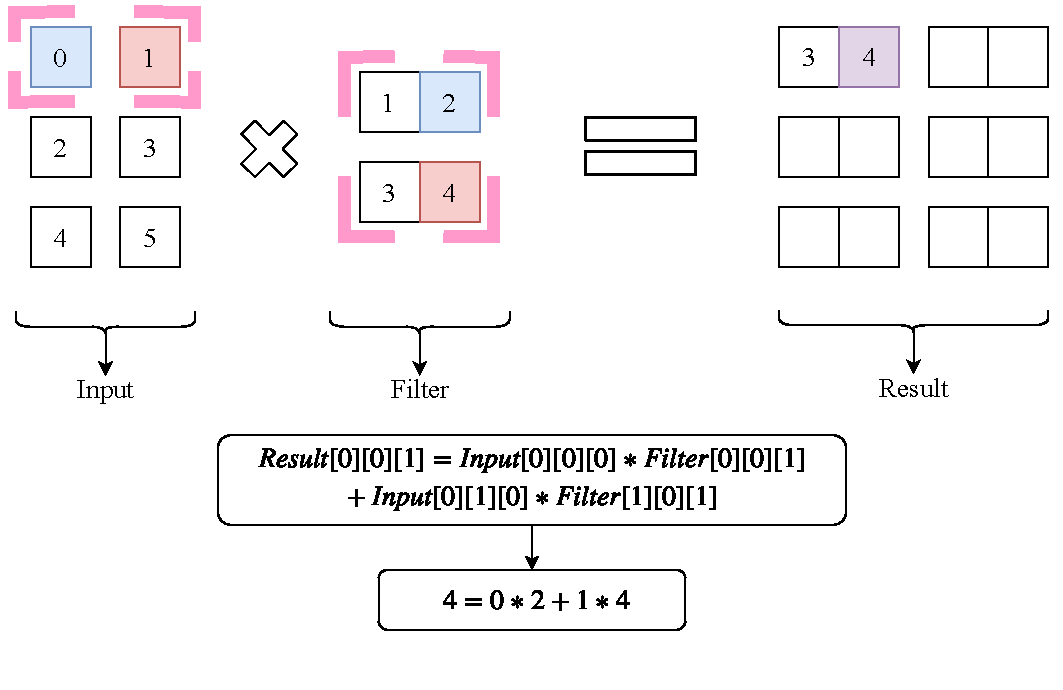
\includegraphics[width=\textwidth]{firstConvSample_step2}
	\end{center}
\end{blockfigure}
\newpage
\begin{blockfigure}{ Applying the filter to the first sample in the input batch - generating the second feature map.}
	\begin{center}
		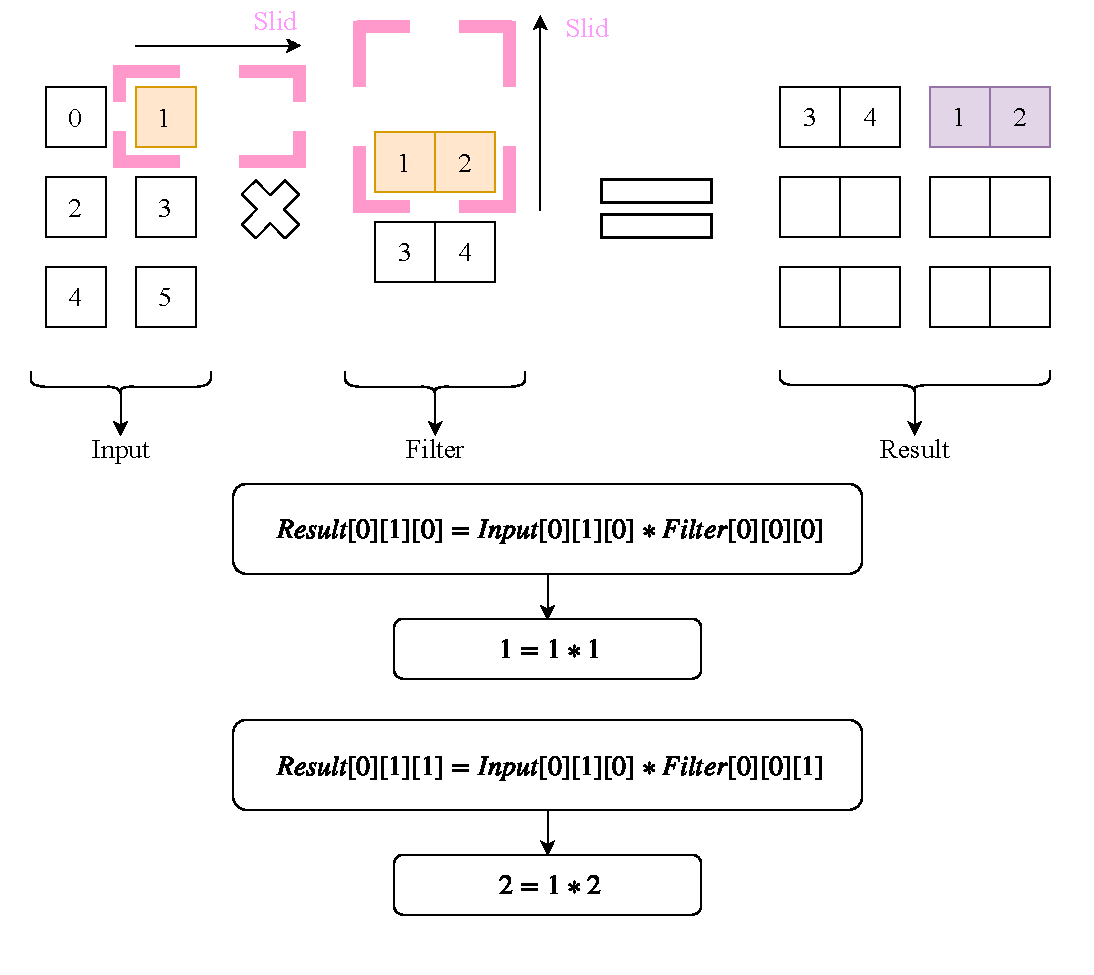
\includegraphics[width=\textwidth]{firstConvSample_step3}
	\end{center}
\end{blockfigure}
\begin{blockfigure}{ The entire convolution performed on the data batch.}
		\begin{center}
			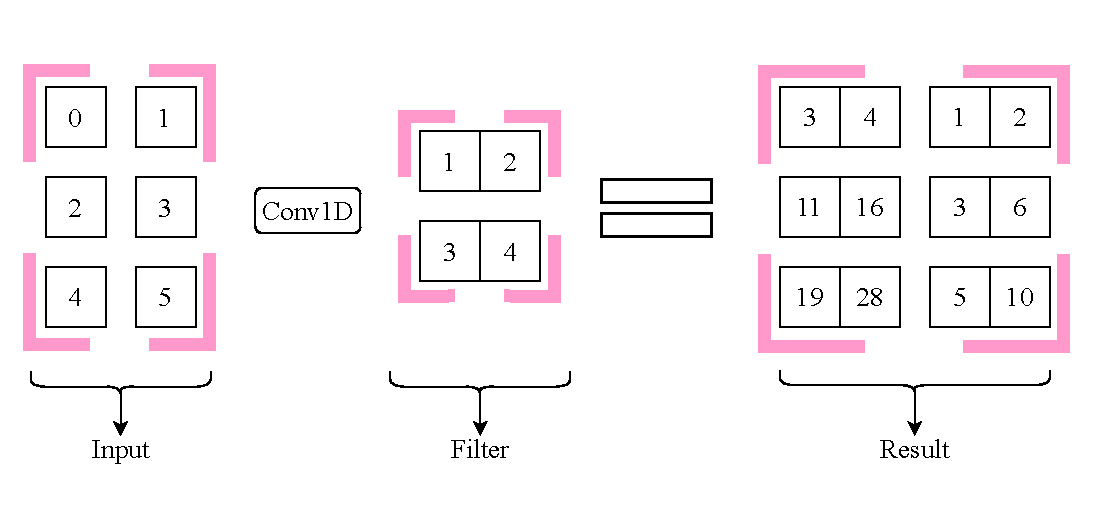
\includegraphics[width=\textwidth]{firstConvSample_final}
		\end{center}
\end{blockfigure}
\tab The resulting 3D tensor is of shape (3, 2, 2), and it contains 2 feature maps.
\newpage
	{
		
		\color{blue-primary-alt} 
		\rule{2.1cm}{0.4mm}\\[0.2cm]
		\textbf{Conv Layer \#2}\\
		\rule{2.1cm}{0.4mm}
	}\\\\
To continue with the example, the resulting tensor from \textbf{Conv Layer \#1} will be fed as input to \textbf{Conv Layer \#2}, for this purpose we need a new filter that conforms to the rules of matrix multiplication (taking into account the sliding rule), that is its y-axis has the same length as the z-axis from the tensor we're convolving on.\\\\
And for the sake of making the example closer to real-life usage, we will make the resulting tensor from \textit{Conv Layer \#2} have the same shape as the original input tensor by making the z-axis of the new filter of length 1, which will reduce the number of feature maps from 2 to 1, then by performing dimensionality reduction (squeezing of the z-axis onto the y-axis).\\\\
The shape of the newly constructed filter would be: (var, 2, 1), where $ var >= 1 $, in our example var = 3.
\begin{blockfigure}{The output from the first Conv Layer becomes input to the second Conv Layer}
	\begin{center}
		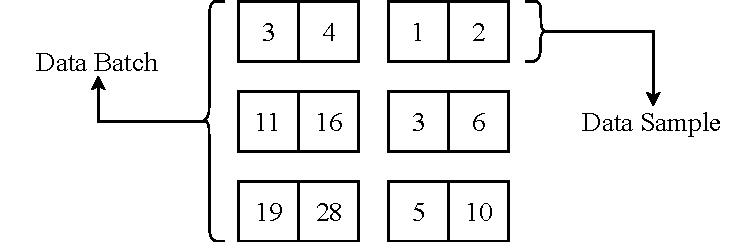
\includegraphics[width=\textwidth]{secondinput_final}
	\end{center}
\end{blockfigure}
\begin{tcbraster}[raster columns=2,raster rows=1,
	enhanced,size=small,fit algorithm=hybrid* ]
	\begin{tcolorbox}[frame hidden,colback=white]
		\tab A filter of shape (3, 2, 1) is provided \tab for the convolution.
	\end{tcolorbox}
	\begin{inlinefigure}{Filter \#2 with Arbitrary Weights}
		\begin{center}
			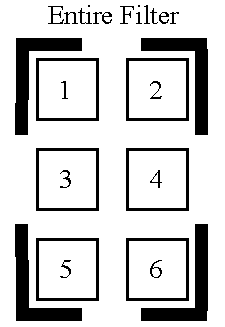
\includegraphics[height=0.25\textheight]{filter2}
		\end{center}
	\end{inlinefigure}
\end{tcbraster}
\newpage
After the input batch tensor has been provided the filter tensor has been generated, the convolution process can begin.\\
\begin{blockfigure}{ Extracting the first value from the first sample in the data tensor to the feature map.}
	\begin{center}
		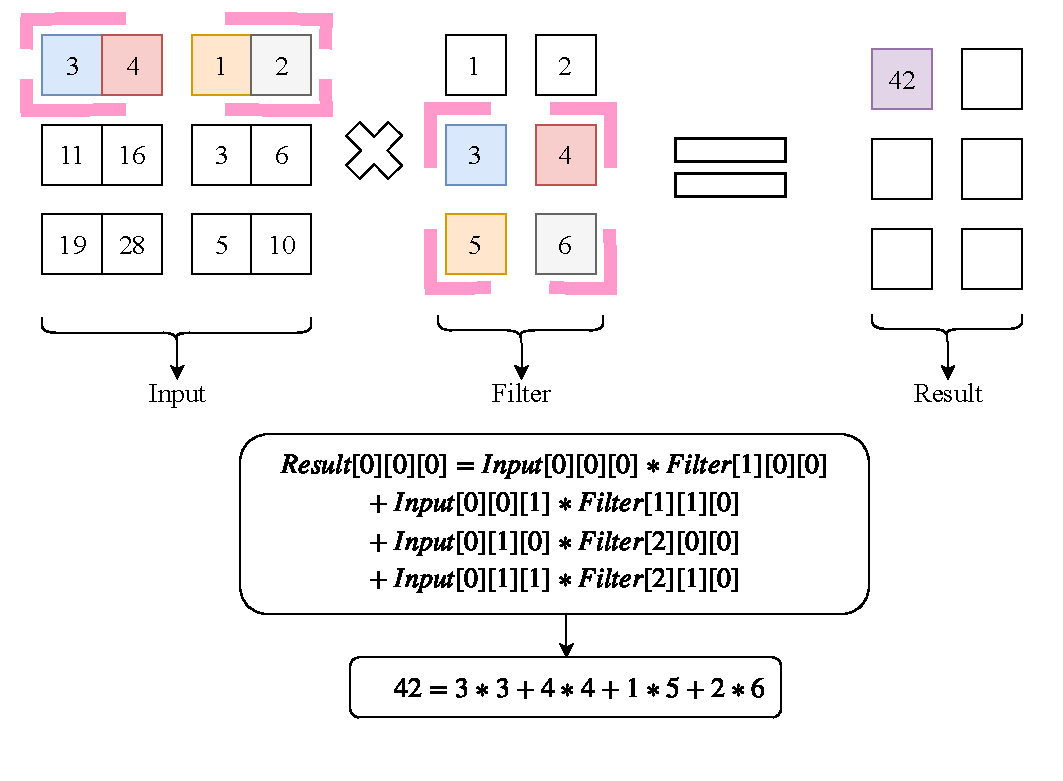
\includegraphics[width=0.9\textwidth]{secondConvSample_step1}
	\end{center}
\end{blockfigure}
\begin{blockfigure}{Extracting the second value from the first sample in the data tensor to the feature map.}
	\begin{center}
		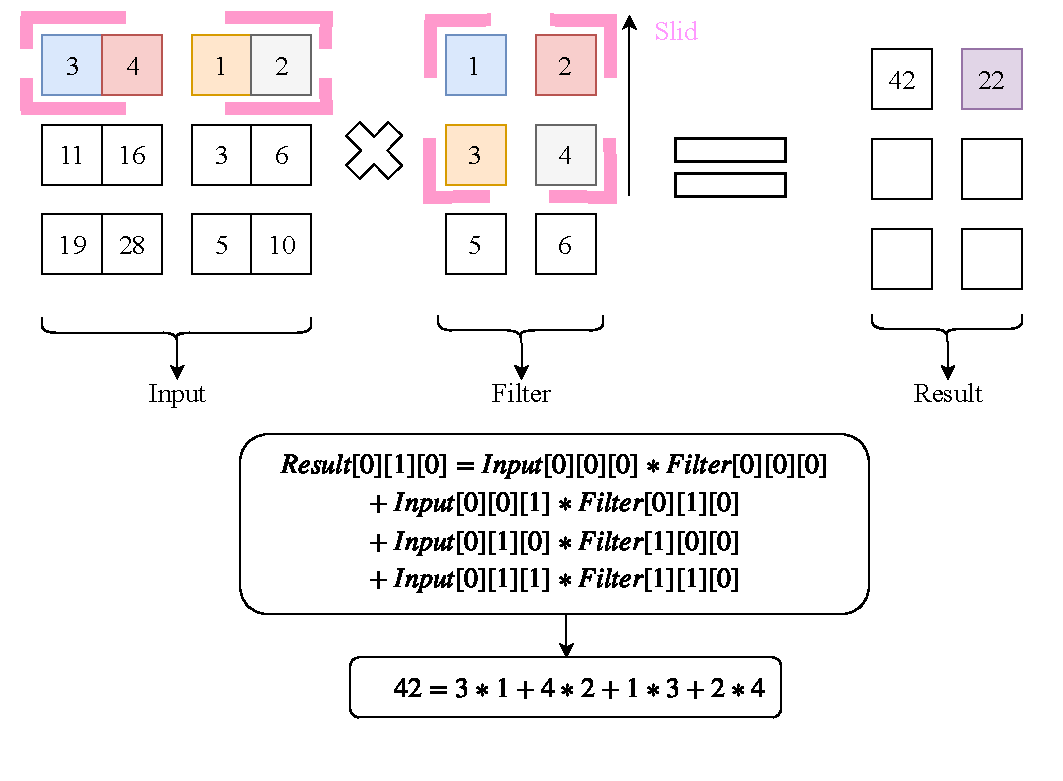
\includegraphics[width=0.9\textwidth]{secondConvSample_step2}
	\end{center}
\end{blockfigure}
\newpage
\begin{blockfigure}{The entire convolution performed on the data batch.}
	\begin{center}
		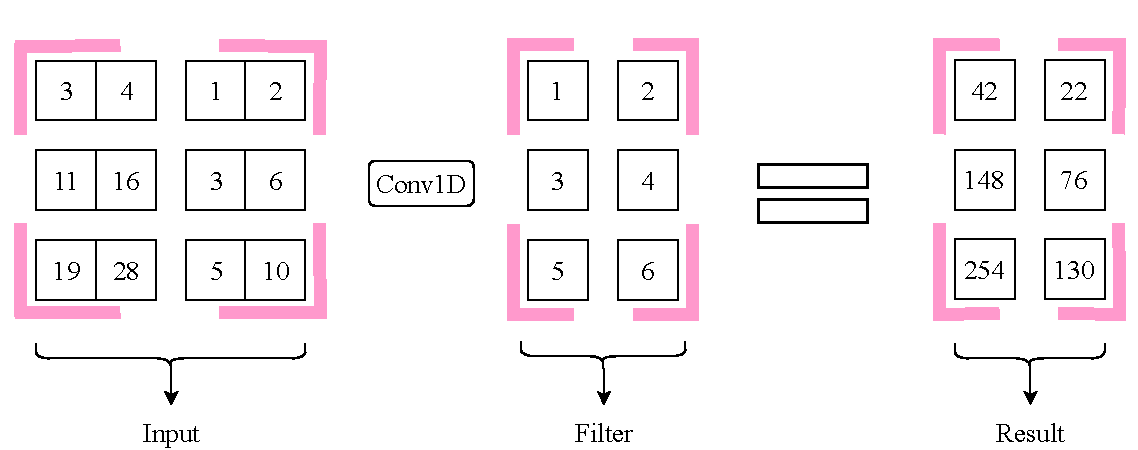
\includegraphics[width = \textwidth]{secondConvSample_final}
	\end{center}
\end{blockfigure}
\vspace{40pt}
From the final output we can conclude that the output 3D tensor is of shape (3, 2, 1), and it contains 1 feature maps, therefor it is similar in shape to the input tensor, as inferred previously in the example.
\vspace{40pt}
\begin{blockfigure}{squeezing of the z-axis onto the y-axis.}
	\begin{center}
		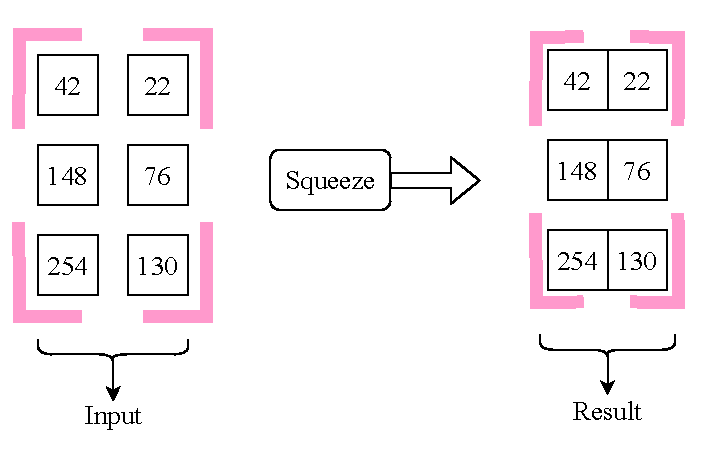
\includegraphics[width = \textwidth]{squeeze}
	\end{center}
\end{blockfigure}
\newpage
\section{\textbf{Batches}}
As seen from \cref{Conv1D}, when performing convolutions: we perform each convolution on each data sample separately.\\
Then the question arises: Why is a batch of samples needed?
The short answer is simply because a batch allows for a good experiment to take place from a statistical point of view.\\\\
When calculating the training error, each net performs mean reduction on each sample error, and a large sample is required for mean reduction (estimation), because the standard error of the mean ($ SEM $) can be expressed as:\\
\begin{center}
	\begin{minipage}{0.5\textwidth}
	$ SEM = \dfrac{\sigma}{\sqrt{n}} $\\
	Where:\\
	\tab \space \space $ \sigma: $ the standard deviation of the batch \\
	\tab \space \space $ n: $ the size of the batch 
\end{minipage}
\end{center}
The larger the batch size is, the less the $ SEM $ value is, the more confidence is placed in the accuracy of the mean reduction (estimation) of training errors.
\section{\textbf{Activation Functions}}
While doing the experiments with the project code, three combinations of activation functions were contemplated, but only one produced good results empirically upon conducting the tests. These three choices were:
\begin{itemize}[nosep]
	\item $" Sigmoid \rightarrow LeakyRealu \rightarrow Sigmoid "$.
	\item $" Tanh \rightarrow LeakyRealu \rightarrow Tanh "$.
	\item $" Sigmoid \rightarrow LeakyRealu \rightarrow Tanh "$.
\end{itemize}
If we take a look at the "Graph Diagram for an Example Dummy ConvNet" on page.~\pageref{fig:SimpleNetDiagram}, we deduce the following:
\begin{itemize}[nosep]
	\item The combination of activation functions chosen is: $" Sigmoid \rightarrow LeakyRealu \rightarrow Tanh "$.
	\item Each function is fed the result of matrix multiplication operations (involving float weight values), therefor each function receives float values as input.
	\item Sigmoid and LeakyRelu results are then fed to next layers, therefor their results are multiplied by a distribution of float values.
	\item Tanh processes the results of the output layer, therefor its output remains unchanged.
\end{itemize}
As for why $" Sigmoid \rightarrow LeakyRealu \rightarrow Tanh "$ produced the desired results, a hypothesis is constructed then tested with both numerical analysis and a suggested theoretical proof.
\begin{hypothesis}\label{hypothesis:1}
	the net can be considered as an information channel, and Shannon's theory \citep{Shannon:2001:MTC:584091.584093} applies to it, specially his entropy (on discrete values).
\end{hypothesis}
\begin{numericalanalysis}\label{analysis:1}
	considering a float distribution over an input x-axis, the distribution of possible result values over the y-axis can be described as the following:
\end{numericalanalysis}
\begin{itemize}[nosep]
	\item For $ Sigmoid \rightarrow LeakyRealu \rightarrow Sigmoid $:\\\tab $ \forall x \in X, X = [-1, +1]: Y = sigmoid(leakyRelu(sigmoid(X)*x)*x) $
	\item For $ Tanh \rightarrow LeakyRealu \rightarrow Tanh $:\\\tab $ \forall x \in X, X = [-1, +1]: Y = tanh(leakyRelu(tanh(X)*x)*x) $
	\item For $ Sigmoid \rightarrow LeakyRealu \rightarrow Tanh $:\\\tab $ \forall x \in X, X = [-1, +1]: Y = tanh(leakyRelu(sigmoid(X)*x)*x) $
\end{itemize}
\tab \tab  Where X is a line-space over the x-axis and Y is a line-space over the y-axis.
\begin{blockfigure} {$ \forall x \in X, X = [-1, +1] : Y = tanh(leakyRelu(tanh(X) * x) * x ) $}
	\begin{center}
		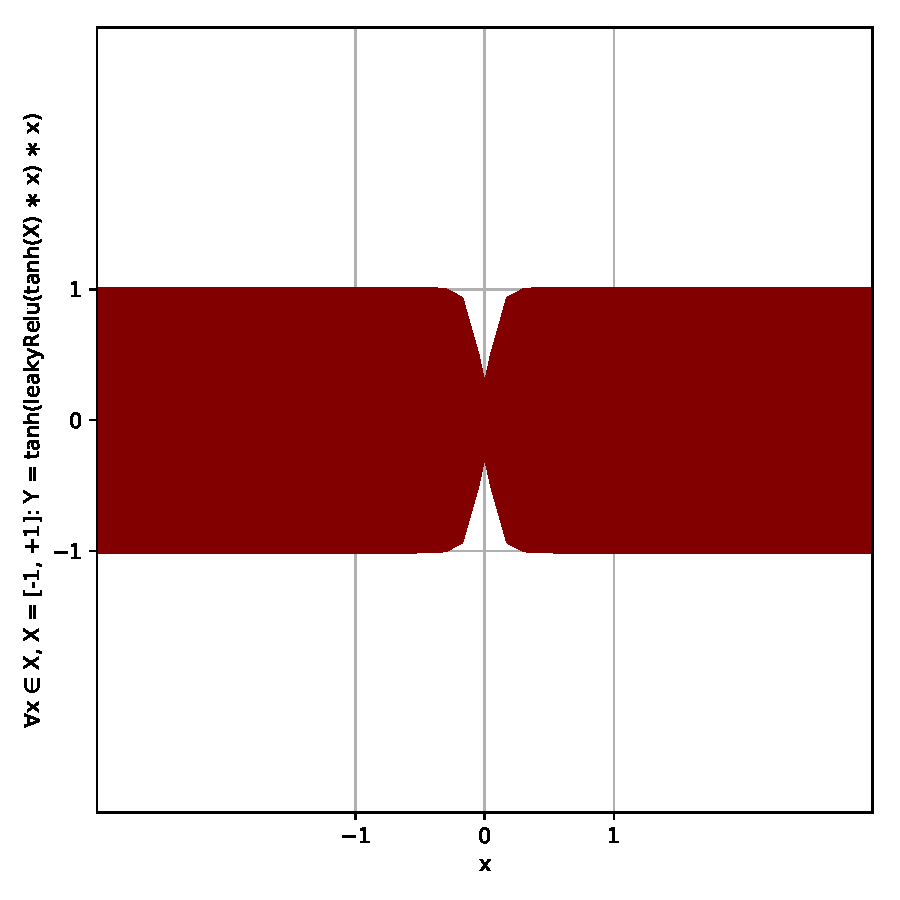
\includegraphics[width = 0.7\textwidth]{tanh_leakyRelu_tanh}
	\end{center}
\end{blockfigure}
\begin{blockfigure}{$ \forall x \in X, X = [-1, +1] : Y = sigmoid(leakyRelu(sigmoid(X) * x) * x) $}
	\begin{center}
		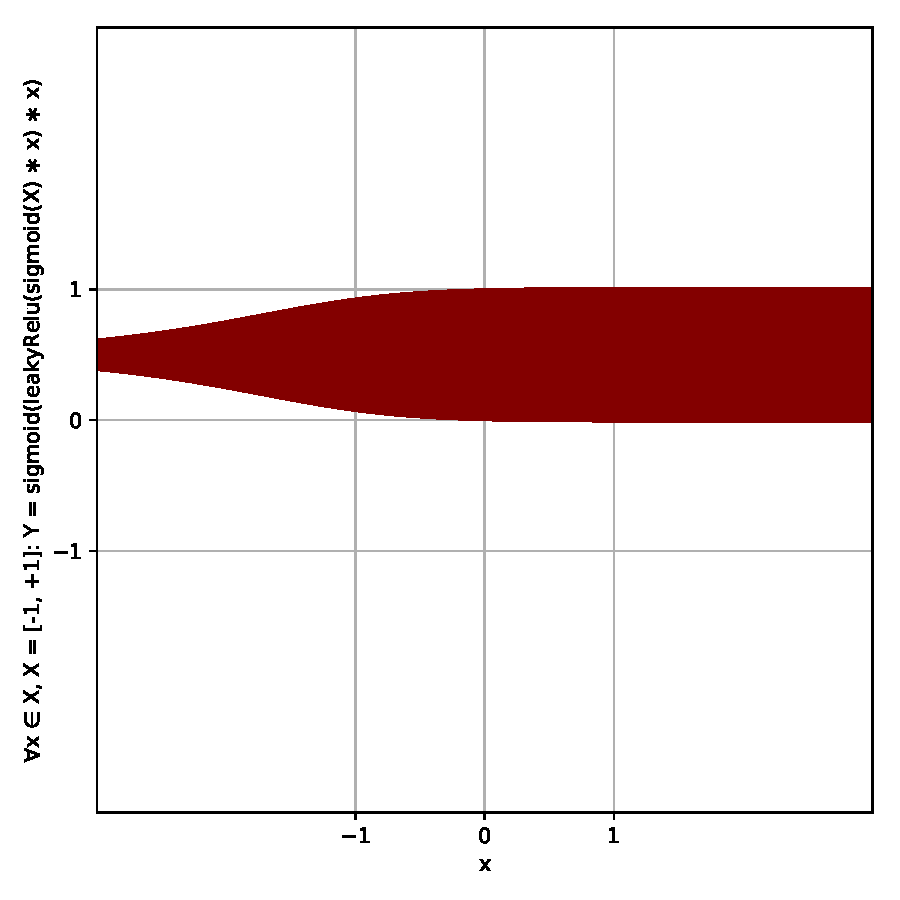
\includegraphics[width = 0.7\textwidth]{sigmoid_leakyRelu_sigmoid}
	\end{center}
\end{blockfigure}
\newpage
\begin{blockfigure}{$ \forall x \in X, X = [-1, +1] : Y = tanh(leakyRelu(sigmoid(X) * x) * x) $}
	\begin{center}
		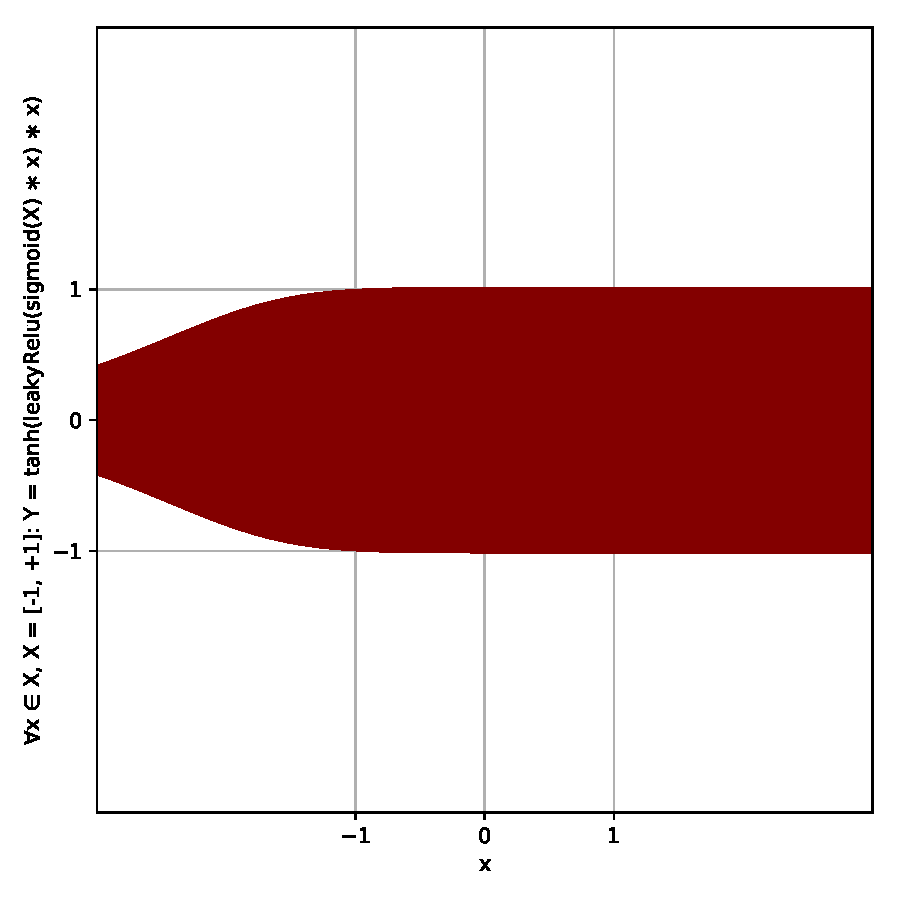
\includegraphics[width = 0.7\textwidth]{sigmoid_leakyRelu_tanh}
	\end{center}
\end{blockfigure}
\begin{suggestedproof}
	Shannon's entropy equation:
	\begin{center}
		$ H(V) = - \Sigma \space P(v_{i})*log_{b}(P(v_{i})) $
	\end{center}
	Since linespaces can be converted to discrete values, Shannon's entropy equation can be applied to the linespaces in Numerical-Analysis~\ref{analysis:1}, as the following:\\
	\begin{center}
		$ \forall x \in X, X = [-1, +1]: H(Y) = - \Sigma \space P(y_{i})*log_{b}(P(y_{i})) $
	\end{center}
	\begin{itemize}
		\item $" Sigmoid \rightarrow LeakyRealu \rightarrow Sigmoid "$ is equiprobable as we move along the x-axis, but it has less information capacity and therefor has a smaller $ H(Y) $ value.
		\item $" Tanh \rightarrow LeakyRealu \rightarrow Tanh "$ begins to become non-linearly inequiprobable as we move towards 0 along the x-axis, this not only results in less information capacity and a lower $ H(Y) $, but because each neuron in a layer is independent of the other, therefor each value probability along the x-axis is independent of the other, and the net could be training on a mix of values randomly chosen along the x-axis, this will lead to non-uniformality of information capacity and entropy across the trainable process (e.g. Conv1D), which will lead to inconsistent results for that process, and the convergence will jump up and down, and probably not get fully achieved.
		\item $" Sigmoid \rightarrow LeakyRealu \rightarrow Tanh "$ is equiprobable as we move along the x-axis, and it has more information capacity and therefor has a larger $ H(Y) $ value. 
	\end{itemize}
\end{suggestedproof}
\newpage
\section{\textbf{Loss Functions}}
\begin{definition}
	Loss functions are functions that map out the error of the network results compared to the desired output.
\end{definition}
The desired output for our nets are the following:
\begin{itemize}[nosep]
	\item For an Encryptor-Decryptor combination, loss has positive correlation with the arithmetic mean of the Encryptor-Decryptor losses, and negative correlation with the squared mean of the Eavesdropper losses:\\
	\tab $ Loss_{positive} = mean(Decryptor_{output} - Encryptor_{input}) $\\
	\tab $ Loss_{negative} = (1 - mean(Eavesdropper_{output} - Encryptor_{input}))^{2} $\\
	\tab $ Loss = Loss_{positive} + Loss_{negative} $
	\item For an Eavesdropper, loss has positive correlation with the arithmetic mean of the Eavesdropper losses, but is intended not to be aware of the losses of the Decryptor:\\
	\tab $ Loss = mean(Eavesdropper_{output} - Encryptor_{input}) $
\end{itemize}
\section{\textbf{Optimizers}}
\begin{definition}
	An Optimizer from an ANN perspective is an algorithm or a methodology used to optimize the weights of the net, in order for the net to converge on its local/global optima and effectively learn its designated task, the optimizer achieves this by reducing the error produced by the loss function(s).\\
	The optimizers employed in deep learning are generally stochastic, and they rely on back-propagation to deliver the calculated optimizations. 
\end{definition}
The state of the art in stochastic optimization that relies on back-propagation at this moment is the \textbf{Adam Optimizer} ~\citep{DBLP:journals/corr/KingmaB14}, which is out of the scope of this dissertation, mainly because it is a full topic in its own right, and it is well documented elsewhere, especially where it was proposed in its original paper.
\newpage
\chapter{Implementation}\label{sec:implementation}
\section{\textbf{Net Structures}}
The nets designed in this thesis are divided as the following:
\begin{itemize}
	\item Key Generators (in case of asymmetric schemes).
	\item Encryptors: Alice.
	\item Decryptors: Bob.
	\item Eavesdroppers: Alice (known adversary), Alan (unknown adversary).
\end{itemize}
Each of these nets share the following general sequential structure:
\begin{itemize}
	\item \textbf{Input Preprocessing:} either a concatenation of two related batches (key batch + message batch, key batch + cipher batch) on top of each other to produce an input batch, or just a pass through of an input batch (cipher batch passed through to Eve and Alan in case of symmetric cryptography, key batch passed through to the Key Generators in case of asymmetric cryptography).\\
	In case of concatenation, the final input shape becomes $ (512, 32) $, and in case of pass-through the final input shape becomes $ (512, 16) $.
	\item \textbf{Input Layer:} a series of sequential fully connected layers to teach the net about cryptanalysis, which is 1 layer in case of of: Alice, Bob, Key Generators, but for Eve and Alan it is: 
	\begin{center}
		$ \sum_{i = 0}^{i=n} No._{fcl}[i] $ ~ Where ~
		$ n \in [Alice, Bob, Key ~ Generators] $
	\end{center}
	That is to give both eavesdroppers an edge in cryptanalysis.\\
	The input layer(s) has a weight shape of $ (16 ~ or ~ 32, 32) $, which makes it normalize the shape of the data passed to the convolutional layer to become $ (512, 32) $.
	\item \textbf{Dimensionality Expansion:}  the shape of the data passed to the convolutional layer to become $ (512, 32, 1 $).
	\item \textbf{Convolutional Layers:} 4 layers, the first 3 has exactly one with stride 2 to reduce the shape of the data to $ (512, 16, 1) $ and they have leakyRelu as activation functions, the final layer has tanh as an activation function.
	\item \textbf{Output Layer:} reduces the dimensionality of the data to $ (512, 16) $ and gives it as an output batch. 
\end{itemize}
\newpage
\begin{blockfigure}{ Net Graph Diagram - Alice}
	\begin{center}
		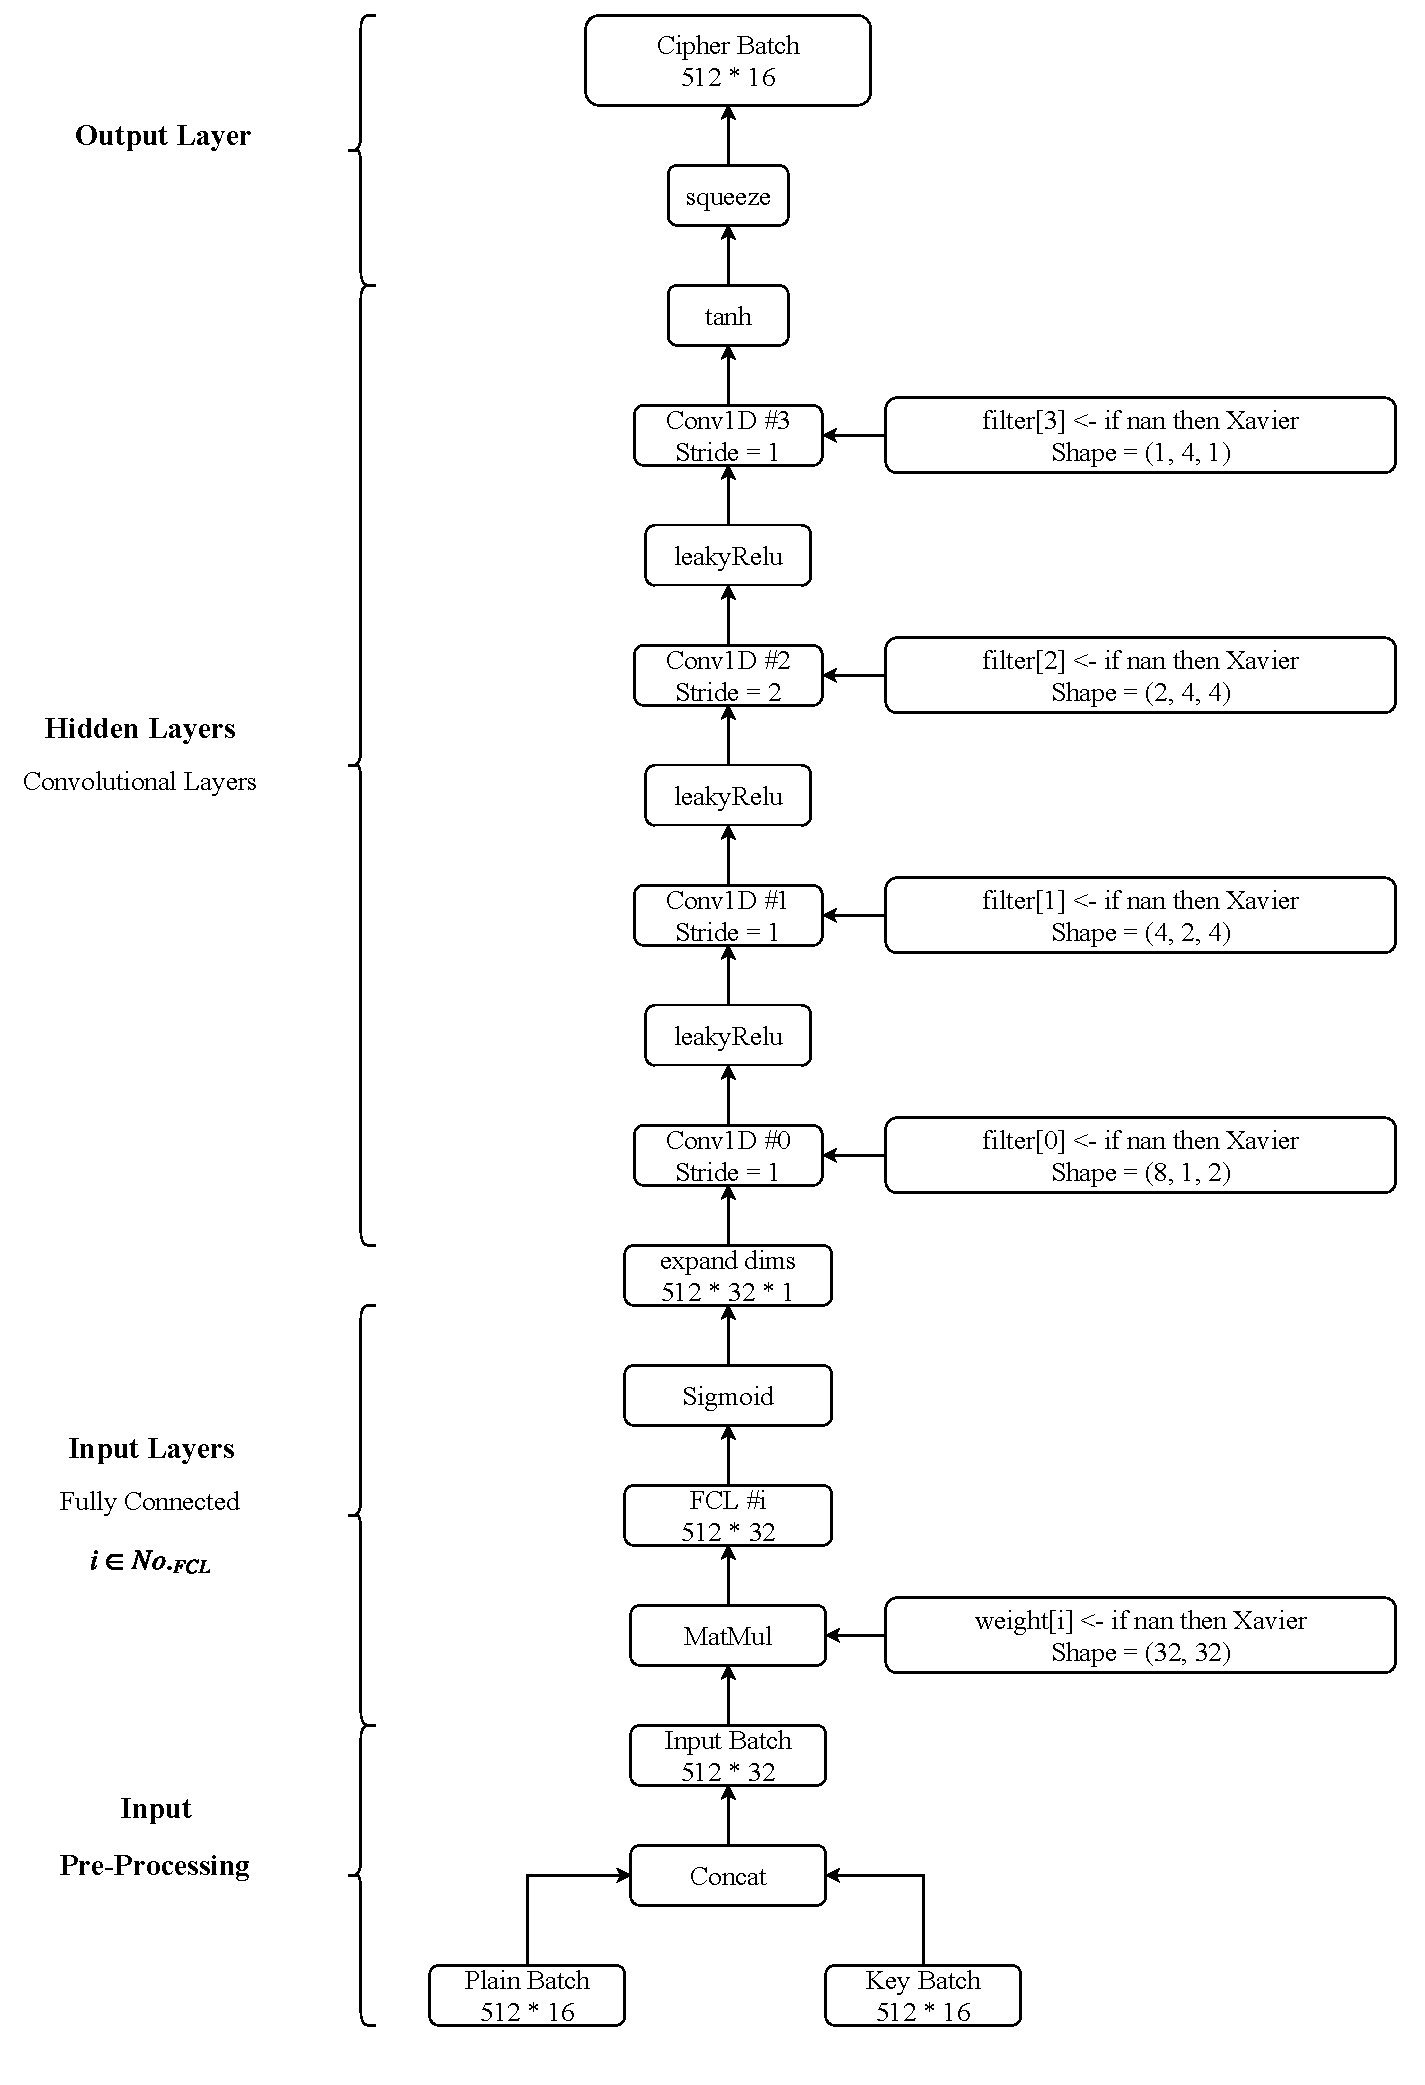
\includegraphics[width = \textwidth]{Alice-Diagram}
	\end{center}
\end{blockfigure}
\newpage
\begin{blockfigure}{ Net Graph Diagram - Bob}
	\begin{center}
		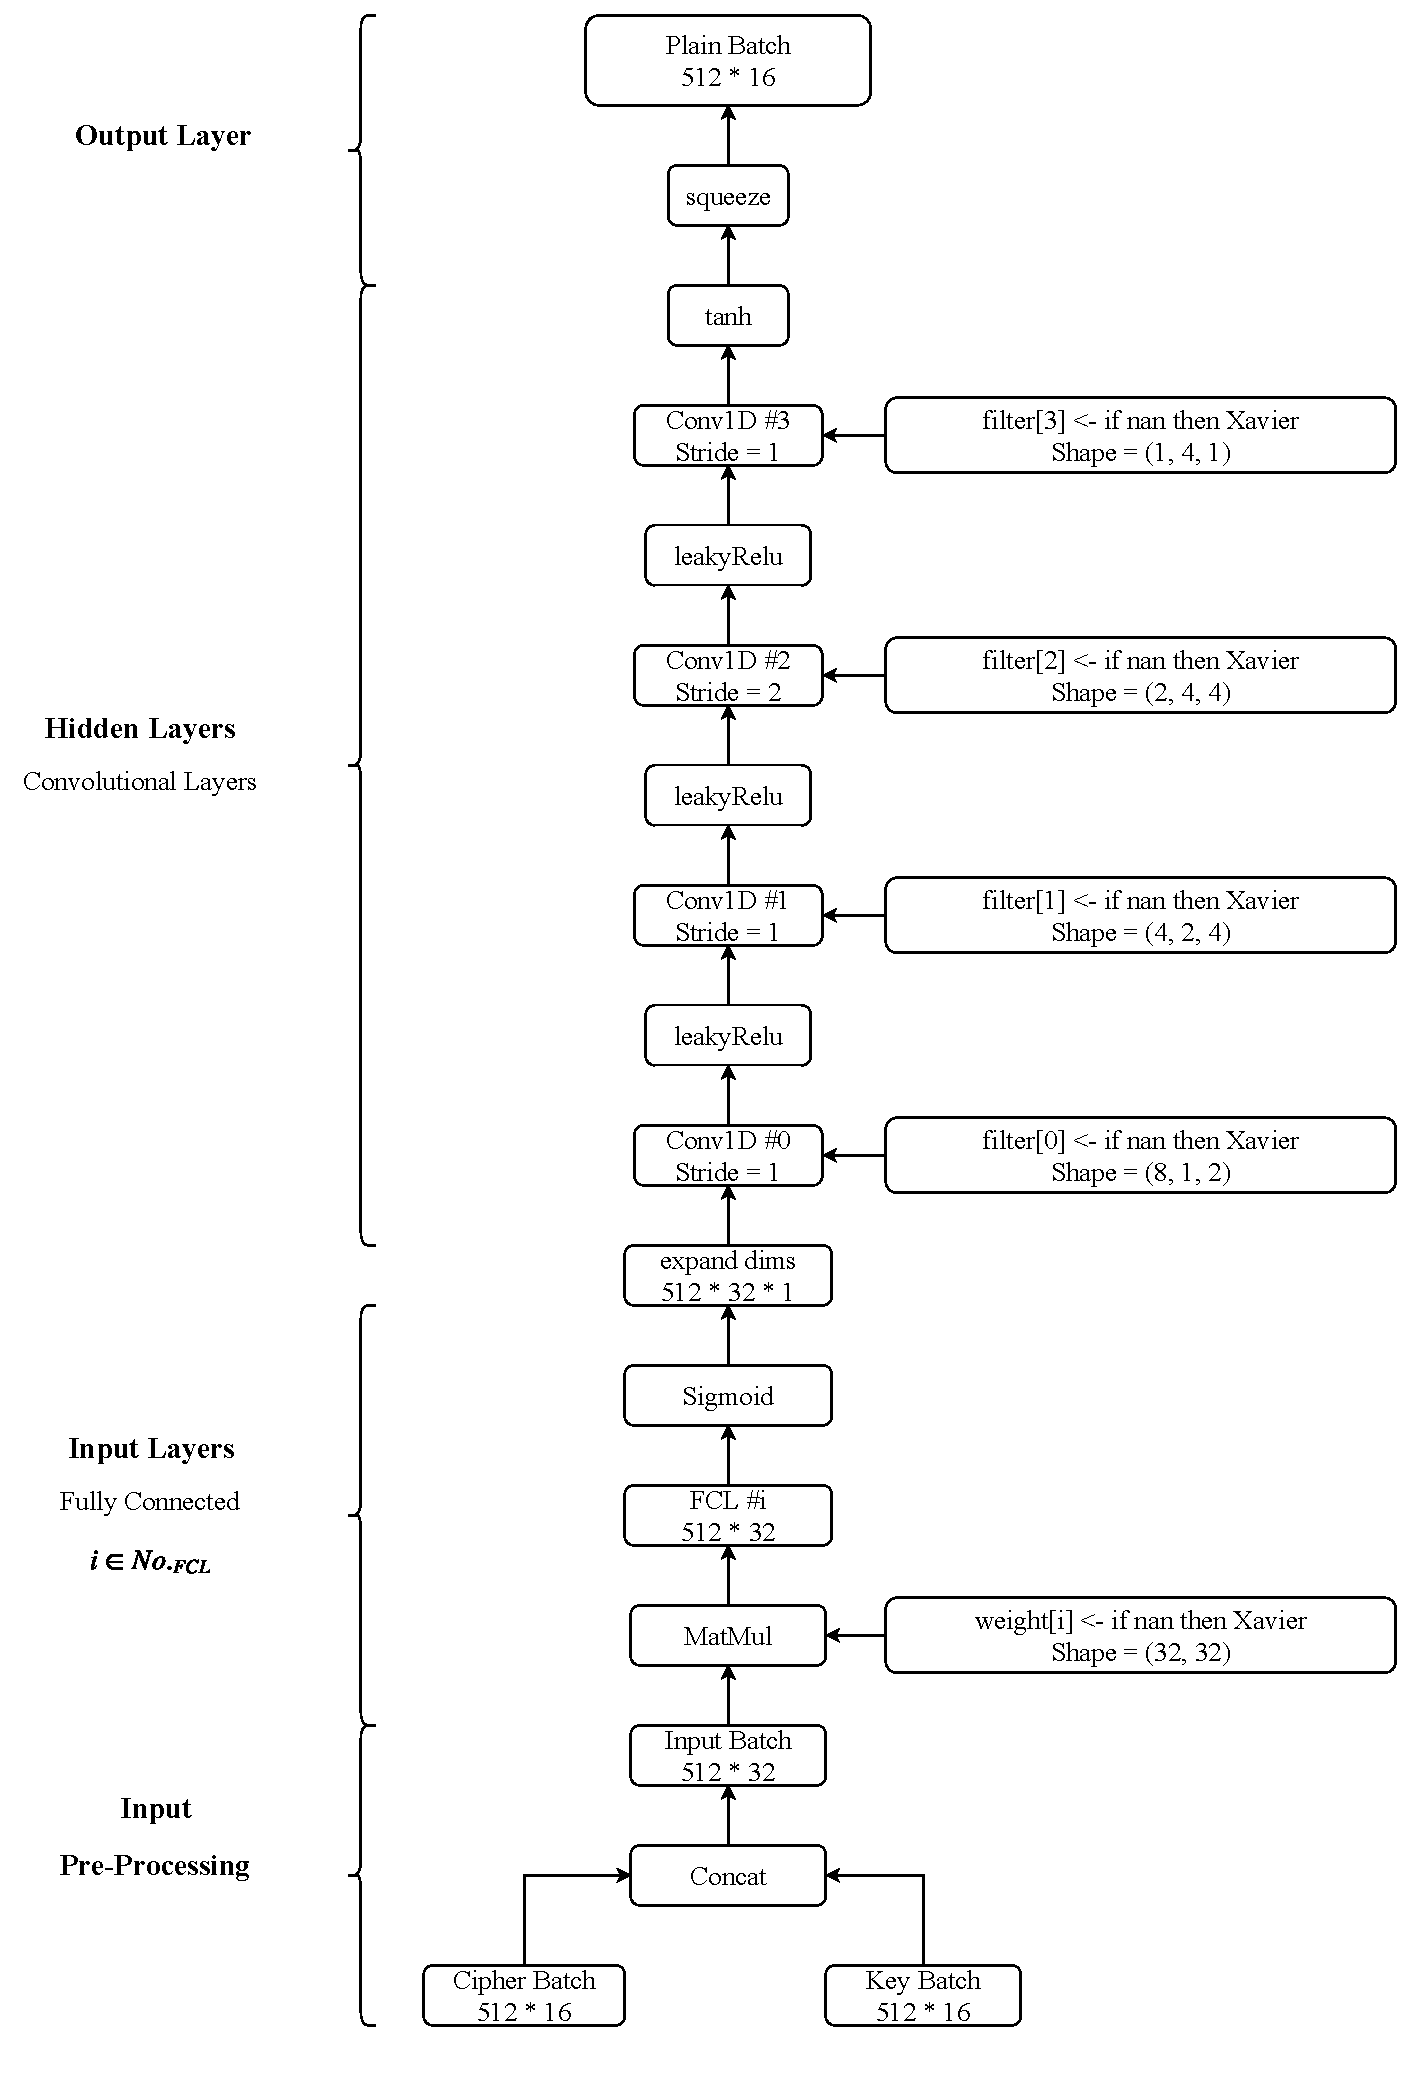
\includegraphics[width = \textwidth]{Bob-Diagram}
	\end{center}
\end{blockfigure}
\newpage
\begin{blockfigure}{ Net Graph Diagram - Eve/Alan}
		\begin{center}
			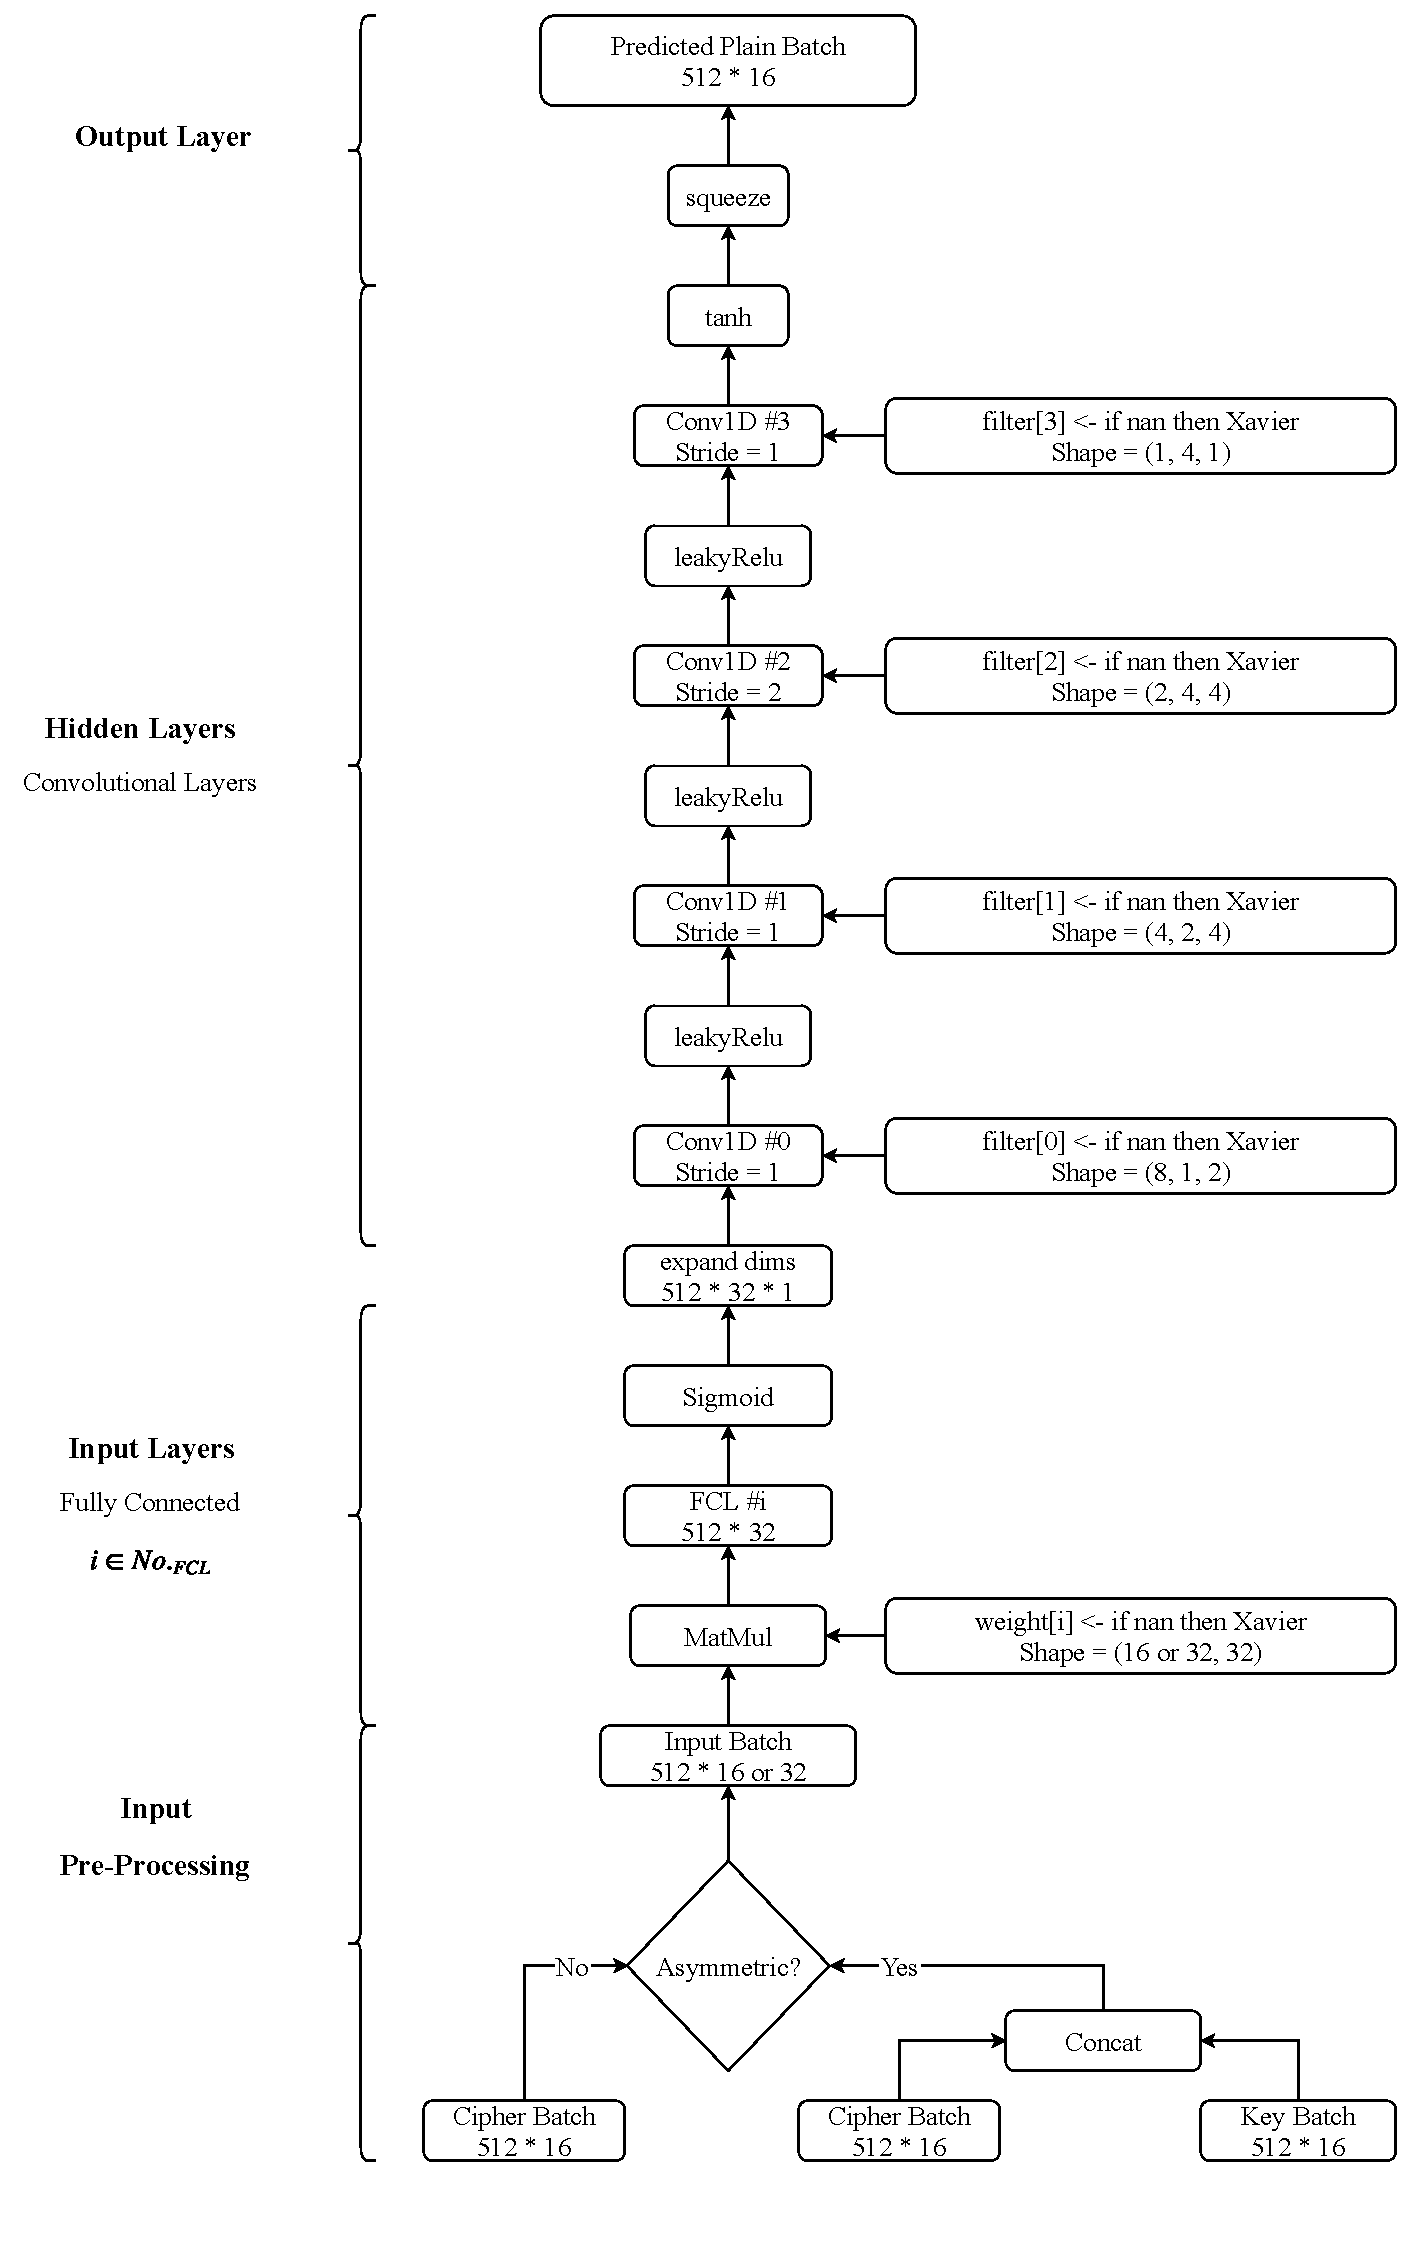
\includegraphics[width = \textwidth]{Eavesdropper-Diagram}
		\end{center}
\end{blockfigure}
\newpage
\begin{blockfigure}{ Net Graph Diagram - Key Generator}
	\begin{center}
		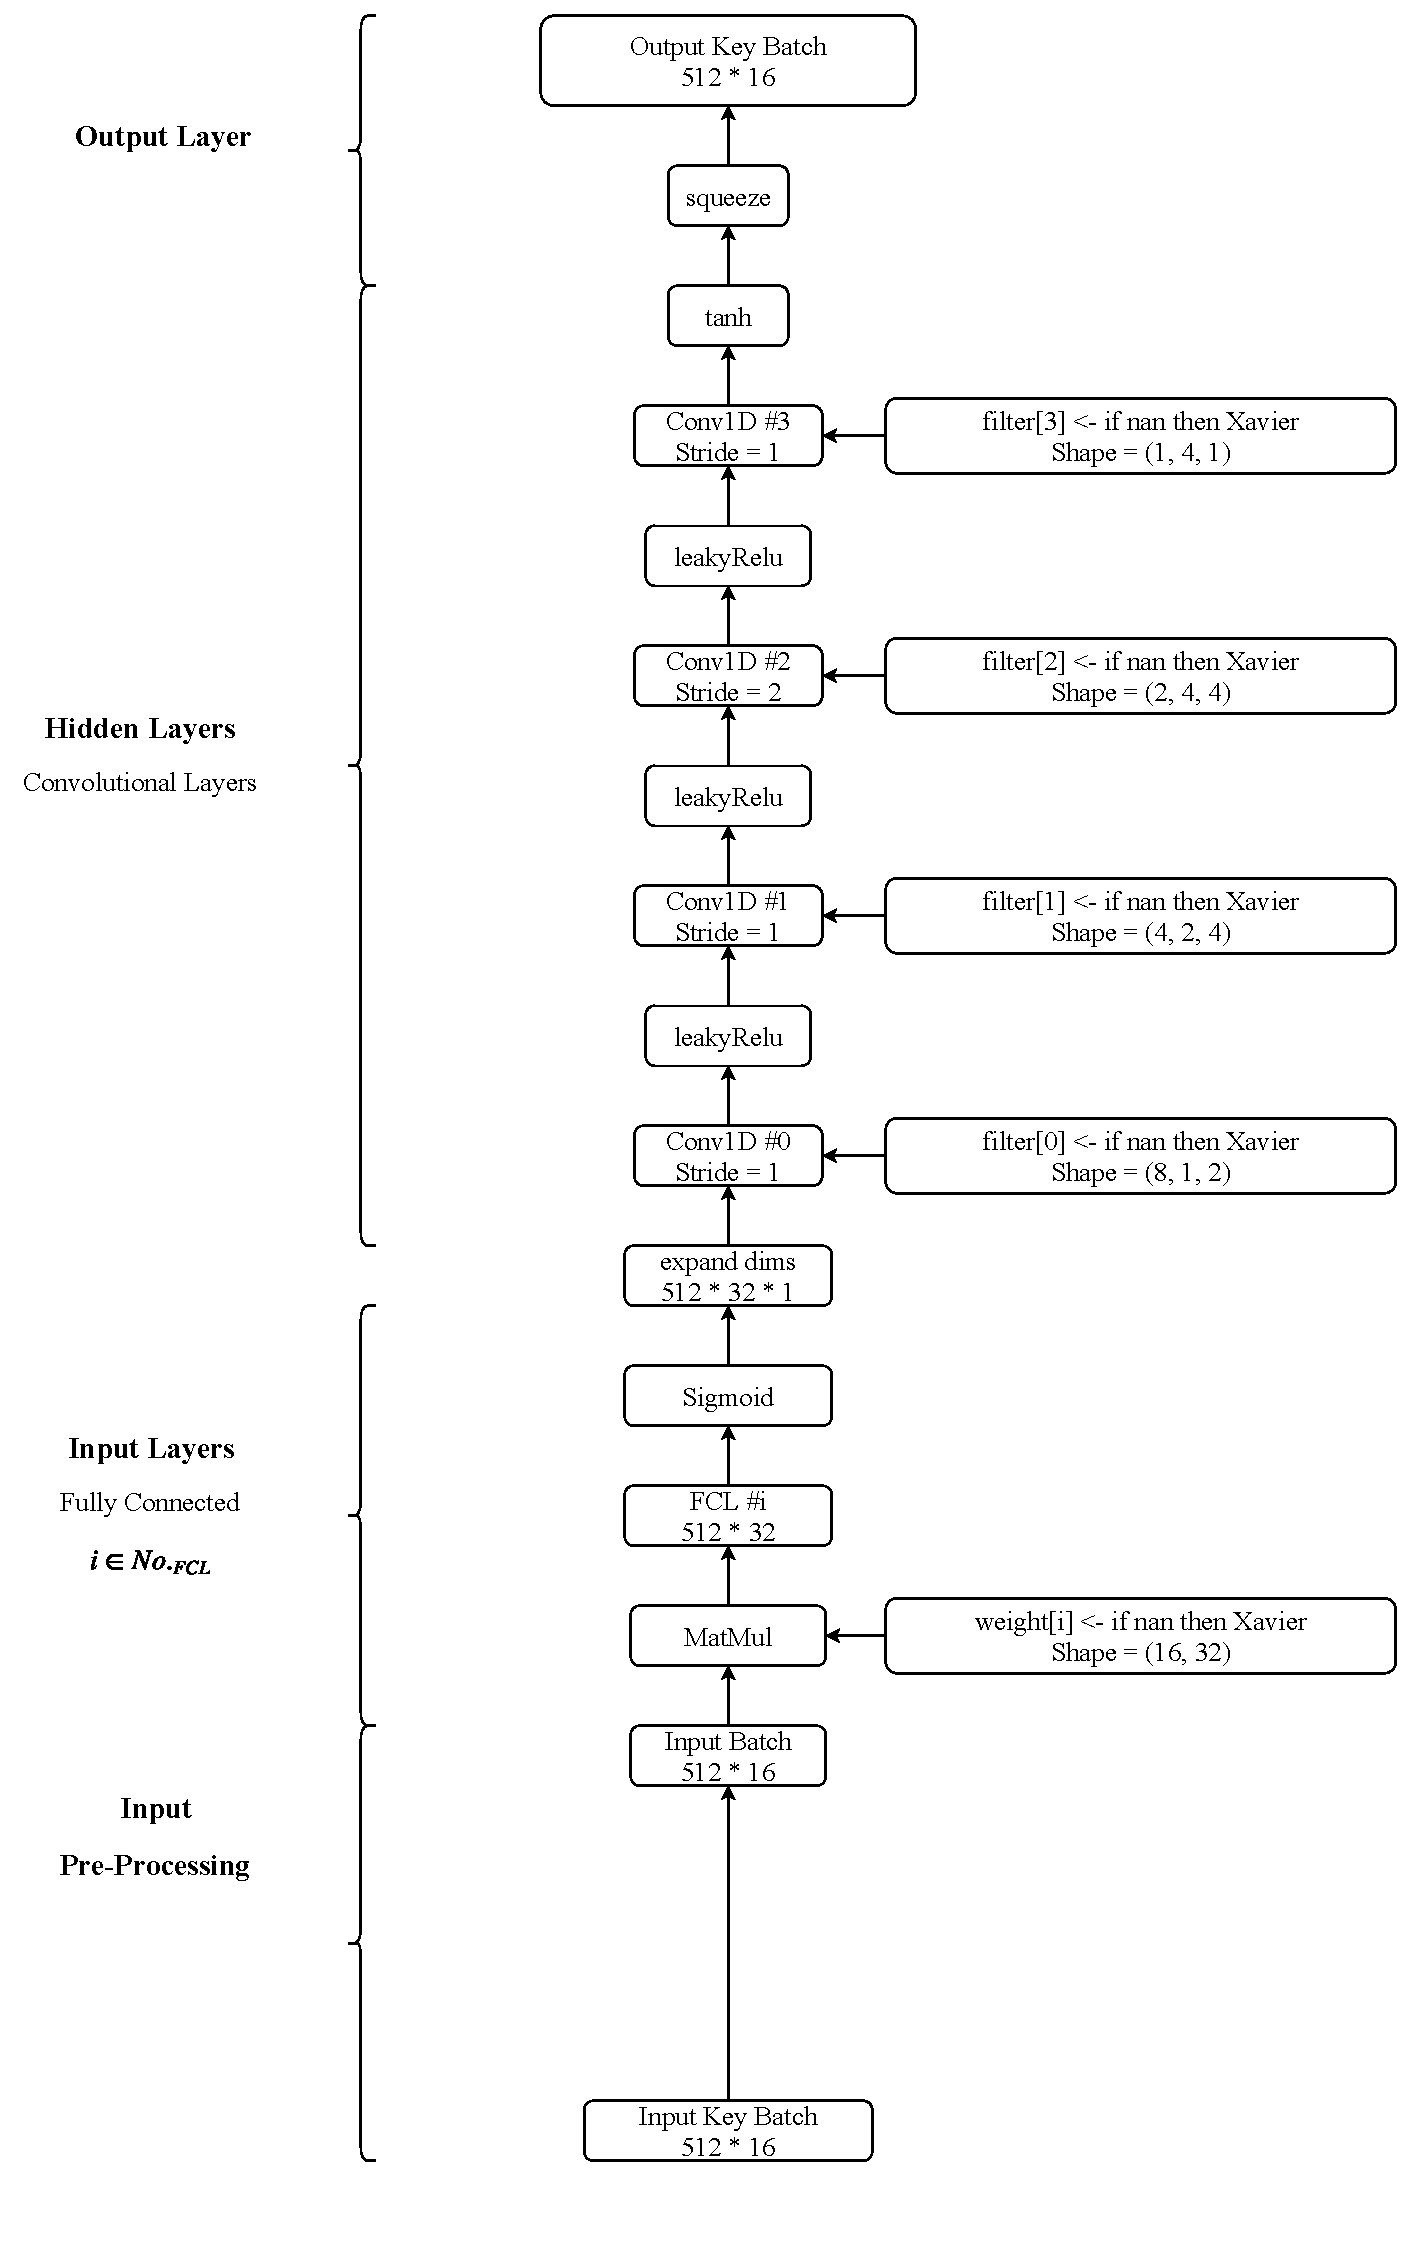
\includegraphics[width = \textwidth]{Generator-Diagram}
	\end{center}
\end{blockfigure}
\newpage
\section{\textbf{Scheme Structures}}
\subsection{\textbf{Symmetric Scheme}}
\paragraph{\textbf{Training}}\mbox{}\\
In the training setting, both Alice and Bob are fed the same key, Alice is fed the message (Plain) to be encrypted, then Alice sends the Cipher to Bob to decrypt it.
Both Eve and Alan intercept the Cipher from Alice and try to decrypt it without a key.
Every training iteration can be divided to three stages:
\begin{itemize}
	\item \textbf{Encryptor-Decryptor Stage:} Alice, Bob and Eve are activated.\\ both Bob and Eve try to decrypt the Cipher, then both their results get fed to the Encryptor-Decryptor (Alice-Bob) optimization process, only Alice and Bob get optimized at this stage, Eve plays a helpful adversary role, synonymous to a sparring partner for Alice and Bob.
	\item \textbf{Encryptor-Eavesdropper(Eve) Stage:} Alice and Eve are activated.\\ Alice encrypts, Eve intercepts and tries to decrypt, Eve's results get fed to the Eavesdropper (Eve) optimization process, only Eve gets optimized at this stage, in order to have a better adversary (a better sparring partner).
	\item \textbf{Encryptor-Eavesdropper(Alan) Stage:} Alice and Alan are activated.\\ Alice encrypts, Alan intercepts and tries to decrypt, Alan's results get fed to the Eavesdropper (Alan) optimization process, only Alan gets optimized at this stage, in order to have a malicious adversary, whom we don't know about, and who is a metric of how well the adversarial system performs in reality.
\end{itemize}
In the training setting, the Cipher is passed directly from the Encryptor to Bob, Eve and Alan, without being stored in between, because back-propagation does not work past static blocks of data (which is the case for stored Ciphers at the moment of back-propagation).\\
\paragraph{\textbf{Testing}}\mbox{}\\
In the testing setting, all neural nets are reconstructed with the same structures and with the same scheme in mind, the only difference is the lack of back-propagation in testing, and the need for a stored Cipher for a more production oriented system, which means the Cipher gets passed through an intermediate matrix instead of directly, from Alice to Bob, Eve and Alan.
\newpage
\begin{blockfigure}{ Symmetric Scheme}
	\begin{center}
		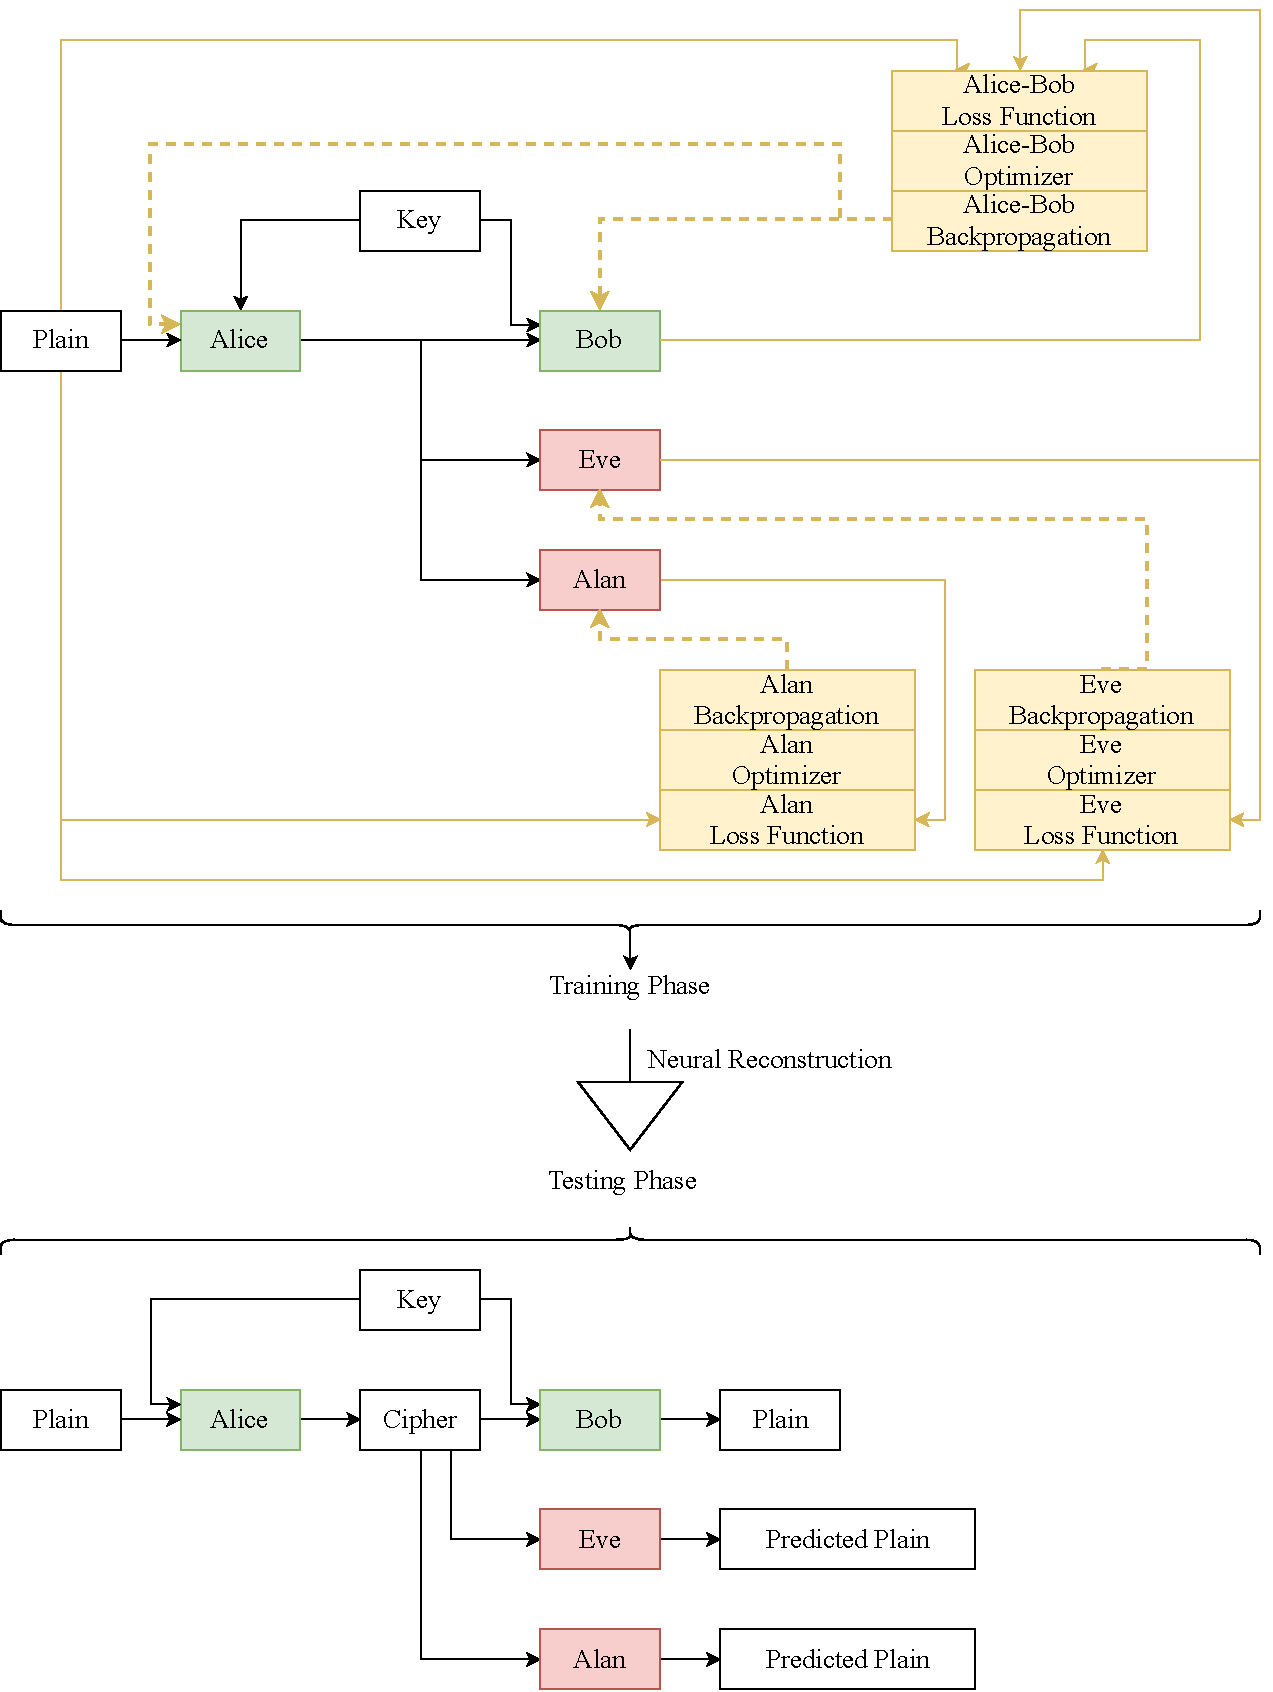
\includegraphics[width = \textwidth]{symmetricScheme}
	\end{center}
\end{blockfigure}
\newpage
\subsection{\textbf{Asymmetric Scheme}}
\paragraph{\textbf{Training}}\mbox{}\\
In the training setting:
\begin{itemize}
	\item The pubKey Generator is fed a key seed and produces a public key (pubKey).
	\item The privKey Generator is fed the pubKey and produces a private key (privKey).
	\item Alice is fed the pubKey and the message (Plain) and produces a Cipher.
	\item Bob is fed the privKey and the Cipher and tries to decrypt it.
	\item Both Eve and Alan intercept the Cipher from Alice and try to decrypt it with the pubKey.
\end{itemize}
Every training iteration can be divided to three stages:
\begin{itemize}
	\item \textbf{Encryptor-Decryptor Stage:} the pubKey Generator, the privKey Generator, Alice, Bob and Eve are activated.\\ both Bob and Eve try to decrypt the Cipher, then both their results get fed to the Encryptor-Decryptor (Alice-Bob) optimization process, only the pubKey Generator, the privKey Generator, Alice and Bob get optimized at this stage, Eve plays a helpful adversary role, synonymous to a sparring partner for Alice, Bob, the pubKey Generator and the privKey Generator.
	\item \textbf{Encryptor-Eavesdropper(Eve) Stage:} the pubKey Generator, the privKey Generator, Alice and Eve are activated.\\ Alice encrypts, Eve intercepts and tries to decrypt, Eve's results get fed to the Eavesdropper (Eve) optimization process, only Eve gets optimized at this stage, in order to have a better adversary (a better sparring partner).
	\item \textbf{Encryptor-Eavesdropper(Alan) Stage:} the pubKey Generator, the privKey Generator, Alice and Alan are activated.\\ Alice encrypts, Alan intercepts and tries to decrypt, Alan's results get fed to the Eavesdropper (Alan) optimization process, only Alan gets optimized at this stage, in order to have a malicious adversary, whom we don't know about, and who is a metric of how well the adversarial system performs in reality.
\end{itemize}
In the training setting, the Cipher is passed directly from the Encryptor to Bob, Eve and Alan, without being stored in between, because back-propagation does not work past static blocks of data (which is the case for stored Ciphers at the moment of back-propagation).
The same goes for the privKey-pubKey pair: 
\begin{itemize}
	\item The pubKey is passed directly to the privKey Generator, Alice, Eve and Alan without being stored.
	\item The privKey is passed directly from the privKey Generator to Bob without being stored.
\end{itemize}
Because we need back-propagation to reach the pubKey Generator and the privKey generator while training.
\paragraph{\textbf{Testing}}\mbox{}\\
In the testing setting, all neural nets are reconstructed with the same structures and with the same scheme in mind, the only difference is the lack of back-propagation in testing, and the need for a stored Cipher and a stored pubKey-privKey pair, for a more production oriented system. Which means: 
\begin{itemize}
	\item The Cipher gets passed through an intermediate matrix instead of directly, from Alice to Bob, Eve and Alan.
	\item The pubKey gets passed through an intermediate matrix instead of directly, to the privKey Generator, Alice, Eve and Alan.
	\item The privKey gets passed through an intermediate matrix instead of directly, from the privKey Generator to Bob.
\end{itemize}
\newpage
\begin{inlinefigure}{ Asymmetric Scheme}
	\begin{center}
		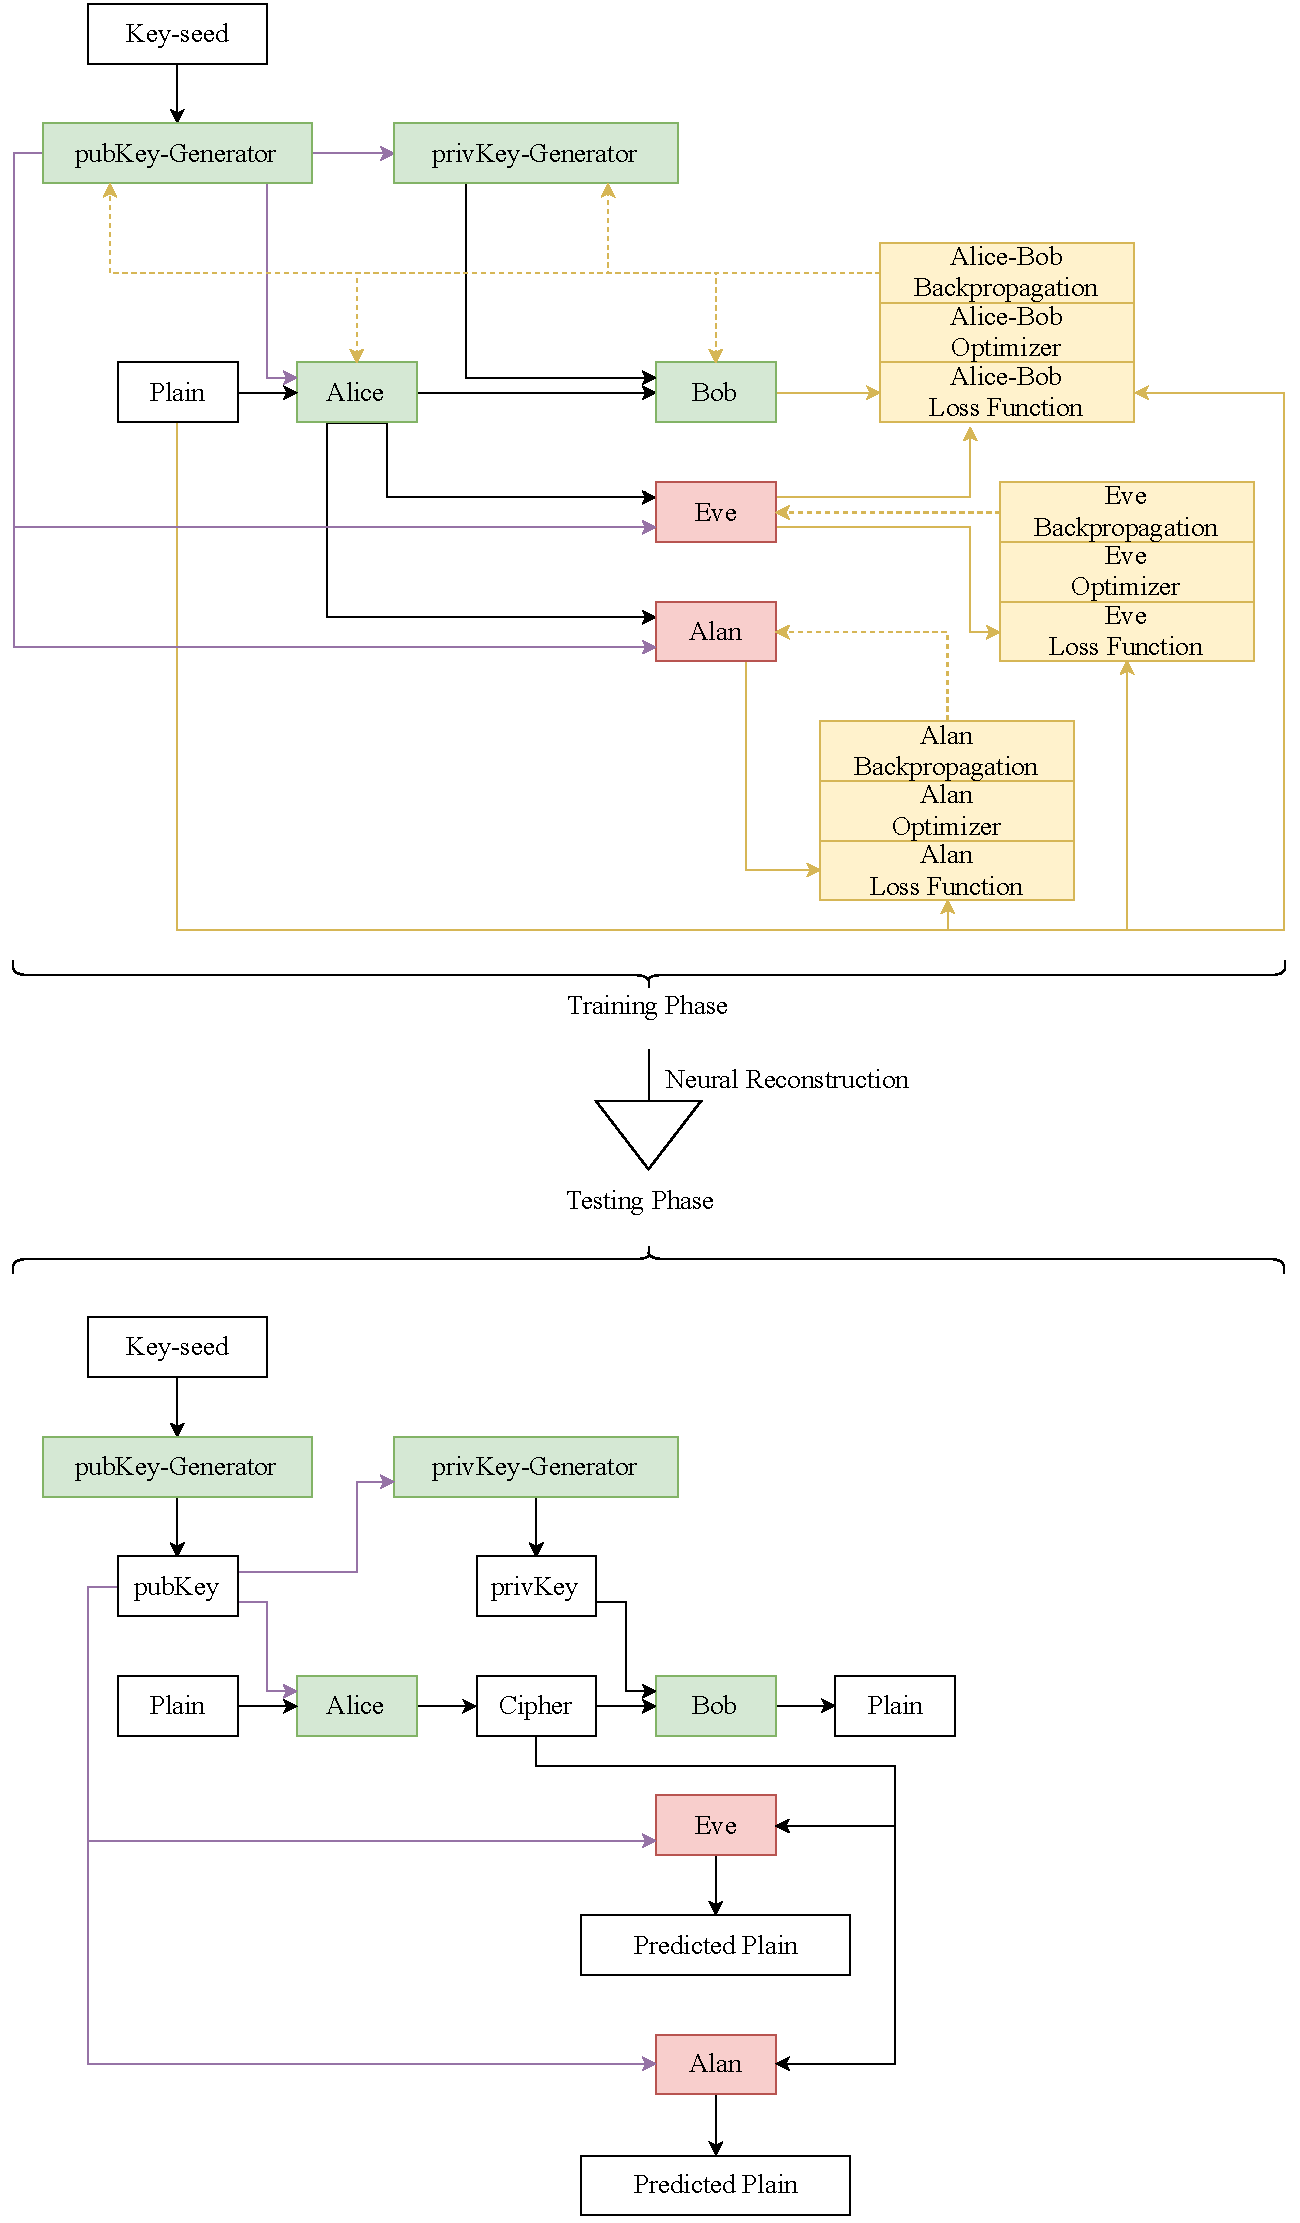
\includegraphics[width = \textwidth, height = 0.98\textheight]{asymmetricScheme}
	\end{center}
\end{inlinefigure}
\newpage
\subsection{\textbf{Hybrid Scheme}}
The idea behind this scheme is to use one scheme (asymmetric) in training, and another scheme (symmetric) in testing, and the aim is to bring the performance of the symmetric scheme to closely match that of the asymmetric scheme, the method behind such reconstruction from an asymmetric-trained graph to a symmetric-trained graph is called transfer learning.
\begin{definition}\label{definition:\thedefinition}
	(Transfer Learning): Given a source domain $ D_{S} $
	and learning task $ T_{S} $ , a target domain $ D_{T} $ and learning task
	$ T_{T} $ , transfer learning aims to help improve the learning of the
	target predictive function $ f_{T}(\cdot) $ in $ D_{T} $ using the knowledge in
	$ D_{S} $ and $ T_{S} $ , where $ D_{S} \neq D_{T} $ , or $ T_{S} \neq T_{T} $.~\citep{5288526}
\end{definition}
\paragraph{\textbf{Transfer Learning}}\mbox{}\\
From definition \ref{definition:\thedefinition}, we consider ~$ D = \{X , P (X)\} $, with $ X $ representing the data sets, and $ P(X) $ representing the predictions:
\begin{itemize}[nosep]
	\item $ \textbf{X} $\textbf{:} the data sets (key batch, plain-message batch) and (key-seed batch, plain-message batch) are the same, in the sense that they have the same sizes and they are both randomly generated, they also both follow the same normalized binary format (-1, 1).
	\item $ \textbf{P(X)} $\textbf{:} is also the same for both schemes from an intuitive standpoint, since both symmetric and asymmetric schemes produce predictions of the plain message that are of the same batch size, and are floating point values distributed between -1 and 1, but since we don't yet have statistical data on how they are distributed, this point needs to be further studied.
\end{itemize}
Also from definition \ref{definition:\thedefinition}, we consider ~$ T = \{Y, P(Y|X)\} $, with $ Y_{S} $, $ Y_{T} $ representing the label spaces, and $ P(Y|X) $ representing the conditional probability distributions:
\begin{itemize}[nosep]
	\item $ \boldsymbol{Y_{S}} $\textbf{,} $ \boldsymbol{Y_{T}} $\textbf{:} are equal since the source label space (asymmetric) is the same as the target label space (symmetric), in the sense that they both deal with (plain, key) labels as input and (predicted-plain) labels as output.
	\item $ \boldsymbol{P(Y|X)} $\textbf{:} differs between the two schemes from an intuitive standpoint, that is the conditional probability distributions between the schemes are different, which is a point that also needs to be further studied.
\end{itemize}
\begin{conjecture}
	beside the reason why transfer learning applies to the hybrid system, a reason to why it works well may lie in the asymmetric-training stage's ability to provide trained weights that are derived from training on generated keys that come from a floating point distribution, as opposed to training on keys that are of normalized binary form in the symmetric-scheme training stage.
\end{conjecture}
\newpage
\paragraph{\textbf{Training}}\mbox{}\\
In the training setting:
\begin{itemize}
	\item The pubKey Generator is fed a key seed and produces a public key (pubKey).
	\item The privKey Generator is fed the pubKey and produces a private key (privKey).
	\item Alice is fed the pubKey and the message (Plain) and produces a Cipher.
	\item Bob is fed the privKey and the Cipher and tries to decrypt it.
	\item Both Eve and Alan intercept the Cipher from Alice and try to decrypt it without the pubKey.
\end{itemize}
Every training iteration can be divided to three stages:
\begin{itemize}
	\item \textbf{Encryptor-Decryptor Stage:} the pubKey Generator, the privKey Generator, Alice, Bob and Eve are activated.\\ both Bob and Eve try to decrypt the Cipher, then both their results get fed to the Encryptor-Decryptor (Alice-Bob) optimization process, only the pubKey Generator, the privKey Generator, Alice and Bob get optimized at this stage, Eve plays a helpful adversary role, synonymous to a sparring partner for Alice, Bob, the pubKey Generator and the privKey Generator.
	\item \textbf{Encryptor-Eavesdropper(Eve) Stage:} the pubKey Generator, the privKey Generator, Alice and Eve are activated.\\ Alice encrypts, Eve intercepts and tries to decrypt, Eve's results get fed to the Eavesdropper (Eve) optimization process, only Eve gets optimized at this stage, in order to have a better adversary (a better sparring partner).
	\item \textbf{Encryptor-Eavesdropper(Alan) Stage:} the pubKey Generator, the privKey Generator, Alice and Alan are activated.\\ Alice encrypts, Alan intercepts and tries to decrypt, Alan's results get fed to the Eavesdropper (Alan) optimization process, only Alan gets optimized at this stage, in order to have a malicious adversary, whom we don't know about, and who is a metric of how well the adversarial system performs in reality.
\end{itemize}
In the training setting, the Cipher is passed directly from the Encryptor to Bob, Eve and Alan, without being stored in between, because back-propagation does not work past static blocks of data (which is the case for stored Ciphers at the moment of back-propagation).
The same goes for the privKey-pubKey pair: 
\begin{itemize}
	\item The pubKey is passed directly to the privKey Generator \& Alice without being stored.
	\item The privKey is passed directly from the privKey Generator to Bob without being stored.
\end{itemize}
Because we need back-propagation to reach the pubKey Generator and the privKey generator while training.
\paragraph{\textbf{Testing}}\mbox{}\\
In the testing setting, all neural nets are reconstructed with the same structures and with the same scheme in mind, the only difference is the lack of back-propagation in testing, and the need for a stored Cipher and a stored pubKey-privKey pair, for a more production oriented system. Which means: 
\begin{itemize}
	\item The Cipher gets passed through an intermediate matrix instead of directly, from Alice to Bob, Eve and Alan.
	\item The pubKey gets passed through an intermediate matrix instead of directly, to the privKey Generator \& Alice.
	\item The privKey gets passed through an intermediate matrix instead of directly, from the privKey Generator to Bob.
\end{itemize}
\newpage
\begin{blockfigure}{ Hybrid Scheme}
	\begin{center}
		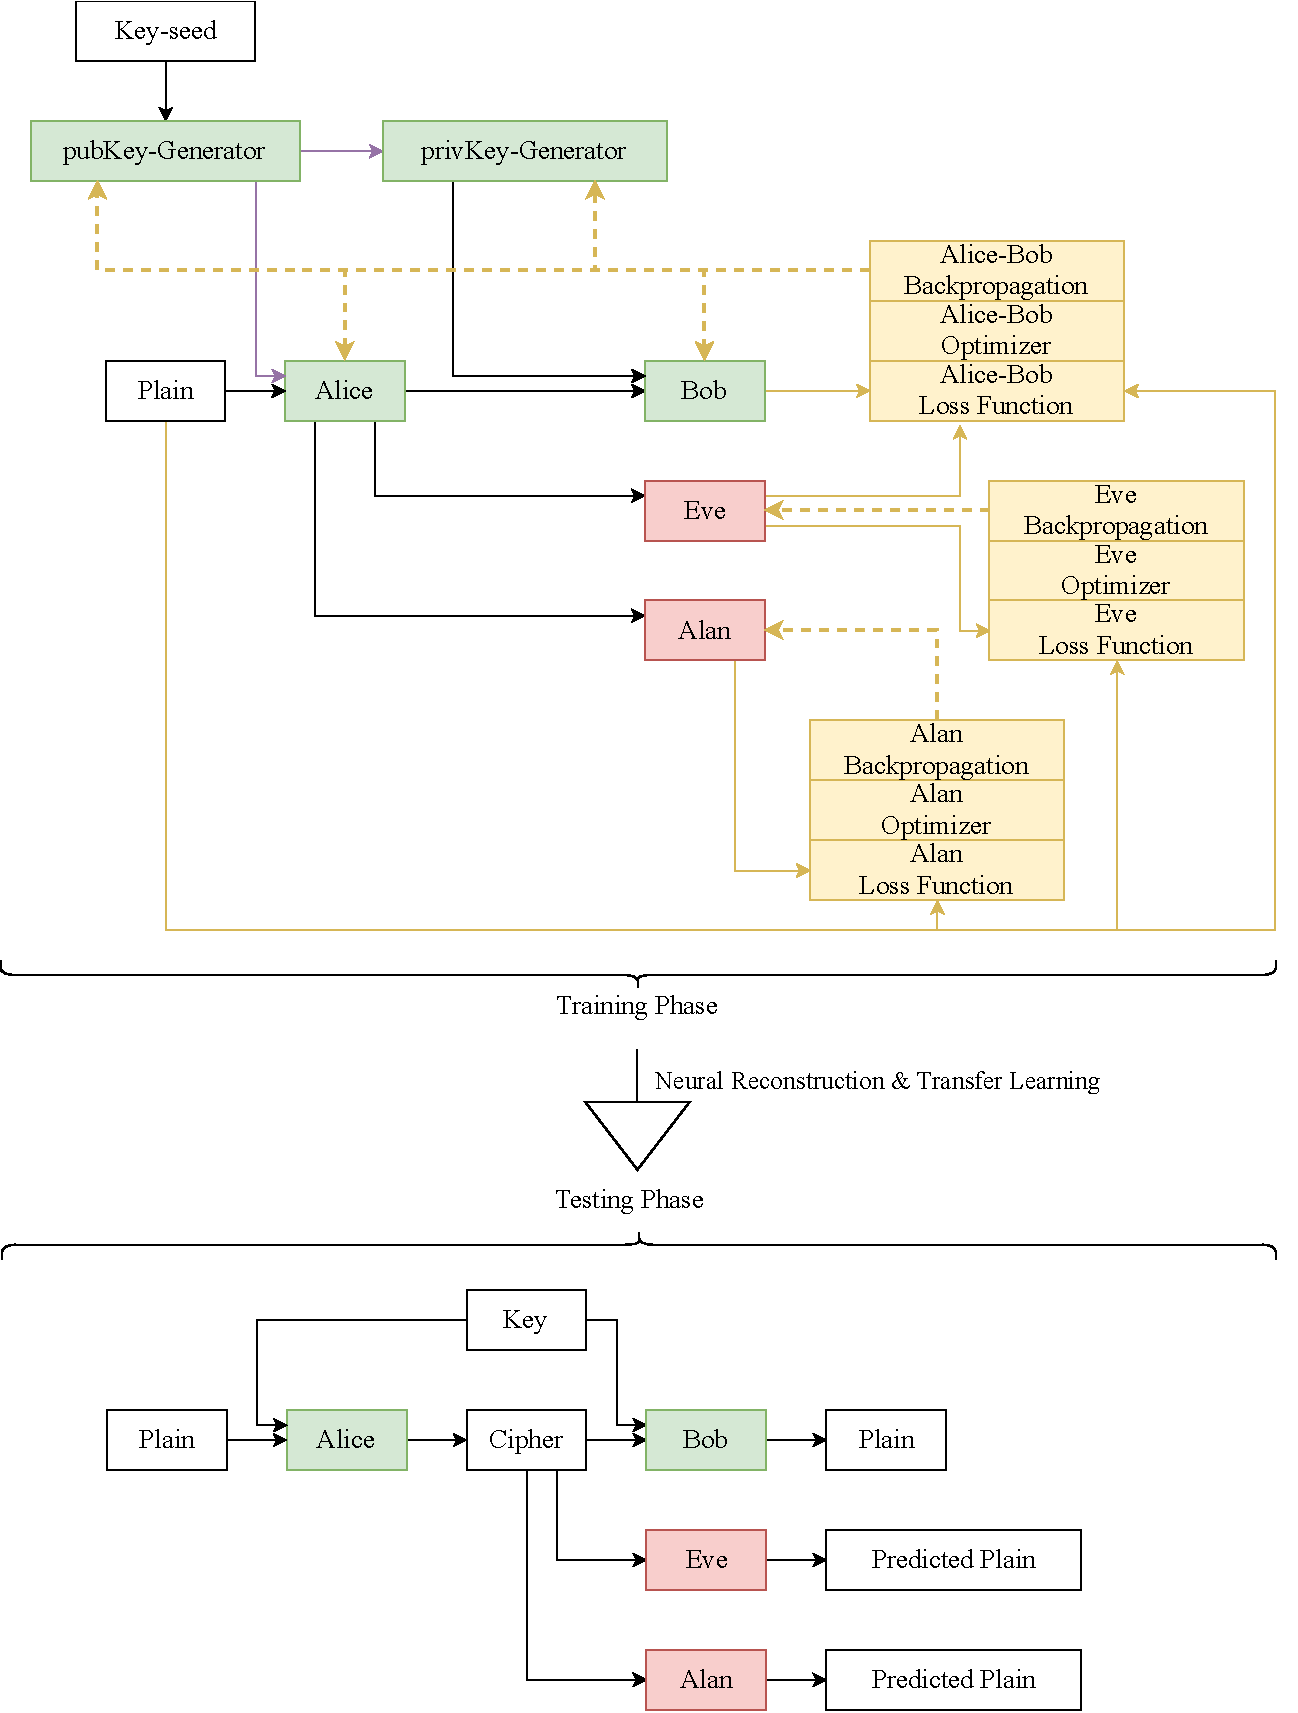
\includegraphics[width = \textwidth]{hybridScheme}
	\end{center}
\end{blockfigure}
\newpage
\section{\textbf{Project Structure}}
The schemes and the experiments they represent, presented in this thesis, were implemented with an object oriented design, methods that perform the exact same thing for all schemes were packed into one base class, the parameter loading was handled with one class, and the rest was implemented with different classes.\\
The following is a description of the common classes:\\
\begin{itemize}
	\item \textbf{general\_hyper\_parameters:} loads the hyper parameters stored in a json file, and performs checks on data that has to follow a certain format (e.g. filter shapes).
	\item \textbf{neurencoder\_base:} performs singular net building (not an entire scheme graph), training and result processing (e.g. display of errors accross iterations).
\end{itemize}
All schemes have the following common classes with the same overloaded/overriden methods:
\begin{itemize}
	\item \textbf{\%scheme\%\_hyper\_parameters:} adjusts the hyper parameters to be useful for the scheme (e.g. the number of FCL for eavesdroppers).
	\item \textbf{\%scheme\%\_training\_model:} builds an entire trainable graph for the scheme.
	\item \textbf{\%scheme\%\_testing\_model:} builds an entire testable graph for the scheme.
	\item \textbf{\%scheme\%\_model\_tester:} performs testing iterations on the scheme's testing model.
\end{itemize}
At the epicenter of all these classes, is the main class \textbf{\textit{neurencoder}}, which performs inheritance of the required classes for the scheme chosen by the user, then composes that scheme internally.\\
An exception to the common classes between schemes is the lack of a hybrid\_hyper\_parameters and a hybrid\_model\_tester, that is because the hybrid model is constructed as the following:
\begin{itemize}
	\item The hybrid scheme inherits from asymmetric\_hyper\_parameters, because it needs to train on asymmetric cryptography.
	\item The hybrid scheme inherits from symmetric\_model\_tester, because its testing model is re-built with symmetric cryptography in mind.
\end{itemize}
It is also expected after further development that the hybrid scheme will lose its hybrid\_training\_model and inherit the asymmetric\_training\_model instead.
\subsection{\textbf{Project Infrastructure}}
\begin{colortable}{Python Libraries Used in Core Functionality Development}
	\textbf{Name} & \textbf{Version} \\\hline
	sys & 3.5 \\\hline
	os & 3.5 \\\hline
	json & 3.5 \\\hline
	tensorflow & 1.8 \\\hline
	numpy & 1.14.2 \\\hline
	progressbar2 & 3.37.1 \\\hline
	matplotlib & 2.2.2 \\\hline
	seaborn & 0.8.1 \\\hline
	pyqtgraph & 0.10.0 \\\hline
	datetime & 4.2 \\\hline
\end{colortable}
\begin{colortable}{Python Libraries Used in Random Number Generation From Audio Sampling}
	\textbf{Name} & \textbf{Version} \\\hline
	sounddevice & 0.3.11 \\\hline
	hashlib & 3.5 \\\hline
\end{colortable}
\newpage
\begin{blockfigure}{Project Class Diagram}
	\begin{center}
		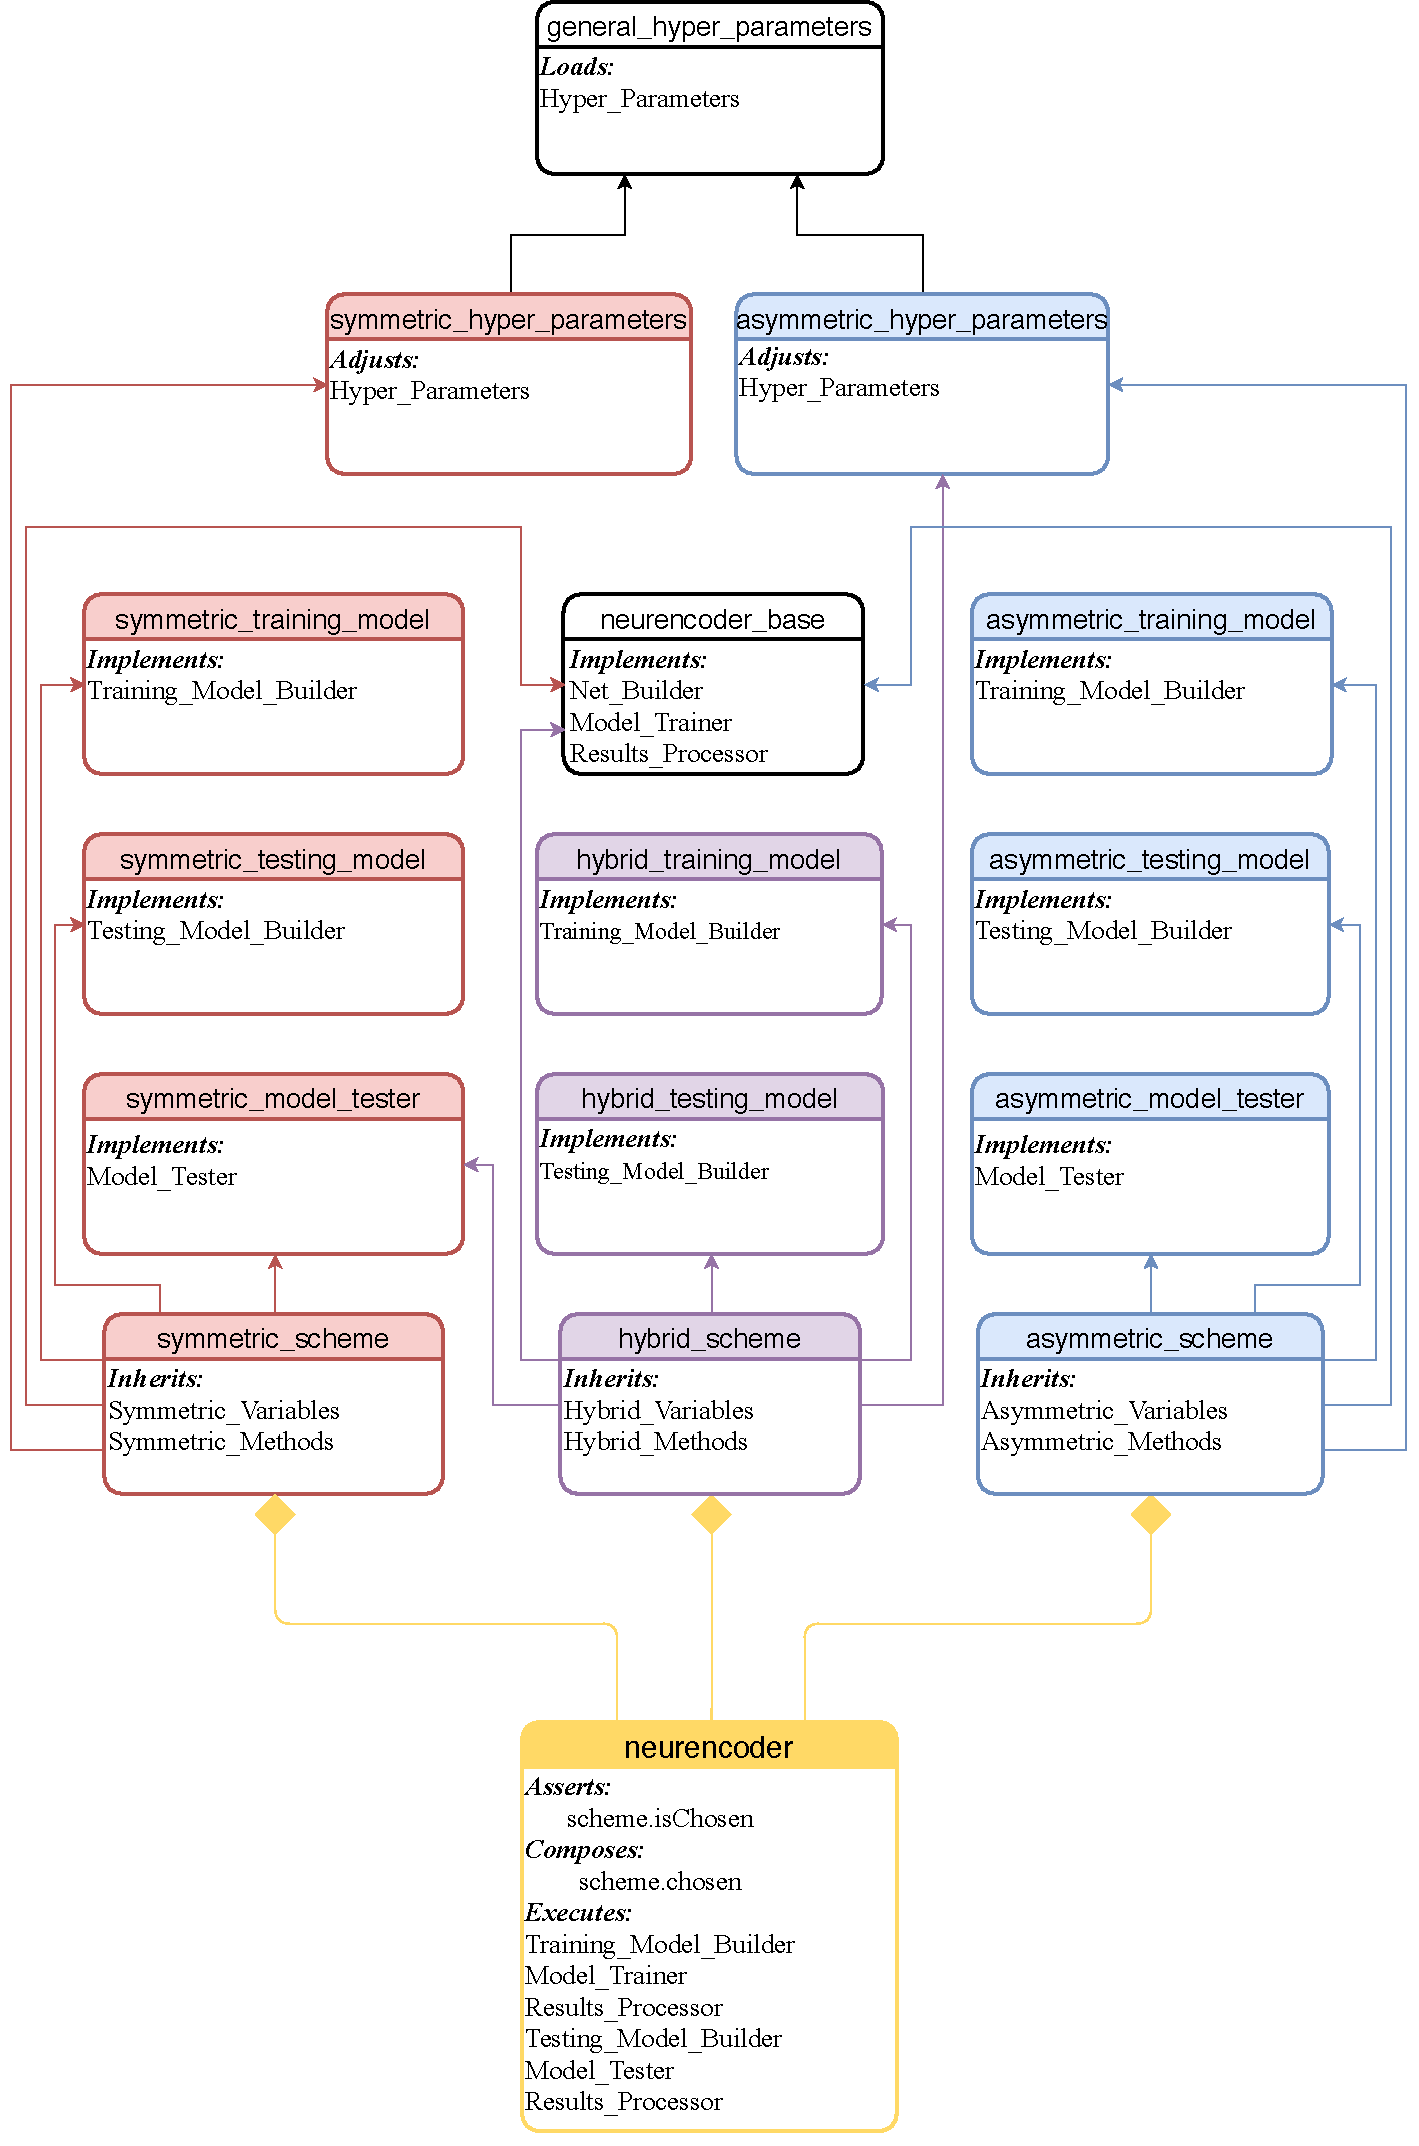
\includegraphics[width = \textwidth]{classDiagram}
	\end{center}
\end{blockfigure}
\newpage
\chapter{Results}\label{sec:results}
\section{\textbf{Thesis Results}}
The results from the various experiments implemented in the project and run daily over the course of 3-4 months can be described as the following:
\begin{itemize}
	\item \textbf{Symmetric Scheme:} experiments conducted were fluctuant in results at few points in time, but can be considered consistent over the entire period, this form of neural cryptography was not the most stable or promising throughout the experiments, but its results are solid and are already on par with results from previous works.
	\item \textbf{Asymmetric Scheme:} experiments conducted were very consistent, and produced very promising results.
	\item \textbf{Hybrid Scheme:} experiments conducted were very consistent, and produced very promising results, in fact the results were very close to those from the Asymmetric Scheme, therefor they need to be studied further to determine why.
\end{itemize}
To ensure the soundness of the experiments, class initiation calls were logged, as well as the method resolution order upon scheme composition.
\subsection{\textbf{Physical Infrastructure \& Consumption}}
\begin{colortable}{Underlying Hardware Infrastructure}
	\textbf{Type} & Graphics Card \\\hline
	\textbf{Manufacturer} & Nvidia \\\hline
	\textbf{Number} & GeForce 920M \\\hline
	\textbf{Compute Power} & 3.5 \\\hline
	\textbf{Clock Rate} & 954 Mhz \\\hline
	\textbf{Cores} & 384 \\\hline
	\textbf{Memory} & 2048 MB
\end{colortable}
\begin{colortable}{Underlying Software Infrastructure}
	\textbf{Type} & \textbf{Name} & \textbf{Version} \\\hline
	OS & Ubuntu & 16.04 \\\hline
	Programming Language   & Python & 3.5 \\\hline
	Parallel Computing Platform & CUDA & 9.0 \\\hline
	Deep Neural Network library & cuDNN & 7.0.5 \\\hline
	ML Framework & Tensorflow GPU & 1.8 \\\hline
	Drivers & Nvidia & 390.30
\end{colortable}
\begin{colortable}{Physical Consumption of Thesis Experiments}
	\textbf{Scheme} & \textbf{Training Steps} & \textbf{Time Consumption} & \textbf{Computational Consumption} & \textbf{Memory Consumption} \\\hline
	Symmetric  & 20,000 & 9-11 Minutes & 80\% & 80\% \\\hline
	Asymmetric  & 20,000 & 11-16 Minutes & 80\% & 80\% \\\hline
	Hybrid  & 20,000 & 11-16 Minutes & 80\% & 80\% \\\hline
\end{colortable}
\newpage
\begin{blockfigure}{Thesis Results - Symmetric Training}
	\begin{center}
		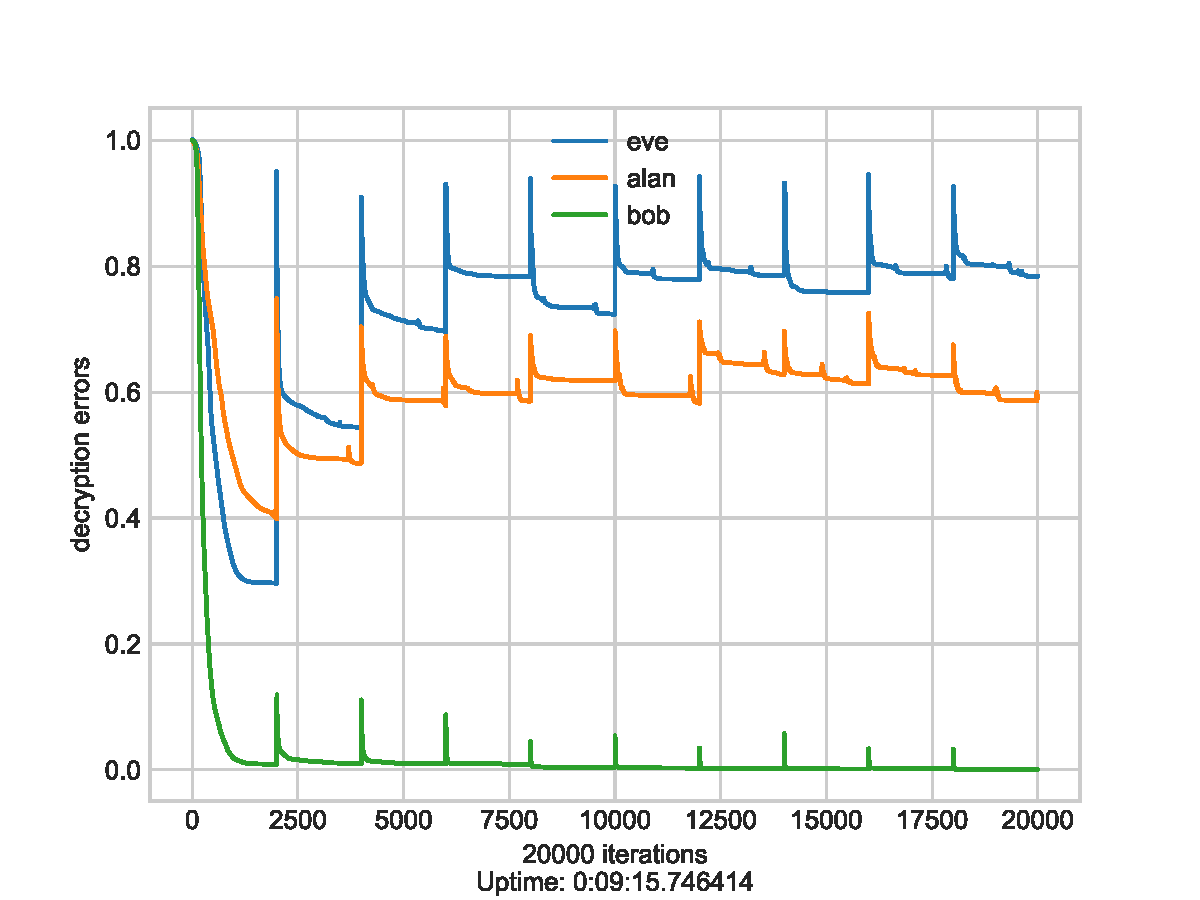
\includegraphics[width = 0.95\textwidth]{neurencoder-symmetric-training}
	\end{center}
\end{blockfigure}
\begin{blockfigure}{Thesis Results - Symmetric Testing}
	\begin{center}
		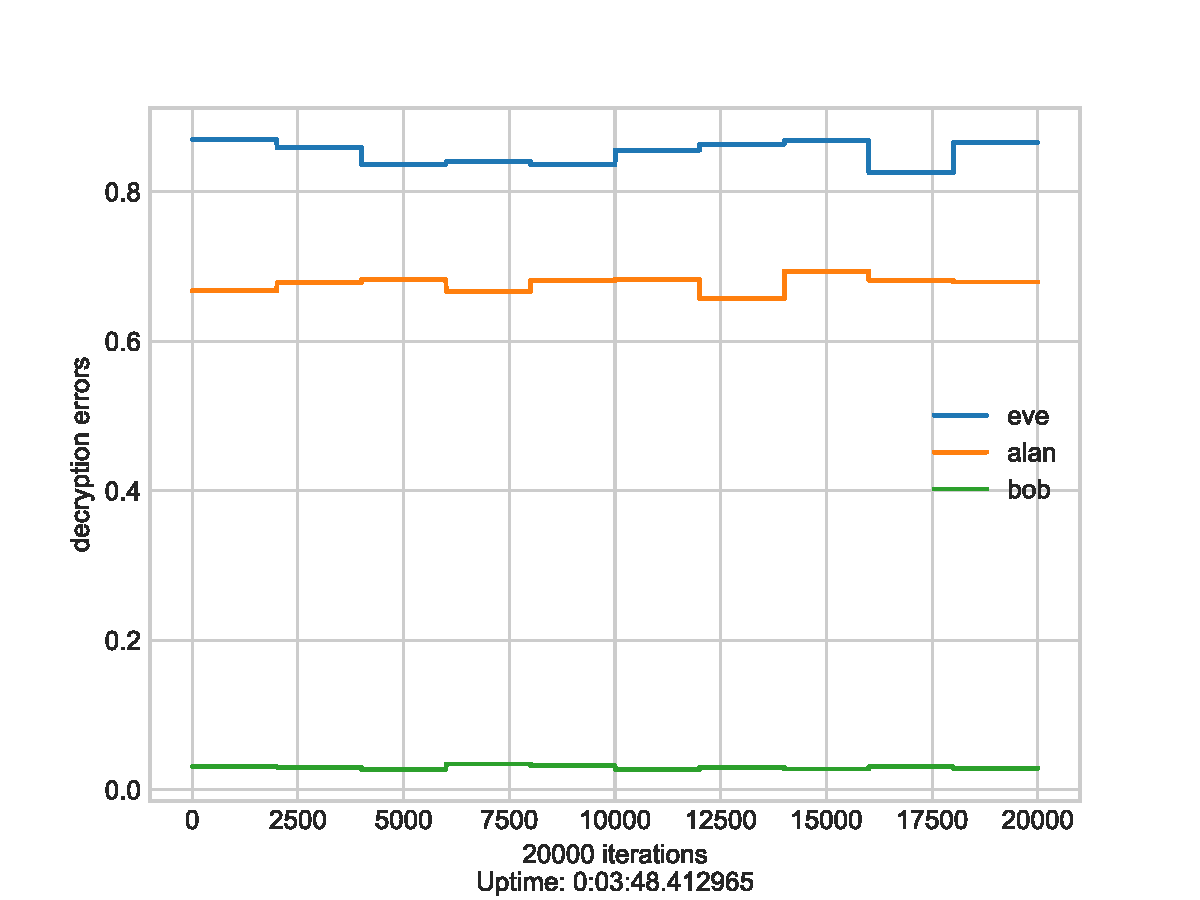
\includegraphics[width = 0.95\textwidth]{neurencoder-symmetric-testing}
	\end{center}
\end{blockfigure}
\newpage
\begin{blockfigure}{Thesis Results - Asymmetric Training}
	\begin{center}
		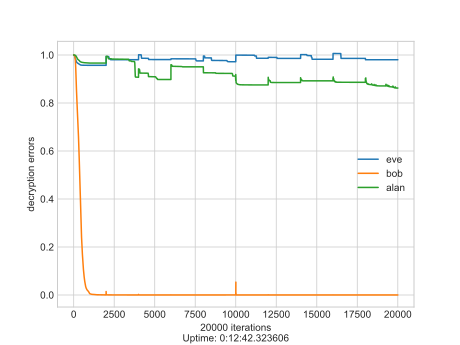
\includegraphics[width = 0.95\textwidth]{neurencoder-asymmetric-training}
	\end{center}
\end{blockfigure}
\begin{blockfigure}{Thesis Results - Asymmetric Testing}
	\begin{center}
		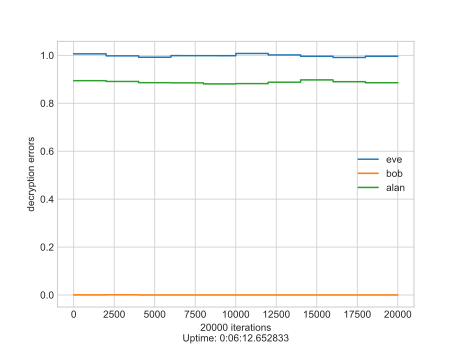
\includegraphics[width = 0.95\textwidth]{neurencoder-asymmetric-testing}
	\end{center}
\end{blockfigure}
\newpage
\begin{blockfigure}{Thesis Results - Hybrid Training}
	\begin{center}
		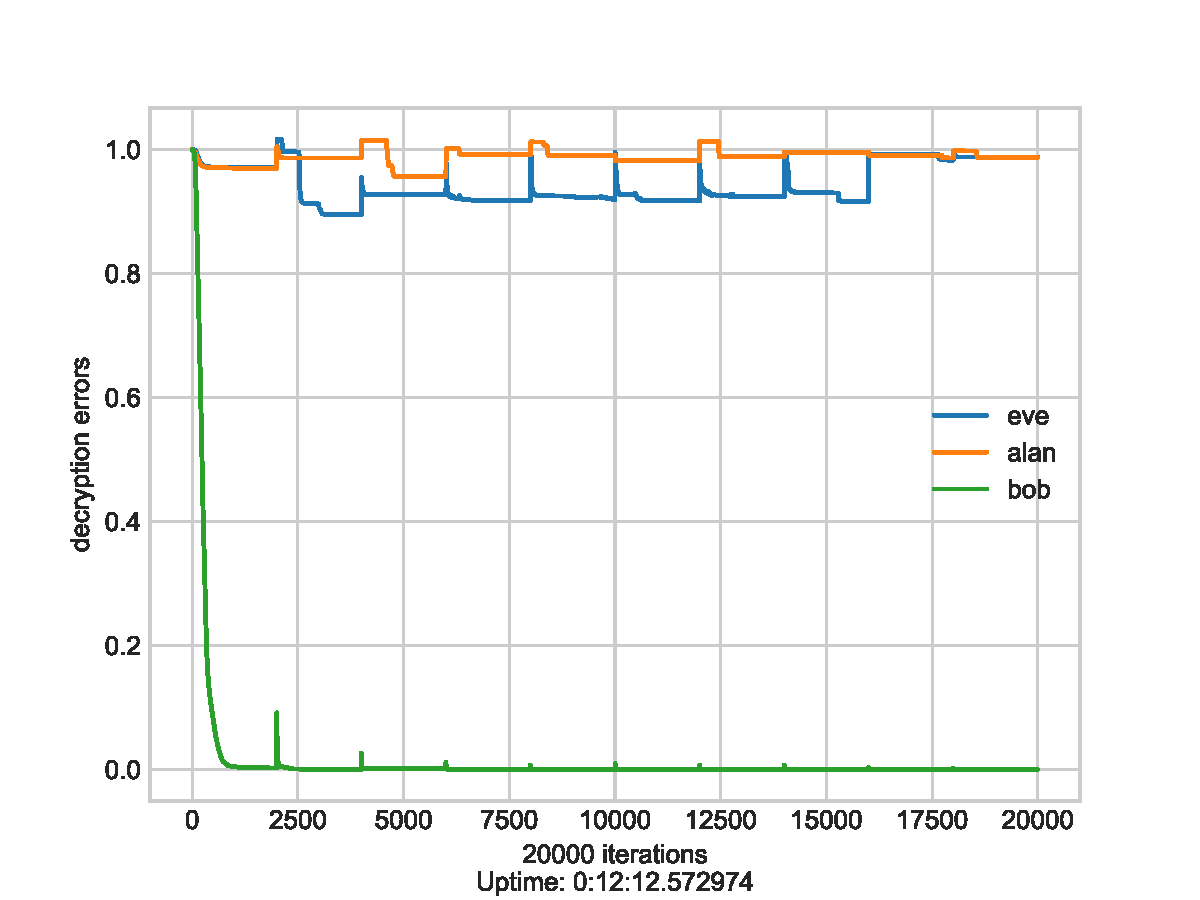
\includegraphics[width = 0.95\textwidth]{neurencoder-hybrid-training}
	\end{center}
\end{blockfigure}
\begin{blockfigure}{Thesis Results - Hybrid Testing}
	\begin{center}
		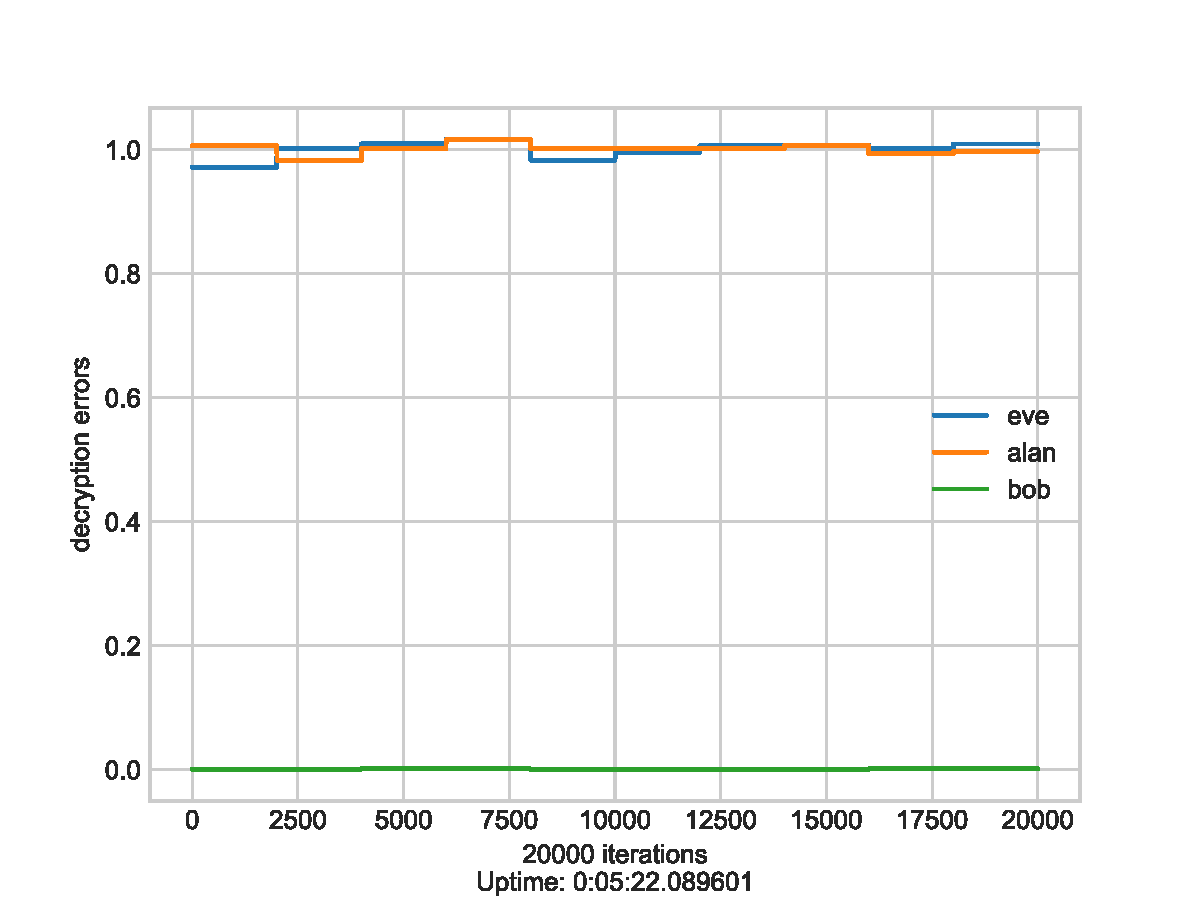
\includegraphics[width = 0.95\textwidth]{neurencoder-hybrid-testing}
	\end{center}
\end{blockfigure}
\newpage
\section{\textbf{Results from Previous Works}}
\subsection{\textbf{Results from Liam Schoneveld}~\citep{nlml/adversarial-neural-cryptography}}
Liam did his experiment on symmetric neural cryptography, with his own Theano implementation of \textit{Learning to Protect Communications with Adversarial Neural Cryptography} ~\citep{DBLP:journals/corr/AbadiA16}, his nets trained for 60 epochs, 2000 iterations each.
But for the sake of comparison with my results, I cloned his code and ran it for 10 epochs (2000 iterations each) on my device, and it produced the following result.
\begin{blockfigure}{Liam Schoneveld - Symmetric Training}
	\begin{center}
		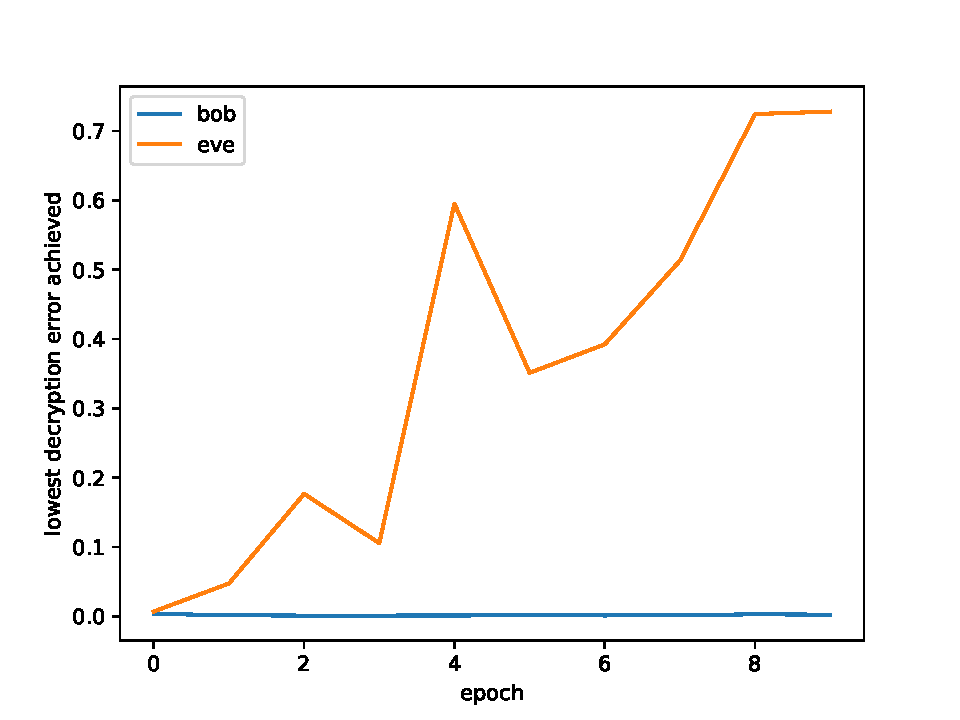
\includegraphics[width = 0.63\textwidth]{nlml_results_conv}
	\end{center}
\end{blockfigure}
\subsection{\textbf{Results from Ankesh Anand}~\citep{ankeshanand/neural-cryptography-tensorflow}}
Ankesh designed his experiment for symmetric neural cryptography, with his own Tensorflow implementation of \textit{Learning to Protect Communications with Adversarial Neural Cryptography} ~\citep{DBLP:journals/corr/AbadiA16}, his system was designed to run for 60 epochs, 2000 iterations each.
But since he does not have result figures readily available, and for the sake of comparison with my results, I cloned his code and ran it for 10 epochs (2000 iterations each) on my device, and it produced the following result.
\begin{blockfigure}{Ankesh Anand - Symmetric Training}
	\begin{center}
		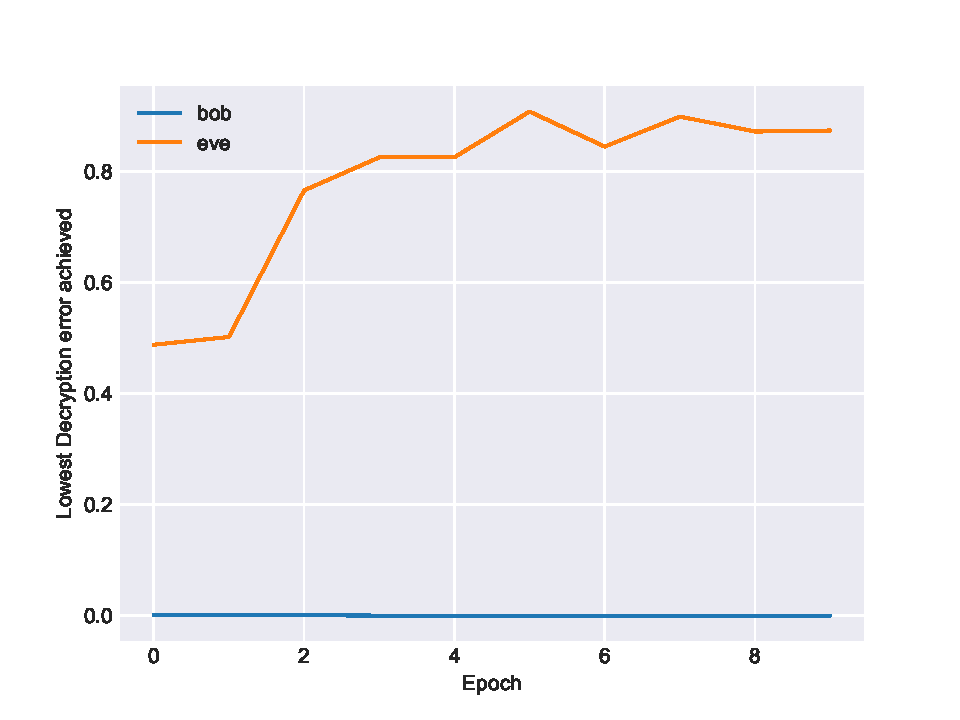
\includegraphics[width = 0.62\textwidth]{ankesh_results_conv}
	\end{center}
\end{blockfigure}
\newpage
\subsection{\textbf{Results from Google Brain} ~\citep{DBLP:journals/corr/AbadiA16}}
The experiments conducted by the authors of the paper \textit{Learning to Protect Communications with Adversarial Neural Cryptography} ~\citep{DBLP:journals/corr/AbadiA16}, were done on both symmetric and asymmetric neural cryptography, they used a larger batch size of 4096, and ran their experiments for longer periods.\\
For symmetric neural cryptography, they used the same scheme presented in this thesis.
\begin{blockfigure}{Google Brain - Symmetric Training}
	\begin{center}
		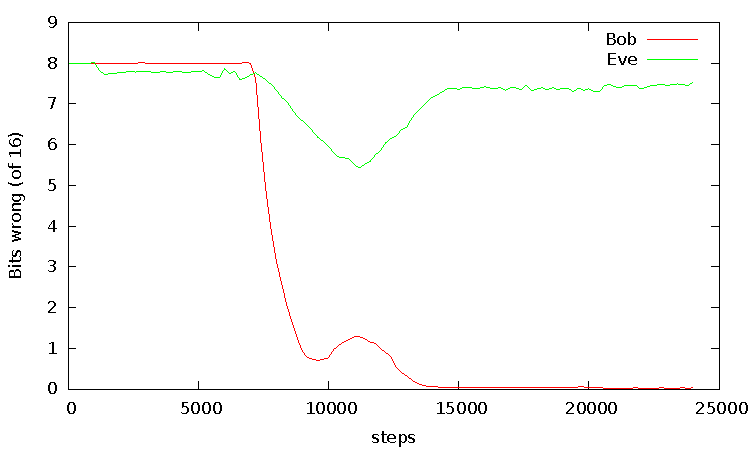
\includegraphics[width = 0.65\textwidth]{cryptolearn_batch_tighter}
	\end{center}
\end{blockfigure}\\
As for asymmetric neural cryptography, they used a slightly different scheme, mainly omitting the private key generator.
\begin{blockfigure}{Google Brain - Asymmetric Scheme}
	\begin{center}
		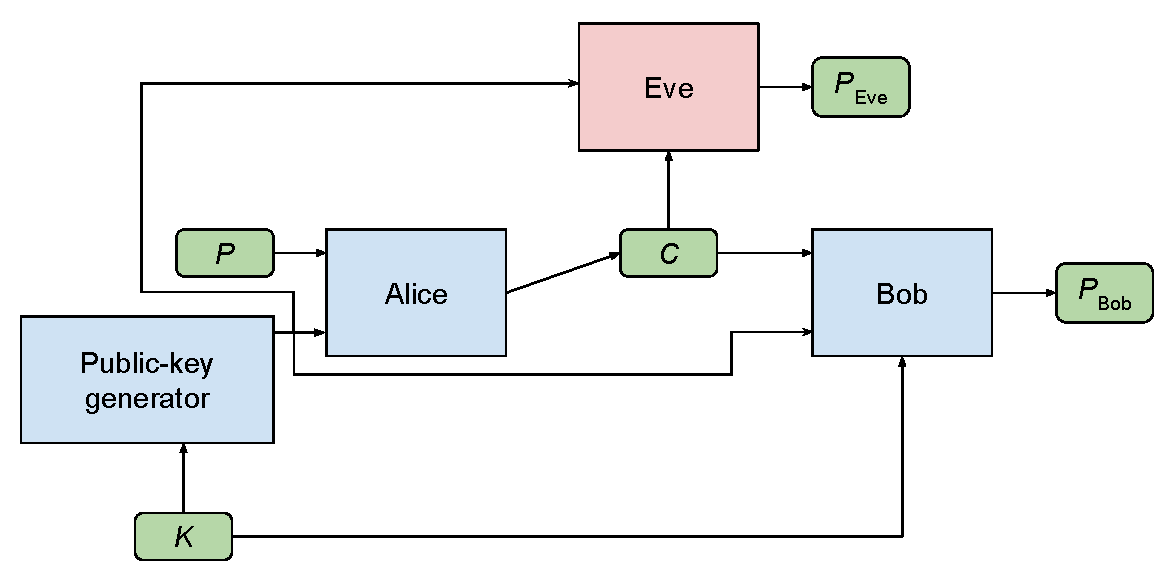
\includegraphics[width = 0.65\textwidth]{asymm}
	\end{center}
\end{blockfigure}
\begin{blockfigure}{Google Brain - Asymmetric Training}
	\begin{center}
		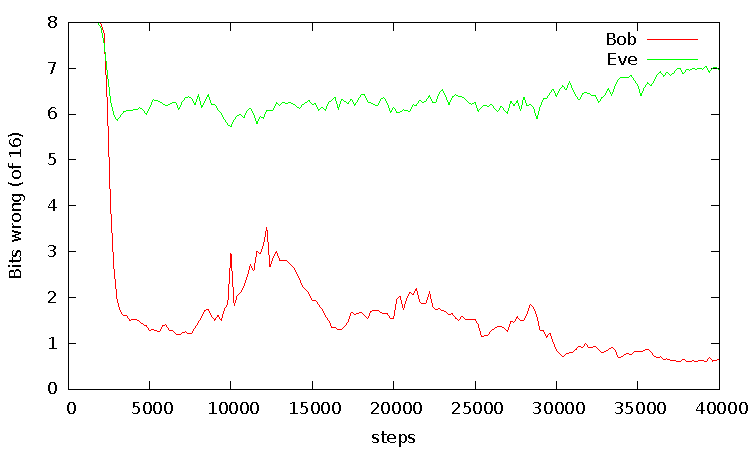
\includegraphics[width = 0.65\textwidth]{pubkey_bob_v_eve}
	\end{center}
\end{blockfigure}
\newpage
\chapter{Conclusion}\label{sec:conclusion}
\begin{center}
	\begin{minipage}{0.8\textwidth}
		\justify
		This dissertation provided an example showcasing that neural nets can learn to minimize loss in integrity of information while maximizing confidentiality. It has also provided an example of how to transfer what they have learned to be applied in different cryptographic settings.
	\end{minipage}
\end{center}
\section*{\textbf{Points of Future Research}}
\begin{itemize}[nosep]
	\item The contrast between how neural nets rely on floating point distributions opposite to the randomized binary of the plain text they try to reproduce, which warrants an exploration of whether such contrast is relevant to the positive results (and therefor giving a false positive), or the opposite.
	\item The statistical properties of the bottlenecks between the different nets beyond the least squared means, as more study into these statistical properties is needed (e.g. KL-Divergence), similar to the research seen in the paper "Context-Aware Generative Adversarial Privacy
	"~\citep{e19120656}.
	\item Modern modes of cryptographic operations, which is considered an important corner stone in modern cryptography, further research into teaching neural nets how to synthesize rigorous modes of operation need to be done, as a starting point, we can consider the CTR Mode of block-ciphers.~\citep{BlockCipherModes}
	\item A production ready solution to neural cryptography, as more real-world designs need to be implemented for these systems to be tested on real life data.
\end{itemize}
\section*{\textbf{Proposed General Considerations}}
	\begin{itemize}
		\item \textbf{Constructing a production ready crypto-system:} by reducing each plain message sample size to one character, while keeping the key sample size large to preserve confidentiality and maintain convolution ability.
		\item \textbf{Countering cryptanalysis in the new system:} by considering the entire batch as a block, and infusing each plain message batch with a key batch containing the same key in each sample, which should preserve relation locality in data.
		\item \textbf{Testing for the effects of floating point distributions:} by infusing the decoder's output layer with a Bernouli Distribution~\citep{http://mathworld.wolfram.com/BernoulliDistribution.html} layer, to force the decoder to optimize for binary output, this will force the encoder in turn to provide better ciphers to account for the limited binary range of the decoder's output.
	\end{itemize}
\section*{\textbf{Proposed Model-Structure Considerations}}
\begin{itemize}
	\item An RNN infused 1D Convolution.\footnote{RNN: recurrent neural network\citep{Hochreiter1997}}
	\item A VAE infused scheme.\footnote{VAE: variational auto encoder\citep{2013arXiv1312.6114K}}
	\item A scheme with neuroevolution as its optimization process.\footnote{Neuroevolution is the process of using a genetic algorithm to evolve (optimize) a neural network.~\citep{Floreano2008}~\citep{DBLP:journals/corr/abs-1803-00657}\citep{GeneticLander}}
\end{itemize}
\newpage
\begin{blockfigure}{RNN Infused 1D Convolution}
	\begin{center}
		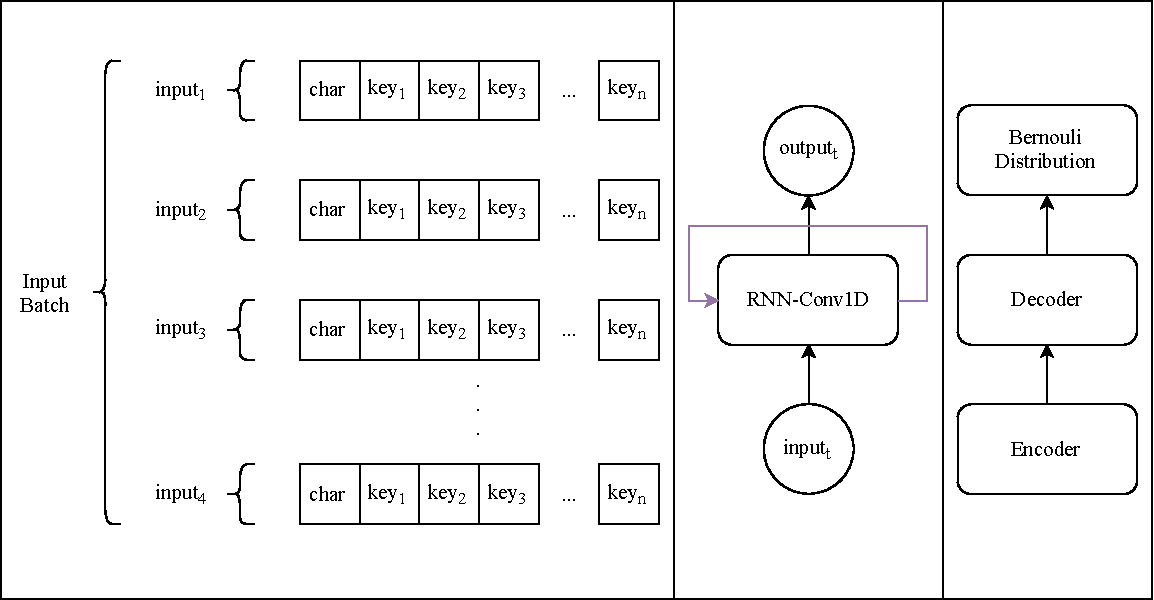
\includegraphics[width = 0.9\textwidth]{suggestion_rnn_conv1d}
	\end{center}
\end{blockfigure}
\begin{blockfigure}{VAE Infused Scheme}
	\begin{center}
		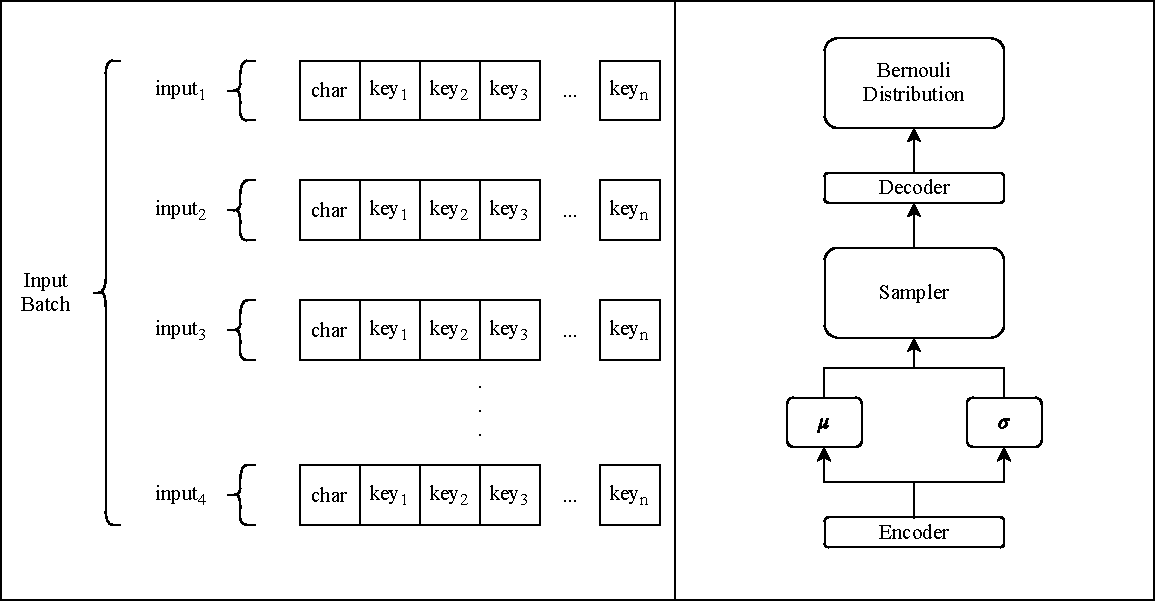
\includegraphics[width = 0.9\textwidth]{suggestion_vae}
	\end{center}
\end{blockfigure}
\begin{blockfigure}{Neuroevolution of Neural Cryptography}
	\begin{center}
		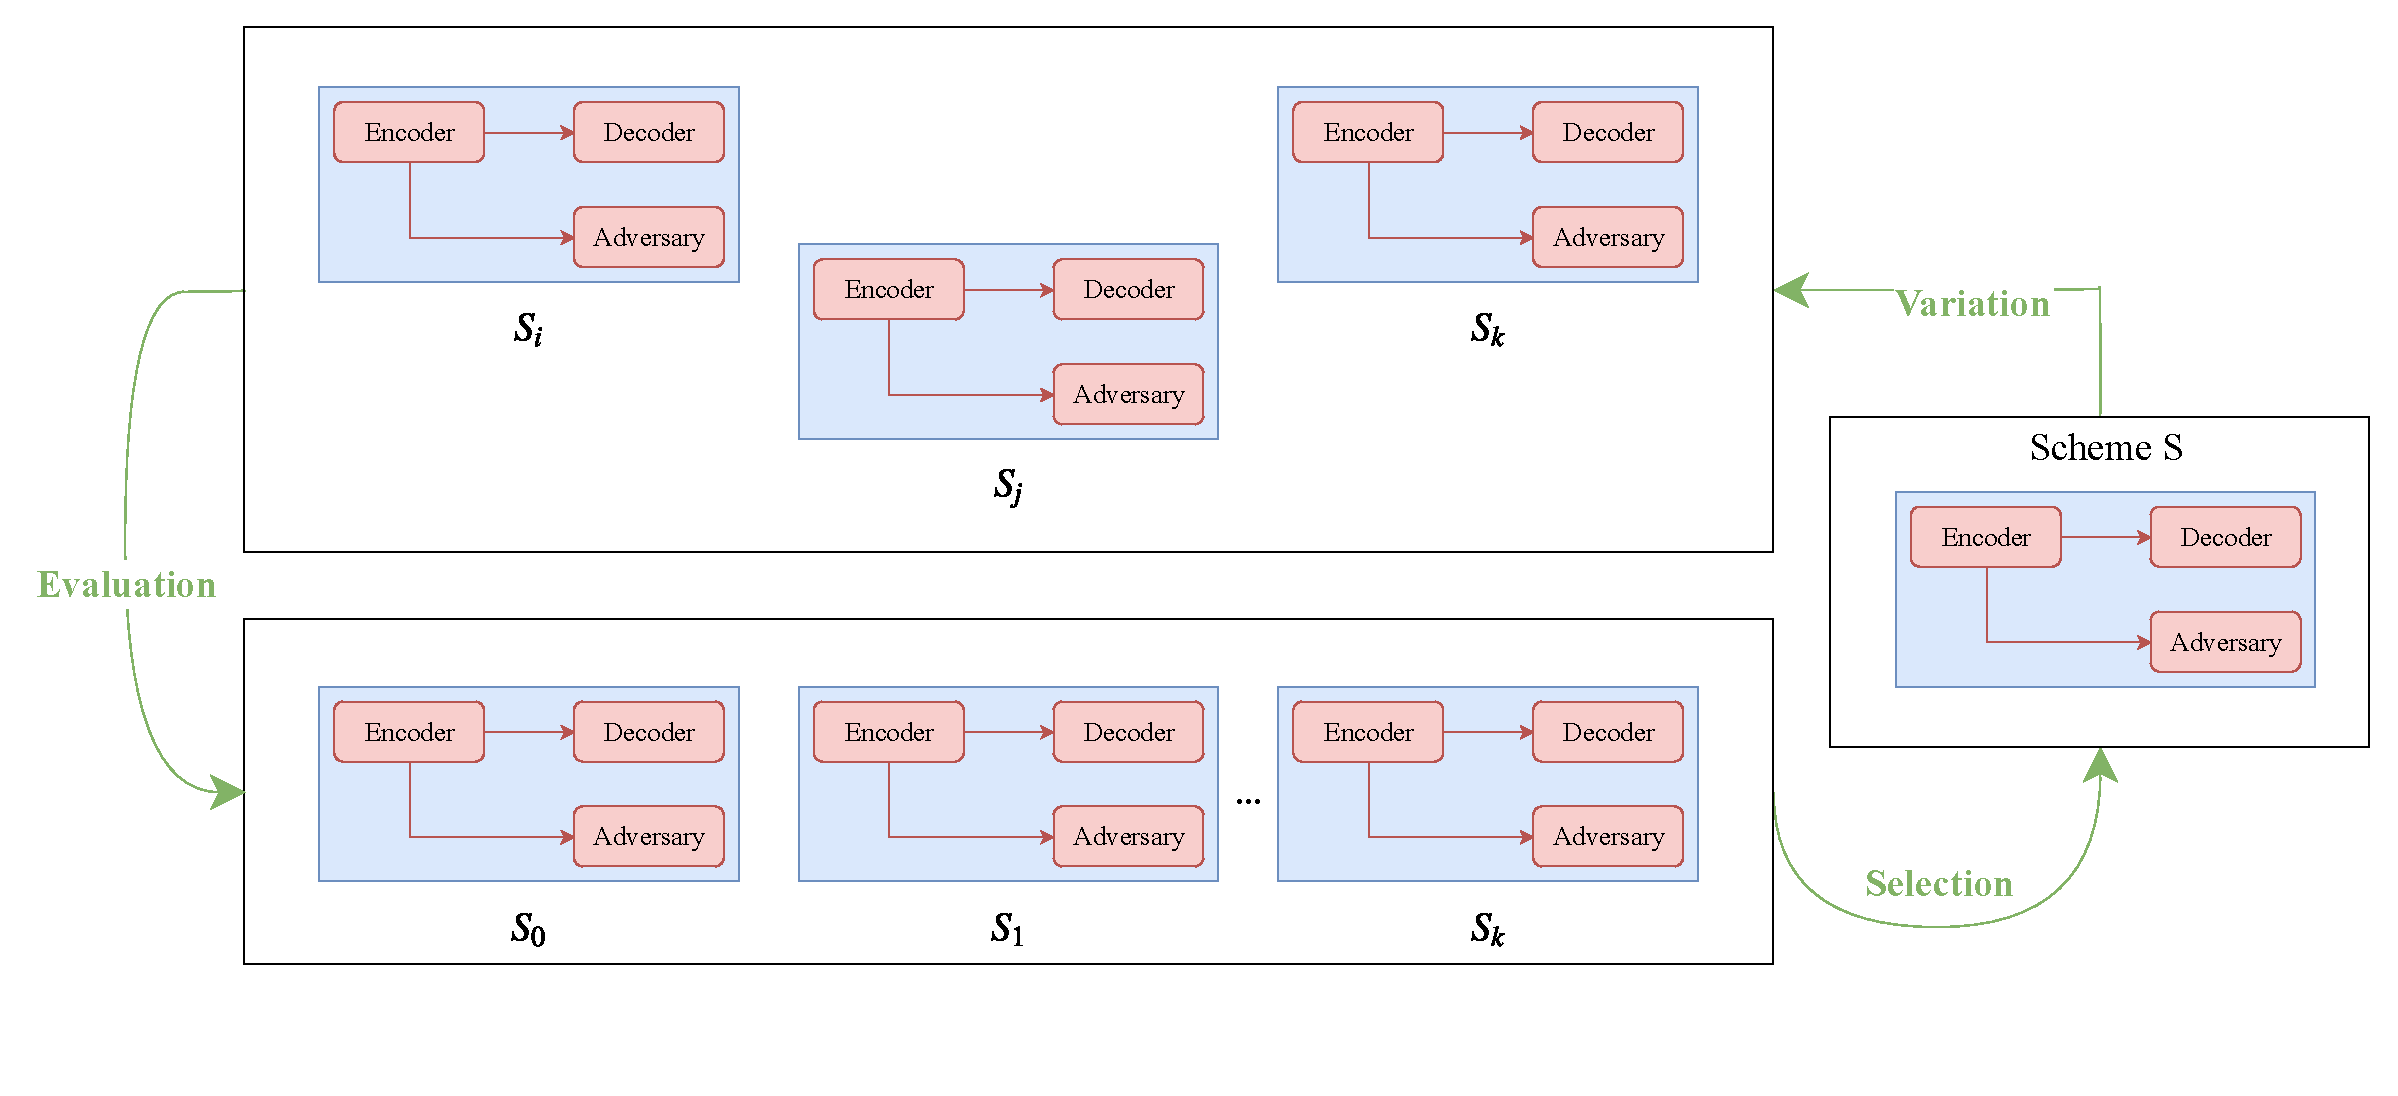
\includegraphics[width = 0.8\textwidth]{GAC}
	\end{center}
\end{blockfigure}
\newpage
\chapter*{Appendix}
\section*{\textbf{Spatial Relations in Cryptography and Cryptanalysis}}\label{appendix:1}
As we try to make neural nets learn cryptography that can parallel modern cryptographic algorithms, we need to teach neural nets to understand patterns in data which resemble patterns found in cryptography and cryptanalysis.\\
These patterns, as I see them, can be titled like the following:
\begin{itemize}
	\item Cryptographic Patterns.
	\item Cryptanalytic Patterns.
\end{itemize}
\subsection*{\textbf{Cryptographic Patterns}}
\blockquote{Assume the existence of a matching operator $ \rhd $ for matching a value
$ v $ against a pattern $ p $, written $ v \rhd p $. Such a construct should be used upon input or decryption in a process calculus, and the general idea is then that a process $ v \rhd p $ in $ P $ first verifies that $ v $ matches $ p $; if this is the case the continuation process is updated with any newly mapped variables, and executed, otherwise the execution will be blocked.
The matching $ T(n, m) \rhd T(y, m) \lhd [y] $ in $ P $ should succeed because the tuple $ T(n, m) $ matches $ T(y, m) $. This results in the mapping of the variable $ y $ to the name $ n $ in the continuation process $ P $. The matching $ T(n, m) \rhd T(y, y) \lhd [y] $ in $ P $ on the other hand would not succeed as both n and m cannot match the pattern y, and thus further execution is garbled.~\citep{Nielsen2007CryptographicPM}}
The cryptographic patterns described here are mathematically constructed with a mapping function using an operator $ \rhd $, and from this abstract construction of cryptography we can deduce the necessity for a great level of mapping of local spacial locations from plaintext to ciphertext.
\subsection*{\textbf{Cryptanalytic Patterns}}
Cryptanalysis relies heavily on statistical analysis to find patterns in ciphertext to use them later on in breaking the encryption, and therefor when building a crypto-system it's essential to build it with statistical hypothesis testing in mind.\citep{7031850}\\
Crypto Statistical Analysis of the ciphertext can be run on both global spatial locations and local spacial locations, but by taking a lesson from frequency analysis, it is safe to assume the priority of running the analysis on global spatial locations first in order to deduce where the local spatial locations occur, and thus the emphasis in cryptanalysis is on finding global spatial relations in ciphertext.\\
\begin{hypothesis}\end{hypothesis}
	\begin{itemize}[nosep]
		\item Cryptographic Patterns are constructed by mapping local spatial relations from the plaintext to the ciphertext.
		\item Cryptanalysis Patterns are global spatial relations in ciphertext that facilitate finding and analyzing local spatial relations from ciphertext to plaintext. 
	\end{itemize}
\newpage
\chapter*{Acknowledgments}
I would like to thank the following entities for their help and support:
\begin{itemize}
	\item \textbf{Prof. Giovanni De Gasperis}, Associate Professor at UnivAQ: for his guidance, patience and supervision of this thesis.
	\item \textbf{The International Office at UnivAQ}: for their financial support which made completing this thesis possible.
	\item \textbf{Ankesh Anand}, PhD student in the machine learning laboratory at the University of Montreal: for his correspondence to my emails regarding questions about his previous work in this area\citep{ankeshanand/neural-cryptography-tensorflow}.
	\item \textbf{Justin Johnson}, PhD student in the Stanford Vision Lab: for his correspondence to my emails regarding his work on the lecture notes of the course titled \textit{"CS231n Convolutional Neural Networks for Visual Recognition"}\citep{cs231n}.
	\item \textbf{Prof. Dr.-Ing. Christof Paar}, Chair for Embedded Security at Ruhr Universitat Bochum: for his correspondence to my emails regarding my inquiries about abstract differences between cryptography and cryptanalysis, and his insight about the importance of cryptographic modes of operation.
\end{itemize}
\newpage
\medskip
\bibliographystyle{unsrt}
\bibliography{neurencoder}
\end{document}